% Options for packages loaded elsewhere
\PassOptionsToPackage{unicode}{hyperref}
\PassOptionsToPackage{hyphens}{url}
%
\documentclass[
]{memoir}
\usepackage{amsmath,amssymb}
\usepackage{lmodern}
\usepackage{iftex}
\ifPDFTeX
  \usepackage[T1]{fontenc}
  \usepackage[utf8]{inputenc}
  \usepackage{textcomp} % provide euro and other symbols
\else % if luatex or xetex
  \usepackage{unicode-math}
  \defaultfontfeatures{Scale=MatchLowercase}
  \defaultfontfeatures[\rmfamily]{Ligatures=TeX,Scale=1}
  \setmainfont[]{Roboto}
  \setsansfont[]{Clancy}
  \setmonofont[Scale=0.9]{Roboto Mono}
\fi
% Use upquote if available, for straight quotes in verbatim environments
\IfFileExists{upquote.sty}{\usepackage{upquote}}{}
\IfFileExists{microtype.sty}{% use microtype if available
  \usepackage[]{microtype}
  \UseMicrotypeSet[protrusion]{basicmath} % disable protrusion for tt fonts
}{}
\makeatletter
\@ifundefined{KOMAClassName}{% if non-KOMA class
  \IfFileExists{parskip.sty}{%
    \usepackage{parskip}
  }{% else
    \setlength{\parindent}{0pt}
    \setlength{\parskip}{6pt plus 2pt minus 1pt}}
}{% if KOMA class
  \KOMAoptions{parskip=half}}
\makeatother
\usepackage{xcolor}
\IfFileExists{xurl.sty}{\usepackage{xurl}}{} % add URL line breaks if available
\IfFileExists{bookmark.sty}{\usepackage{bookmark}}{\usepackage{hyperref}}
\hypersetup{
  pdftitle={PHCM9795 Foundations of Biostatistics},
  pdfauthor={Pilot Notes for R},
  hidelinks,
  pdfcreator={LaTeX via pandoc}}
\urlstyle{same} % disable monospaced font for URLs
\usepackage{color}
\usepackage{fancyvrb}
\newcommand{\VerbBar}{|}
\newcommand{\VERB}{\Verb[commandchars=\\\{\}]}
\DefineVerbatimEnvironment{Highlighting}{Verbatim}{commandchars=\\\{\}}
% Add ',fontsize=\small' for more characters per line
\usepackage{framed}
\definecolor{shadecolor}{RGB}{248,248,248}
\newenvironment{Shaded}{\begin{snugshade}}{\end{snugshade}}
\newcommand{\AlertTok}[1]{\textcolor[rgb]{0.94,0.16,0.16}{#1}}
\newcommand{\AnnotationTok}[1]{\textcolor[rgb]{0.56,0.35,0.01}{\textbf{\textit{#1}}}}
\newcommand{\AttributeTok}[1]{\textcolor[rgb]{0.77,0.63,0.00}{#1}}
\newcommand{\BaseNTok}[1]{\textcolor[rgb]{0.00,0.00,0.81}{#1}}
\newcommand{\BuiltInTok}[1]{#1}
\newcommand{\CharTok}[1]{\textcolor[rgb]{0.31,0.60,0.02}{#1}}
\newcommand{\CommentTok}[1]{\textcolor[rgb]{0.56,0.35,0.01}{\textit{#1}}}
\newcommand{\CommentVarTok}[1]{\textcolor[rgb]{0.56,0.35,0.01}{\textbf{\textit{#1}}}}
\newcommand{\ConstantTok}[1]{\textcolor[rgb]{0.00,0.00,0.00}{#1}}
\newcommand{\ControlFlowTok}[1]{\textcolor[rgb]{0.13,0.29,0.53}{\textbf{#1}}}
\newcommand{\DataTypeTok}[1]{\textcolor[rgb]{0.13,0.29,0.53}{#1}}
\newcommand{\DecValTok}[1]{\textcolor[rgb]{0.00,0.00,0.81}{#1}}
\newcommand{\DocumentationTok}[1]{\textcolor[rgb]{0.56,0.35,0.01}{\textbf{\textit{#1}}}}
\newcommand{\ErrorTok}[1]{\textcolor[rgb]{0.64,0.00,0.00}{\textbf{#1}}}
\newcommand{\ExtensionTok}[1]{#1}
\newcommand{\FloatTok}[1]{\textcolor[rgb]{0.00,0.00,0.81}{#1}}
\newcommand{\FunctionTok}[1]{\textcolor[rgb]{0.00,0.00,0.00}{#1}}
\newcommand{\ImportTok}[1]{#1}
\newcommand{\InformationTok}[1]{\textcolor[rgb]{0.56,0.35,0.01}{\textbf{\textit{#1}}}}
\newcommand{\KeywordTok}[1]{\textcolor[rgb]{0.13,0.29,0.53}{\textbf{#1}}}
\newcommand{\NormalTok}[1]{#1}
\newcommand{\OperatorTok}[1]{\textcolor[rgb]{0.81,0.36,0.00}{\textbf{#1}}}
\newcommand{\OtherTok}[1]{\textcolor[rgb]{0.56,0.35,0.01}{#1}}
\newcommand{\PreprocessorTok}[1]{\textcolor[rgb]{0.56,0.35,0.01}{\textit{#1}}}
\newcommand{\RegionMarkerTok}[1]{#1}
\newcommand{\SpecialCharTok}[1]{\textcolor[rgb]{0.00,0.00,0.00}{#1}}
\newcommand{\SpecialStringTok}[1]{\textcolor[rgb]{0.31,0.60,0.02}{#1}}
\newcommand{\StringTok}[1]{\textcolor[rgb]{0.31,0.60,0.02}{#1}}
\newcommand{\VariableTok}[1]{\textcolor[rgb]{0.00,0.00,0.00}{#1}}
\newcommand{\VerbatimStringTok}[1]{\textcolor[rgb]{0.31,0.60,0.02}{#1}}
\newcommand{\WarningTok}[1]{\textcolor[rgb]{0.56,0.35,0.01}{\textbf{\textit{#1}}}}
\usepackage{longtable,booktabs,array}
\usepackage{calc} % for calculating minipage widths
% Correct order of tables after \paragraph or \subparagraph
\usepackage{etoolbox}
\makeatletter
\patchcmd\longtable{\par}{\if@noskipsec\mbox{}\fi\par}{}{}
\makeatother
% Allow footnotes in longtable head/foot
\IfFileExists{footnotehyper.sty}{\usepackage{footnotehyper}}{\usepackage{footnote}}
\makesavenoteenv{longtable}
\usepackage{graphicx}
\makeatletter
\def\maxwidth{\ifdim\Gin@nat@width>\linewidth\linewidth\else\Gin@nat@width\fi}
\def\maxheight{\ifdim\Gin@nat@height>\textheight\textheight\else\Gin@nat@height\fi}
\makeatother
% Scale images if necessary, so that they will not overflow the page
% margins by default, and it is still possible to overwrite the defaults
% using explicit options in \includegraphics[width, height, ...]{}
\setkeys{Gin}{width=\maxwidth,height=\maxheight,keepaspectratio}
% Set default figure placement to htbp
\makeatletter
\def\fps@figure{htbp}
\makeatother
\setlength{\emergencystretch}{3em} % prevent overfull lines
\providecommand{\tightlist}{%
  \setlength{\itemsep}{0pt}\setlength{\parskip}{0pt}}
\setcounter{secnumdepth}{5}
\usepackage{booktabs}
\usepackage{float}

\floatstyle{boxed}
\newfloat{program}{thp}{lop}
\floatname{program}{Output}

\renewcommand{\chaptername}{Module}
\renewcommand*{\chapnamefont}{\normalfont\HUGE\bfseries\sffamily}
\renewcommand*{\chapnumfont}{\normalfont\HUGE\bfseries\sffamily}
\renewcommand*{\chaptitlefont}{\normalfont\HUGE\bfseries\sffamily}

\setsecheadstyle{\sffamily}% Set \section style
\setsubsecheadstyle{\sffamily}% Set \subsection style
\setsubsubsecheadstyle{\sffamily}% Set \subsubsection style

\setlrmarginsandblock{3.5cm}{2.5cm}{*}
\setulmarginsandblock{2.5cm}{*}{1}
\checkandfixthelayout 

\raggedright
\raggedbottom
\usepackage{array}
\usepackage{caption}
\usepackage{graphicx}
\usepackage{siunitx}
\usepackage[normalem]{ulem}
\usepackage{colortbl}
\usepackage{multirow}
\usepackage{hhline}
\usepackage{calc}
\usepackage{tabularx}
\usepackage{threeparttable}
\usepackage{wrapfig}
\usepackage{adjustbox}
\usepackage{hyperref}
\ifLuaTeX
  \usepackage{selnolig}  % disable illegal ligatures
\fi
\usepackage[]{natbib}
\bibliographystyle{plainnat}

\title{PHCM9795 Foundations of Biostatistics}
\author{Pilot Notes for R}
\date{Term 2, 2022}

\begin{document}
\maketitle

{
\setcounter{tocdepth}{1}
\tableofcontents
}
\hypertarget{introduction}{%
\chapter*{Introduction}\label{introduction}}
\addcontentsline{toc}{chapter}{Introduction}

These notes provide an introduction to R and instructions on how to conduct the analyses introduced in Foundations of Biostatistics.

This is the first year that R has been offered as an option. I am keen to receive feedback about the notes and your experience learning R. Please get in touch if anything is unclear, or you have any questions or suggestions.

\hypertarget{introduction-to-r-and-rstudio}{%
\chapter{Introduction to R and RStudio}\label{introduction-to-r-and-rstudio}}

INCLUDE:

\begin{itemize}
\tightlist
\item
  decide on skim vs summary vs jmv::describe
\item
  case sensitive
\item
  how to get help (online, google, etc)
\item
  functions that use (data=, var=) vs functions that use an object (i.e.~data\$var)
\item
  how to specify a column from a dataframe
\item
  don't give up!
\item
  tidyverse?
\end{itemize}

\hypertarget{learning-outcomes}{%
\section*{Learning outcomes}\label{learning-outcomes}}
\addcontentsline{toc}{section}{Learning outcomes}

By the end of this Module, you will be able to:

\begin{itemize}
\tightlist
\item
  understand the difference between R and RStudio
\item
  navigate the RStudio interface
\item
  input and import data into R
\item
  use R to summarise data
\item
  perform basic data transformations
\item
  assign variable and value labels
\item
  understand the difference between saving R data and saving R output
\item
  copy R output to a standard word processing package
\end{itemize}

\hypertarget{introduction-1}{%
\section{Introduction}\label{introduction-1}}

``R is a language and environment for statistical computing and graphics.'' {[}\url{https://www.r-project.org/about.html}{]}. It is an open-source programming language, used mainly for statistics. It is increasingly used in health research, as well as in other fields such as econometrics and social science. The aim of these notes is to introduce the R language within the RStudio environment, and to introduce the commands and procedures that are directly relevant to this course. There is so much more to R than we can cover in these notes. Relevant information will be provided throughout the course, and we will provide further references that you can explore if you are interested.

\hypertarget{r-vs-rstudio}{%
\section{R vs RStudio}\label{r-vs-rstudio}}

At its heart, R is a programming language. When you install R on your computer, you are installing the language and its resources, as well as a very basic interface for using R. You can write and run R code using R, but we don't recommend it.

RStudio is an ``Integrated Development Environment'' that runs R while also providing useful tools to help you as you're writing code and analysing data. Think of R as the engine which does the work, and RStudio as the wrapper which provides a more user-friendly way to interact with R.

\hypertarget{installing-r-and-rsudio}{%
\section{Installing R and RSudio}\label{installing-r-and-rsudio}}


\includegraphics[width=0.8\linewidth]{img/Rlogo} \includegraphics[width=0.8\linewidth]{img/RStudio-logo-flat}

To install R on your computer:

\begin{enumerate}
\def\labelenumi{\arabic{enumi}.}
\tightlist
\item
  Download the R installer:

  \begin{enumerate}
  \def\labelenumii{\alph{enumii}.}
  \tightlist
  \item
    for Windows:
  \item
    for MacOS:
  \end{enumerate}
\item
  Install R by running the installer and following the installation instructions. The default settings are fine.
  \textbf{Note for macOS:} if you are running macOS 10.8 or later, you will need to install an additional application called XQuartz, which is available at \url{https://www.xquartz.org/}. Download the latest installer (XQuartz-2.8.1.dmg as of April 2022), and install it in the usual way.
\item
  Open the R program. You should see a screen as below:
\end{enumerate}

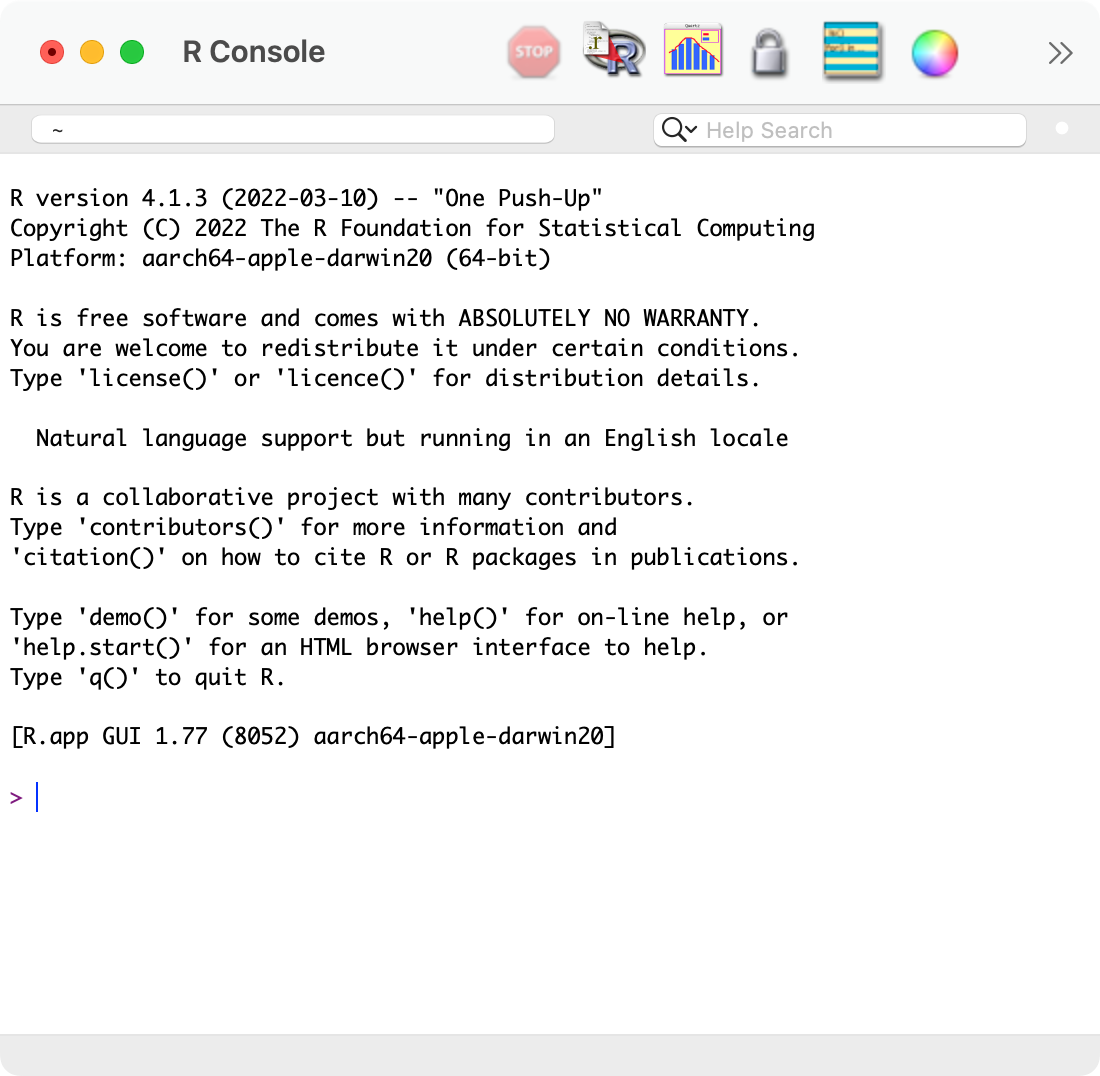
\includegraphics[width=0.8\linewidth]{img/R-screenshot}

Near the bottom of the R screen, you will find the ``\textgreater{}'' symbol which represents the command line. If you type \texttt{1\ +\ 2} into the command line and then hit enter you should get:

\texttt{{[}1{]}\ 3}

This is R performing your calculation, with the \texttt{{[}1{]}} indicating that the solution to \texttt{1\ +\ 2} is a vector of size 1. We will talk about vectors later.

At this point, close R - we will not interact with R like this in the future. {[}HOW TO CLOSE R{]}

To install RStudio on your computer:

\begin{enumerate}
\def\labelenumi{\arabic{enumi}.}
\tightlist
\item
  Make sure you have already installed R, and verified that it is working.
\item
  Download the RStudio desktop installer at: \url{https://www.rstudio.com/products/rstudio/download}. Ensure that you select the RStudio Desktop (Free) installer in the first column.
\item
  Install RStudio by running the installer and following the installation instructions. The default settings are fine.
\item
  Open RStudio, which will appear as below:
\end{enumerate}

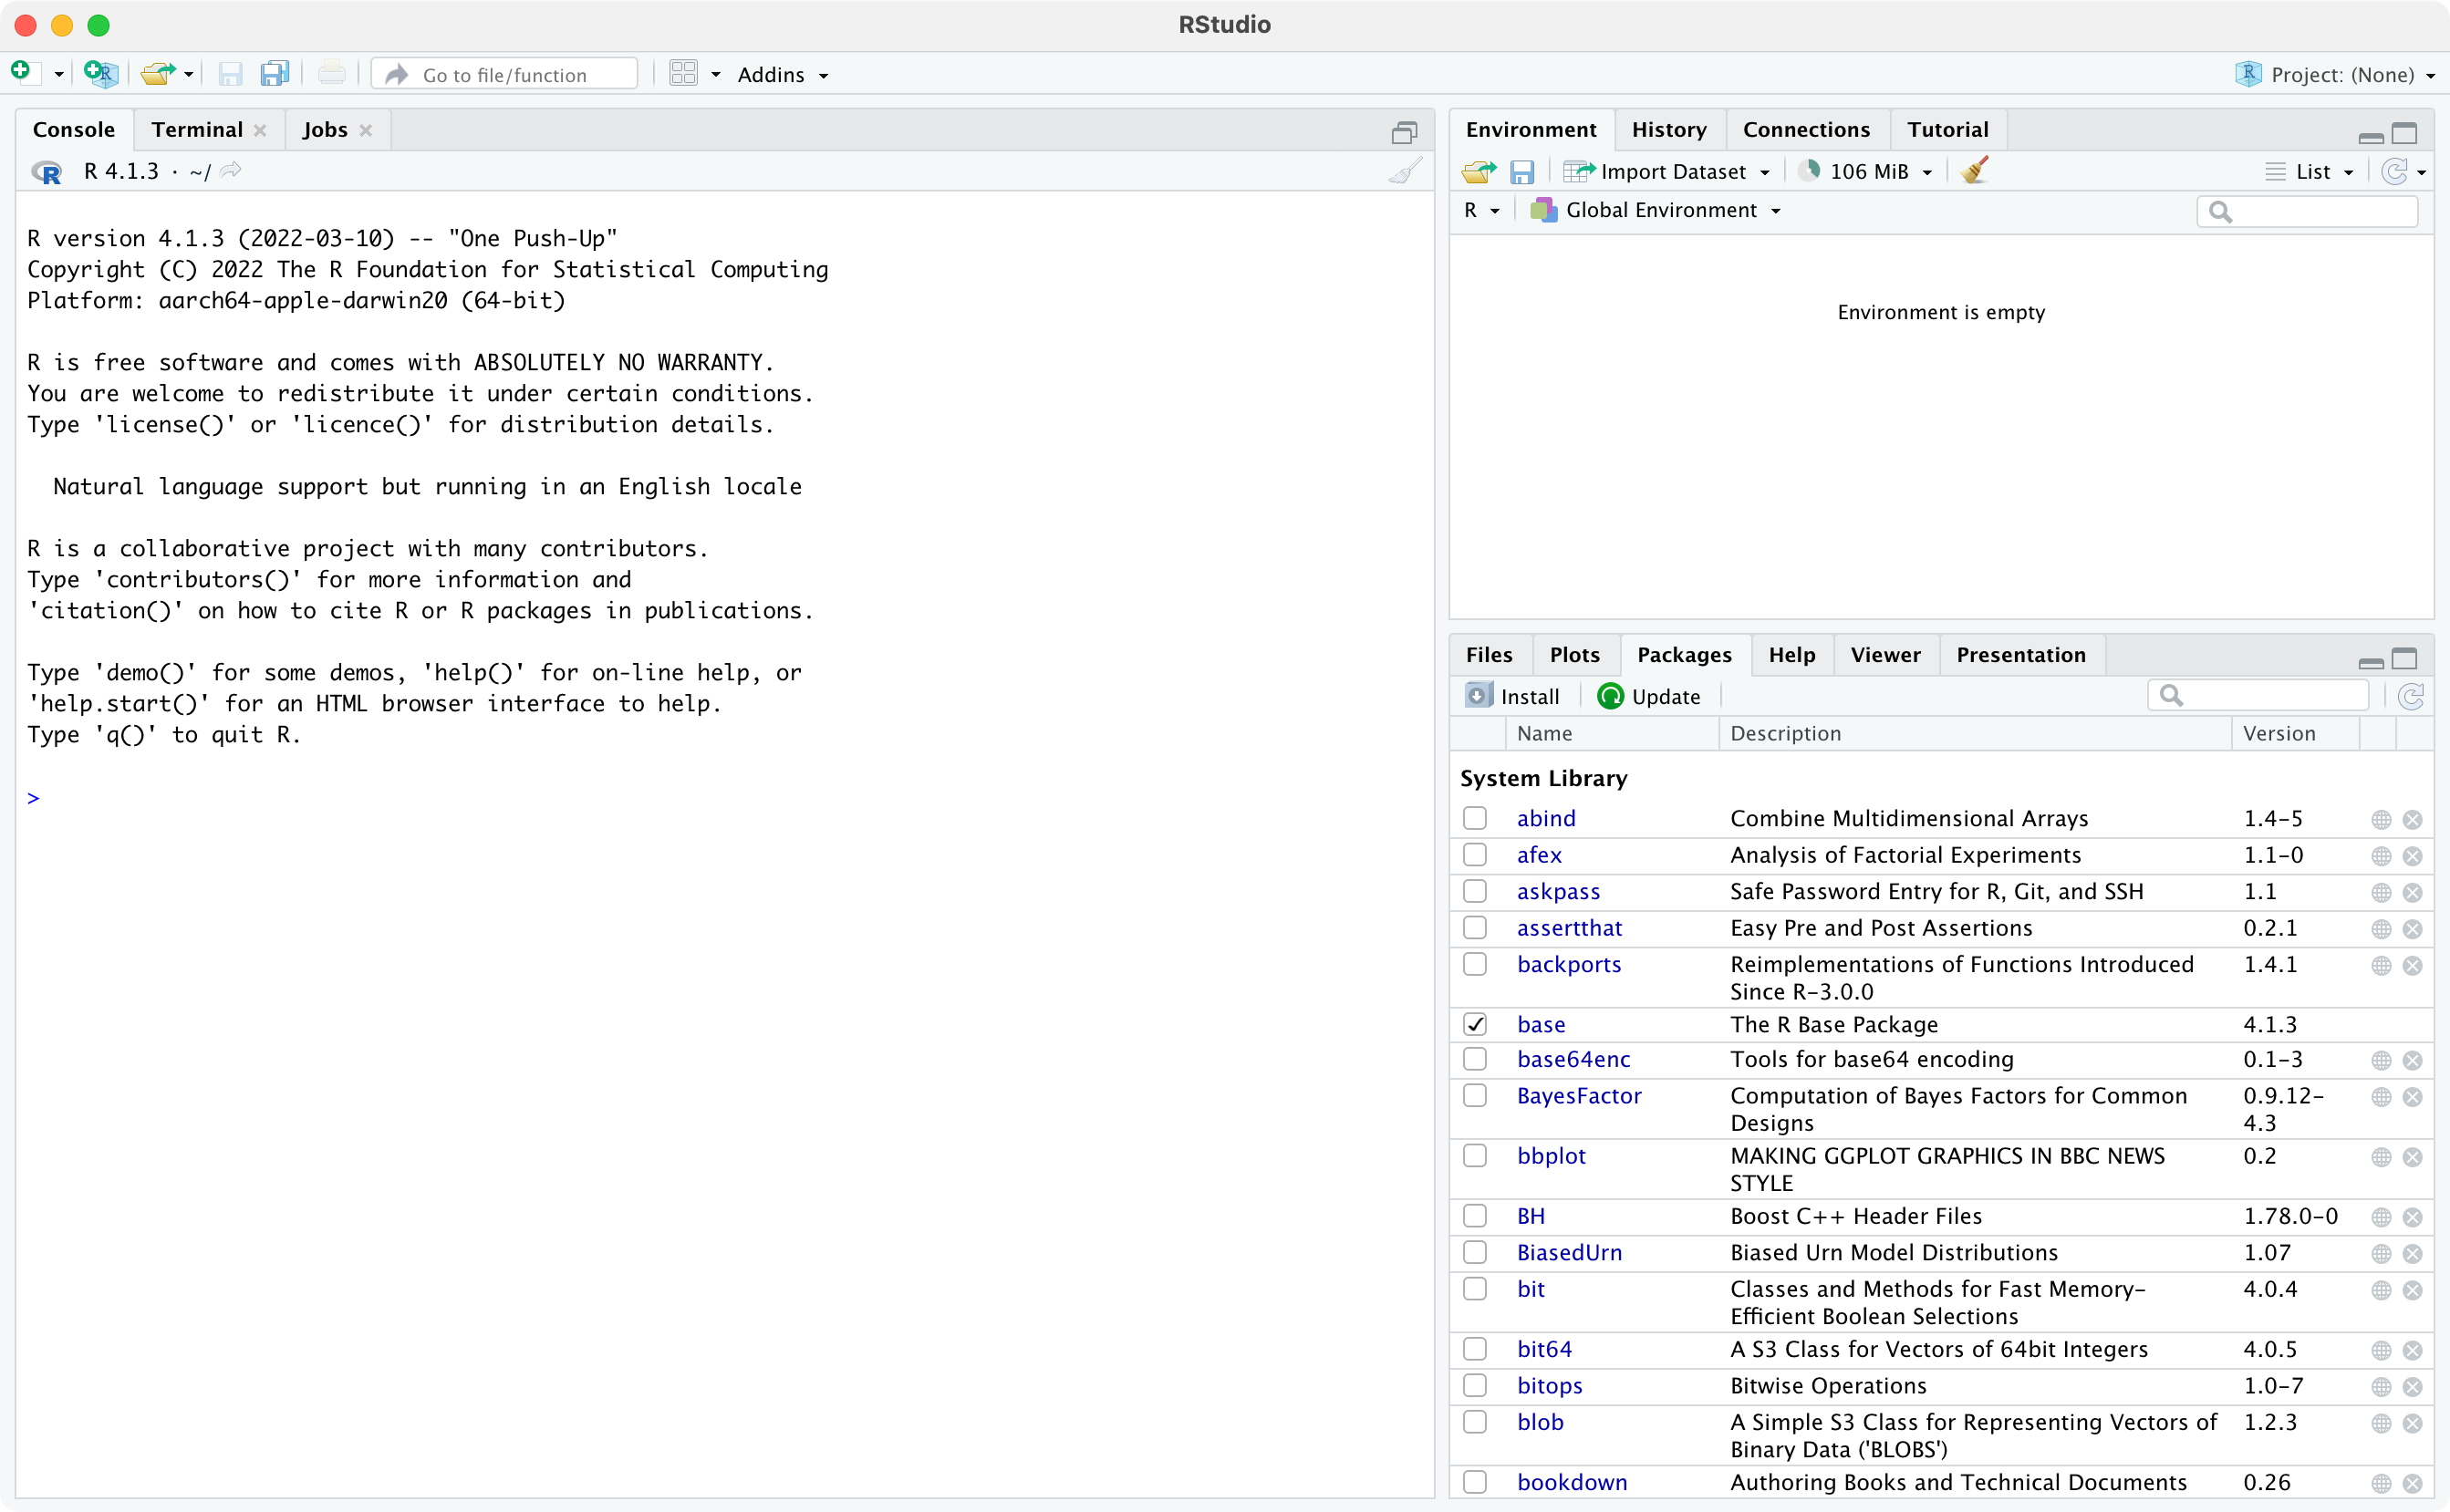
\includegraphics[width=1\linewidth]{img/RStudio-screenshot-01}

Locate the command line symbol ``\textgreater{}'' at the bottom of the left-hand panel. Type \texttt{1\ +\ 2} into the command line and hit enter, and you will see:

\texttt{{[}1{]}\ 3}

This confirms that RStudio is running correctly, and calling the R language to correctly calculate the sum between 1 and 2!

RStudio currently comprises three window panes, and we will discuss these later.

\hypertarget{simpleR}{%
\section{A simple R analysis}\label{simpleR}}

In this very brief section, we will introduce R by calculating the average of six ages.

To begin, open a new R Script by choosing \textbf{File \textgreater{} New file \textgreater{} R Script }. A script (or a program) is a collection of commands that are sequentially processed by R. You can also type Ctrl+Shift+N in Windows, or Command+Shift+N in MacOS to open a new script in RStudio, or click the \textbf{New File} button at the top of the RStudio window.

You should now see four window panes, as below. In the top-left window, type the following (replacing my name with yours, and including today's date):

\begin{Shaded}
\begin{Highlighting}[]
\CommentTok{\# Author: Timothy Dobbins}
\CommentTok{\# Date: 5 April 2022}
\CommentTok{\# Purpose: My first R script}

\NormalTok{age }\OtherTok{\textless{}{-}} \FunctionTok{c}\NormalTok{(}\DecValTok{20}\NormalTok{, }\DecValTok{25}\NormalTok{, }\DecValTok{23}\NormalTok{, }\DecValTok{29}\NormalTok{, }\DecValTok{21}\NormalTok{, }\DecValTok{27}\NormalTok{)}
\FunctionTok{summary}\NormalTok{(age)}
\end{Highlighting}
\end{Shaded}

Your screen should look something like:

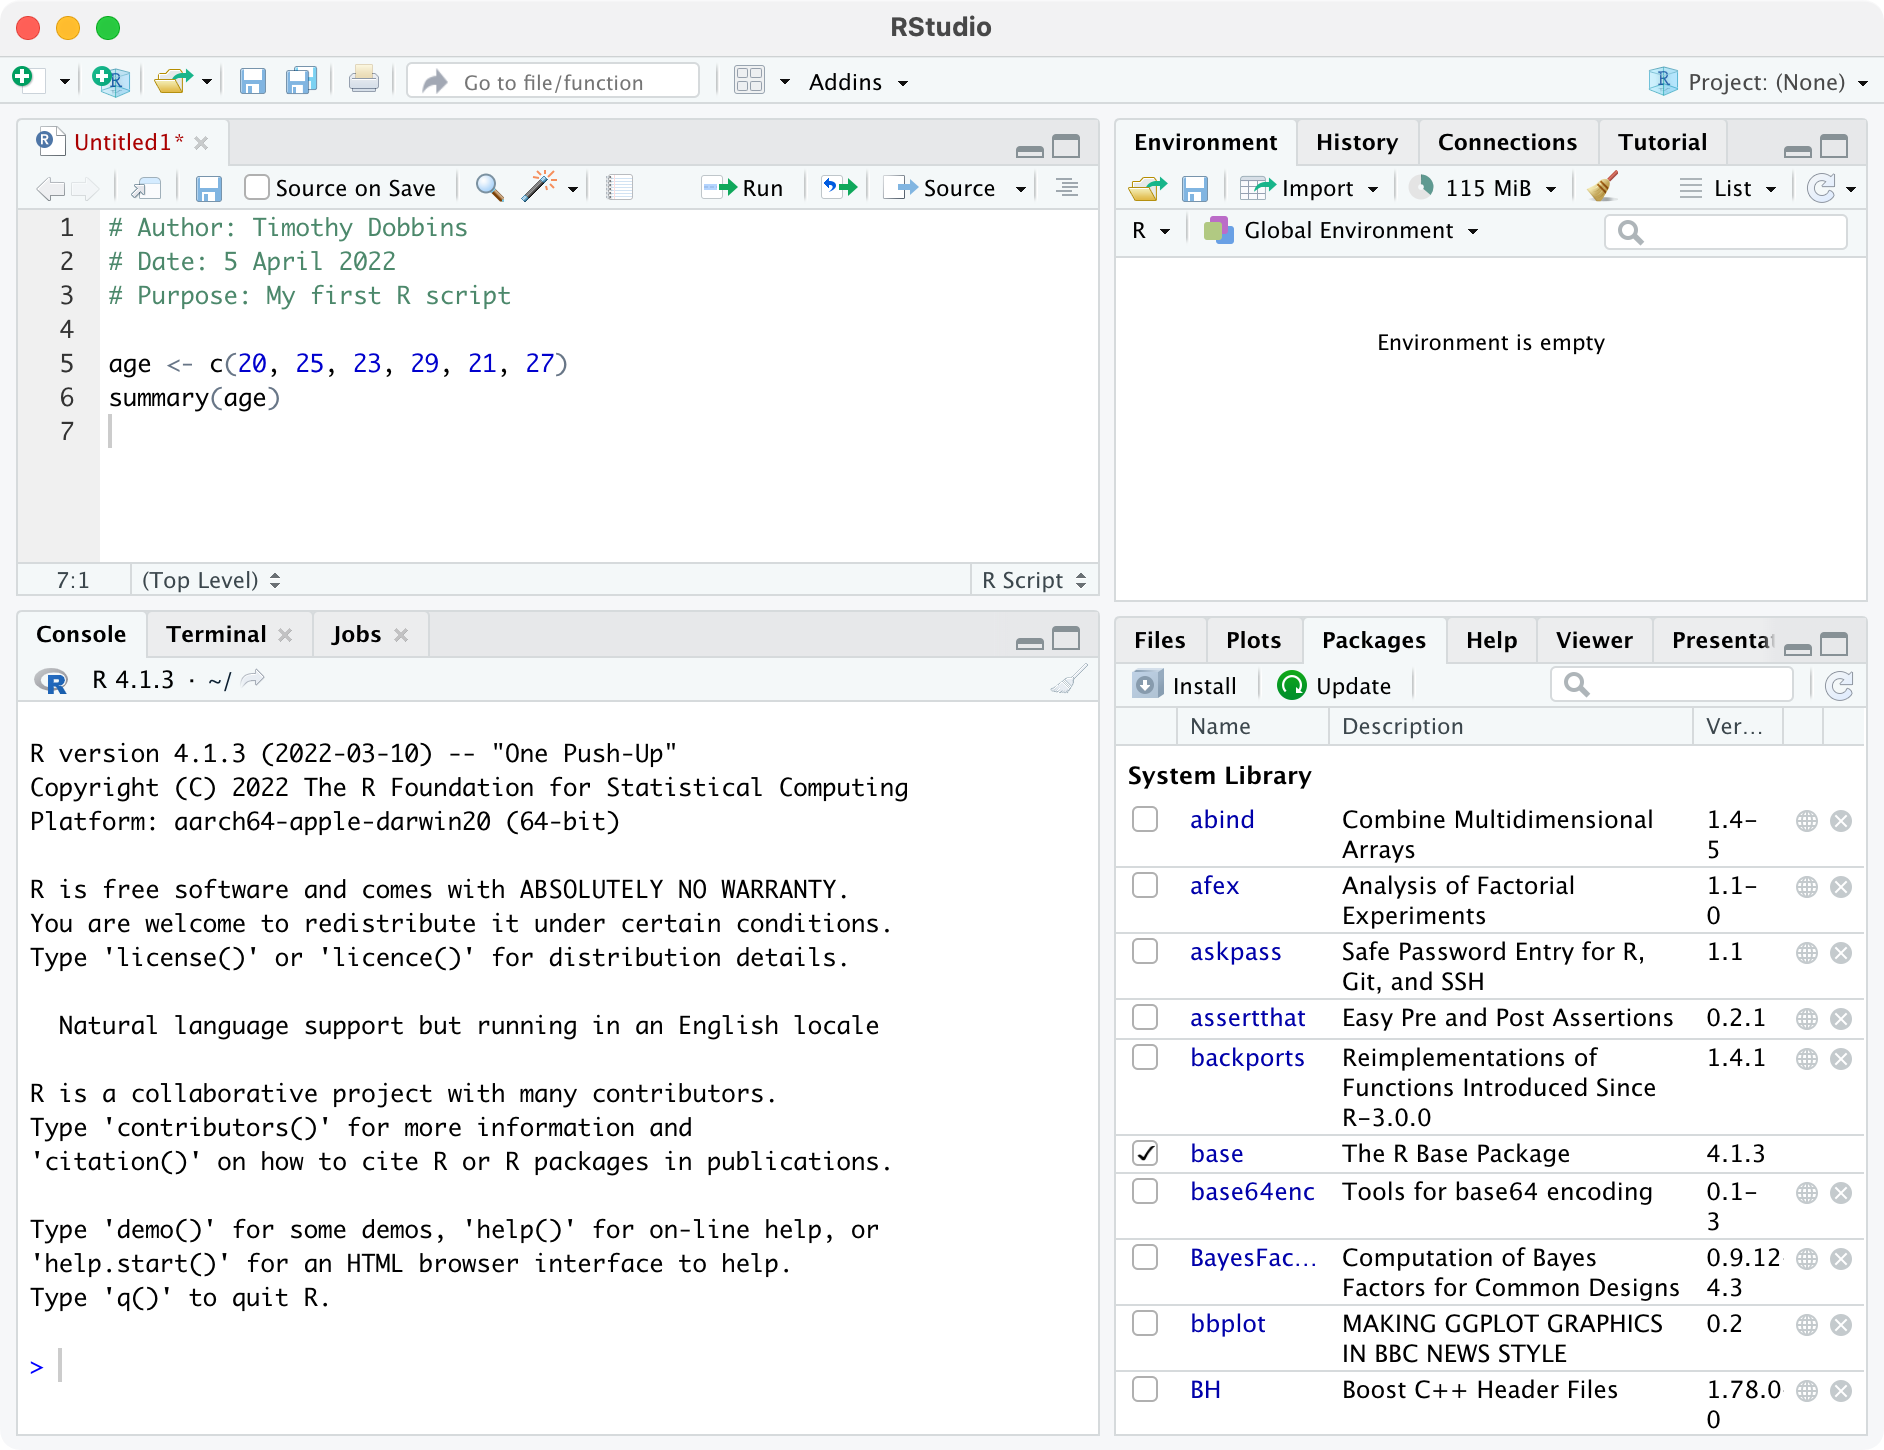
\includegraphics[width=1\linewidth]{img/RStudio-screenshot-02}

To run your script, choose \textbf{Code \textgreater{} Run Region \textgreater{} Run All}. You will see your code appear in the bottom-right window, with the following output:

\begin{Shaded}
\begin{Highlighting}[]
\SpecialCharTok{\textgreater{}} \CommentTok{\# Author: Timothy Dobbins}
\ErrorTok{\textgreater{}} \CommentTok{\# Date: 5 April 2022}
\ErrorTok{\textgreater{}} \CommentTok{\# Purpose: My first R script}
\ErrorTok{\textgreater{}} 
\ErrorTok{\textgreater{}}\NormalTok{ age }\OtherTok{\textless{}{-}} \FunctionTok{c}\NormalTok{(}\DecValTok{20}\NormalTok{, }\DecValTok{25}\NormalTok{, }\DecValTok{23}\NormalTok{, }\DecValTok{29}\NormalTok{, }\DecValTok{21}\NormalTok{, }\DecValTok{27}\NormalTok{)}

\SpecialCharTok{\textgreater{}} \FunctionTok{summary}\NormalTok{(age)}
\NormalTok{   Min. 1st Qu.  Median    Mean 3rd Qu.    Max. }
  \FloatTok{20.00}   \FloatTok{21.50}   \FloatTok{24.00}   \FloatTok{24.17}   \FloatTok{26.50}   \FloatTok{29.00} 
\end{Highlighting}
\end{Shaded}

We will explain the key parts of this script later, but for now, you have entered six ages and calculated the mean age (along with five other summary statistics).

\hypertarget{the-rstudio-environment}{%
\section{The RStudio environment}\label{the-rstudio-environment}}

Now that we have seen a simple example of how to use R within RStudio, let's describe the RStudio environment. Let's assume that you have opened a new script editor, and you have four windows as below:

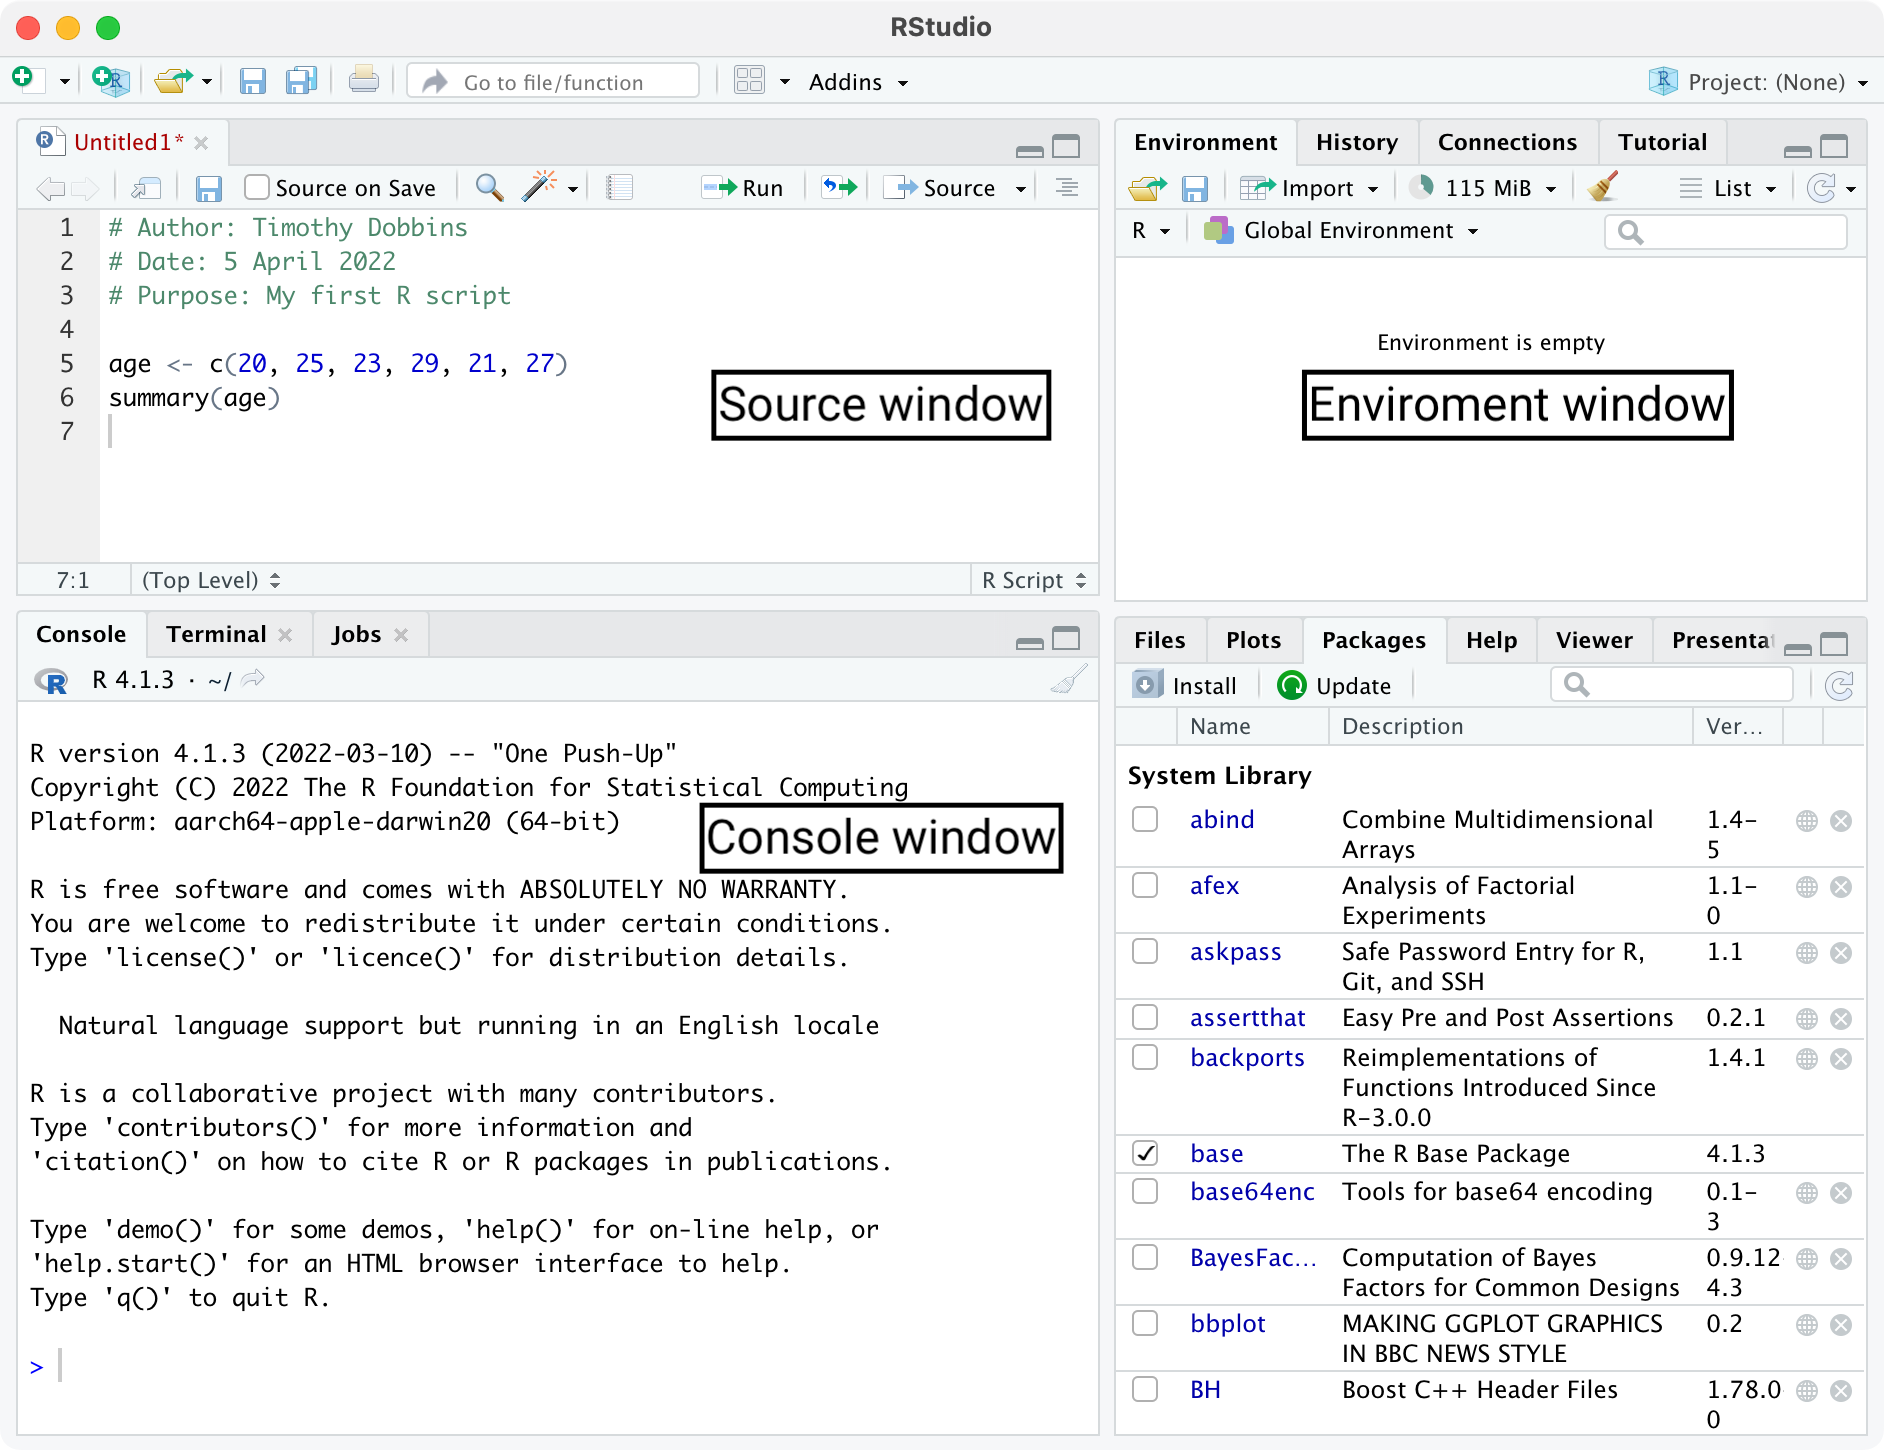
\includegraphics[width=1\linewidth]{img/RStudio-screenshot-03}

The \textbf{Source} window is where you will write and edit your R scripts. The R script can be saved by clicking on File -\textgreater{} Save As or by clicking on the symbol of a floppy disk at the top of the script. The file will have an extension of .R, for example name\_of\_script.R. Give it a meaningful title and remember to periodically save as you go.

In RStudio, the name of the script will be black when it has been saved, and will change to red if you have any unsaved changes.

The \textbf{Console} window, at the bottom left, contains the command line which is indicated with the symbol \textgreater. You can type commands here, but anything executed directly from the console is not saved and therefore is lost when the session ends (when you exit RStudio). You should always run your commands from a script file which you can save and use again later. When you run commands from a script, the output and any notes/errors are shown in the console. The Terminal and Jobs tabs will not be used in this course.

The \textbf{Environment} window at the top-right shows a list of objects that have been created during your session. When you close your RStudio session these objects will disappear. We will not use the History or Connections tabs in this course.

The bottom right corner contains some useful tabs, in particular the \textbf{Help} tab. When you are troubleshooting errors or learning how to use a function, the Help tab should be the first place you visit. Here you can search the help documents for all the packages you have installed. Whenever you create plots in R, these will be shown in the \textbf{Plots} tab. The \textbf{Packages} tab contains a list of installed packages and indicates which ones are currently in use (we will learn about packages later). Packages which are loaded, i.e.~in use, are indicated with a tick. Some packages are in use by default when you begin a new session. You can access information about a package by clicking on its name. The \textbf{Files} tab provides a shortcut to access your files. The Viewer tab will not be used in this course.

\hypertarget{some-r-basics}{%
\section{Some R basics}\label{some-r-basics}}

While we use R as a statistics package, R is a programming language. In order to use R effectively, we need to define some basics.

\hypertarget{objects}{%
\subsection{Objects}\label{objects}}

If you do some reading about R, you may learn that R is an ``object-oriented programming language''. When we enter or import data into R, we are asking R to create \textbf{objects} from our data. These objects can be manipulated and transformed by \textbf{functions}, to obtain useful insights from our data.

Objects in R are created using the \textbf{assignment operator}. The most common form of the assignment operator looks like an arrow: \texttt{\textless{}-} and is typed as the \texttt{\textless{}} and \texttt{-} symbols. The simplest way of reading \texttt{\textless{}-} is as the words ``is defined as''. Note that it possible to use \texttt{-\textgreater{}} and even \texttt{=} as assignment operators, but their use is less frequent.

Let's see an example:

\begin{Shaded}
\begin{Highlighting}[]
\NormalTok{x }\OtherTok{\textless{}{-}} \DecValTok{42}
\end{Highlighting}
\end{Shaded}

This command creates a new object called \texttt{x}, which is defined as the number 42 (or in words, ``\texttt{x} is defined as 42''). Running this command gives no output in the console, but the new object appears in the top-right \textbf{Environment} panel. We can view the object in the console by typing its name:

\begin{Shaded}
\begin{Highlighting}[]
\CommentTok{\# Print the object x}
\NormalTok{x}
\end{Highlighting}
\end{Shaded}

\begin{verbatim}
## [1] 42
\end{verbatim}

Now we see the contents of \texttt{x} in the console.

This example is rather trivial, and we rarely assign objects of just one value. We'll see a more realistic example soon.

\hypertarget{data-structures}{%
\subsection{Data structures}\label{data-structures}}

There are two main data structures we will use in the course: \textbf{vectors} and \textbf{data frames}. A \textbf{vector} is a combination of data values, all of the same type. For example, our six ages that we entered earlier is a vector. You could think of a vector as a column of data (even though R prints vectors as rows!) And technically, even an object with only one value is a vector, a vector of size 1.

The easiest way of creating a vector in R is by using the \texttt{c()} function, where c stands for `combine'. In our previous Simple Analysis in R (Section \ref{simpleR}), we wrote the command:

\begin{Shaded}
\begin{Highlighting}[]
\NormalTok{age }\OtherTok{\textless{}{-}} \FunctionTok{c}\NormalTok{(}\DecValTok{20}\NormalTok{, }\DecValTok{25}\NormalTok{, }\DecValTok{23}\NormalTok{, }\DecValTok{29}\NormalTok{, }\DecValTok{21}\NormalTok{, }\DecValTok{27}\NormalTok{)}
\end{Highlighting}
\end{Shaded}

This command created a new object called \texttt{age}, and \emph{combined} the six values of age into one vector.

Just as having a vector of size 1 is unusual, having just one column of data to analyse is also pretty unusual. The other structure we will describe here is a \textbf{data frame} which is essentially a collection of vectors, each of the same size. You could think of a data frame as being like a spreadsheet, with columns representing variables, and rows representing observations.

There are other structures in R, such as matrices and lists, which we won't discuss in this course.

\hypertarget{functions}{%
\subsection{Functions}\label{functions}}

If objects are the nouns of R, functions are the verbs. Essentially, functions transform objects. Functions can transform your data into summary statistics, graphical summaries or analysis results. For example, we used the \texttt{summary()} function to display summary statistics for our six ages.

R functions are specified by their arguments (or inputs). The arguments that can be supplied for each function can be inspected by examining the help notes for that function. To obtain help for a function, we can submit \texttt{help(summary)} (or equivalently \texttt{?summary()}) in the console, or we can use the \textbf{help} tab in the bottom-right window of RStudio. For example, the first part of the help notes for \texttt{summary} appear as:

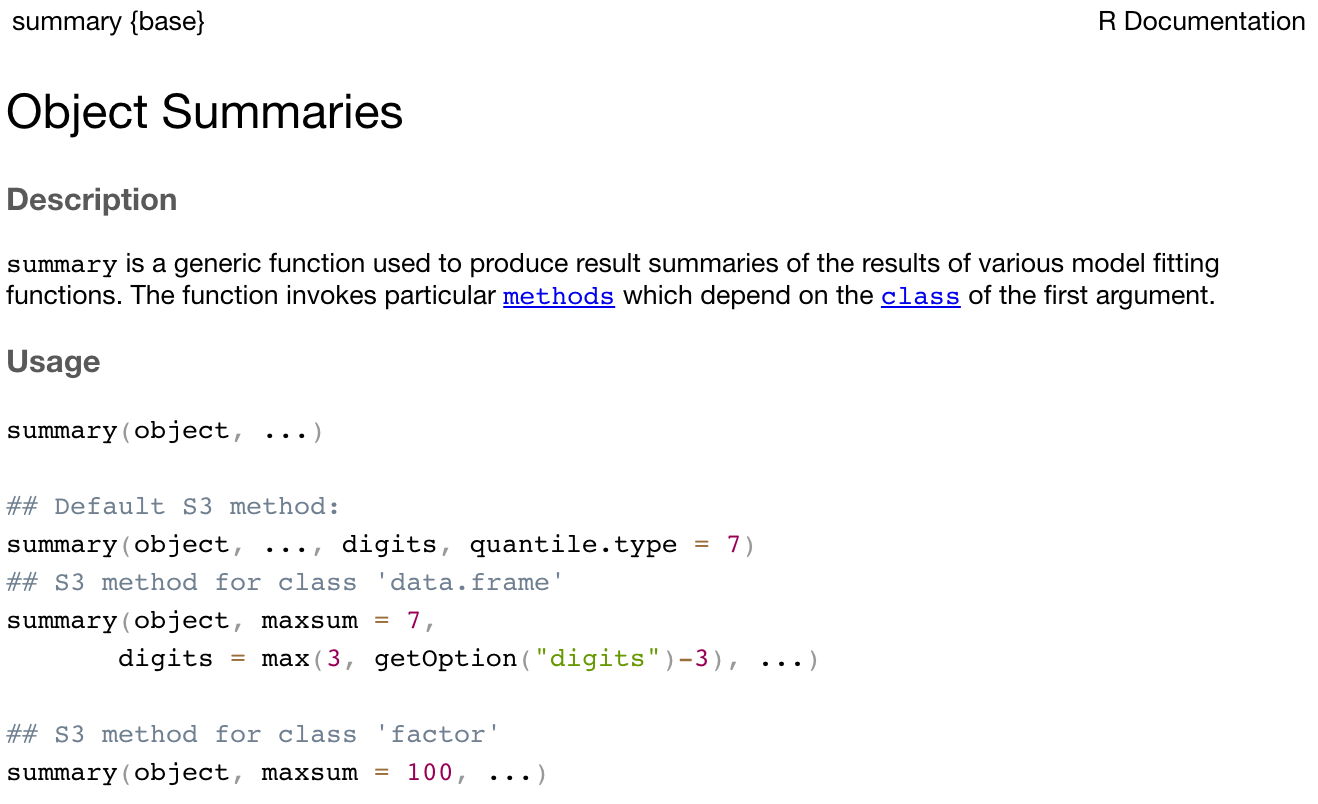
\includegraphics[width=0.8\linewidth]{img/help-1}

The help notes in R can be quite cryptic, but \textbf{Usage} section details what values should be provided for the function to run. Here, \texttt{summary} requires an object to be specified. In our case, we specified \texttt{age}, which is our object defined as the vector of six ages.

Most help pages also include some examples of how you might use the function. These can be found at the very bottom of the help page.

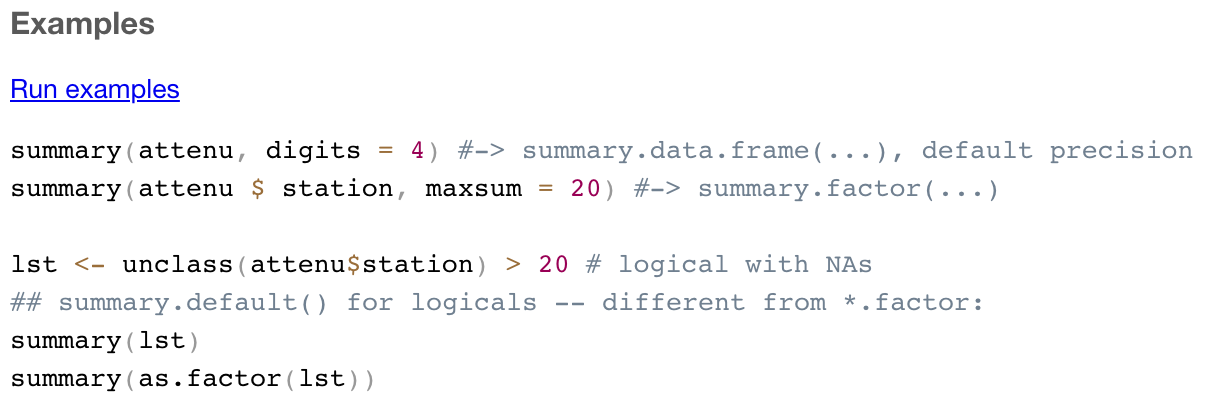
\includegraphics[width=0.8\linewidth]{img/help-2}

The \texttt{summary} function is quite simple, in that it only requires one input, the object to be summarised. More complex functions might require a number of inputs. For example, the help notes for the \texttt{descriptives()} function in the \texttt{jmv} package show a large number of inputs can be specified:

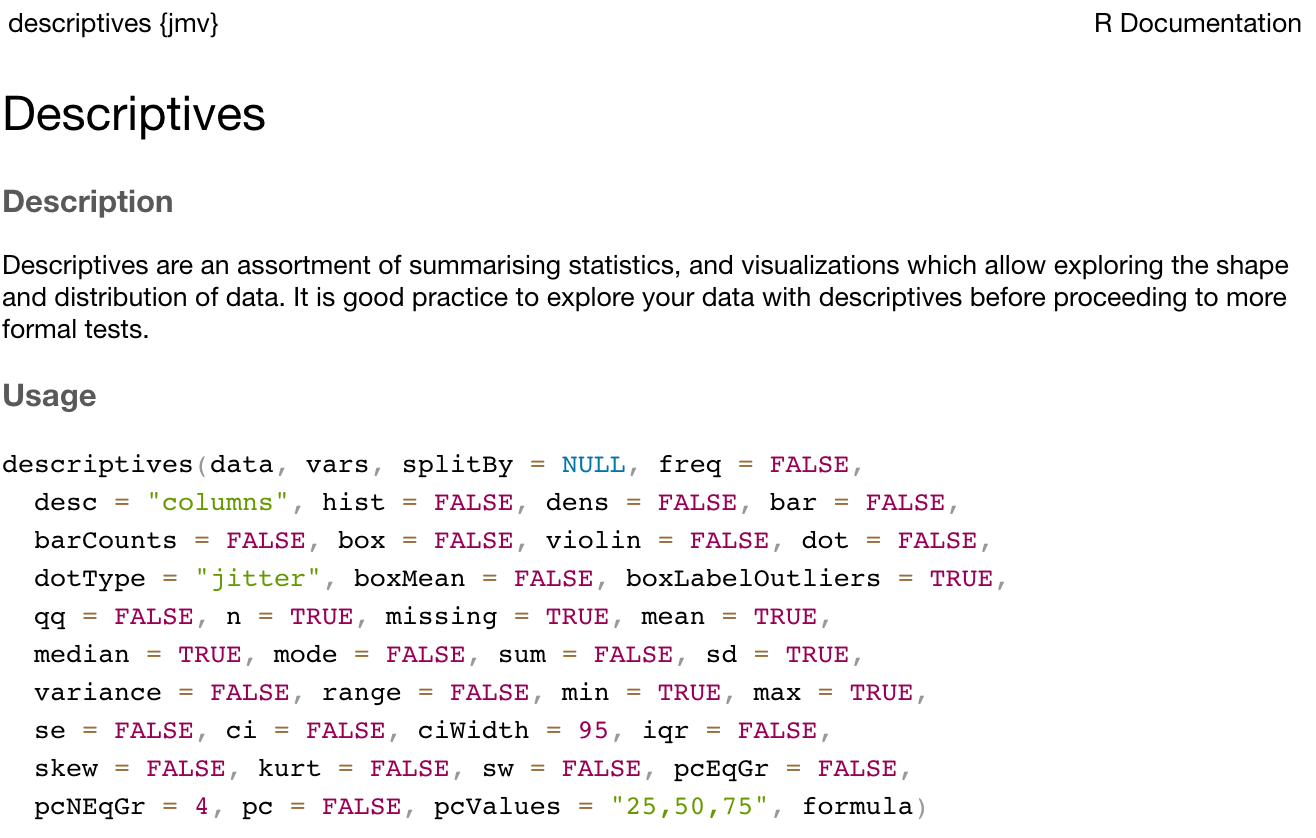
\includegraphics[width=0.8\linewidth]{img/help-3}

There are two things to note here. First, notice that the first two inputs are listed with no = symbol, but all other inputs are listed with = symbols (with values provided after the = symbol). This means that everything apart from \texttt{data} and \texttt{vars} have \textbf{default} values. We are free to not include values for these inputs if we are happy with the defaults provided. For example, by default the variance is not calculated (as \texttt{variance\ =\ FALSE}). To obtain the variance as well as the standard deviation, we can change this default to \texttt{variance\ =\ TRUE}:

\begin{Shaded}
\begin{Highlighting}[]
\CommentTok{\# Only the standard deviation is provided as the measure of variability}
\FunctionTok{descriptives}\NormalTok{(}\AttributeTok{data=}\NormalTok{pbc, }\AttributeTok{vars=}\NormalTok{age)}

\CommentTok{\# Additionally request the variance to be calculated}
\FunctionTok{descriptives}\NormalTok{(}\AttributeTok{data=}\NormalTok{pbc, }\AttributeTok{vars=}\NormalTok{age, }\AttributeTok{variance=}\ConstantTok{TRUE}\NormalTok{)}
\end{Highlighting}
\end{Shaded}

Second, for functions with multiple inputs, we can specify the input name and its value, or we can specify the inputs \textbf{in the order listed in the Usage section}. So the following are equivalent:

\begin{Shaded}
\begin{Highlighting}[]
\CommentTok{\# We can specify that the dataset to be summarised is pbc,}
\CommentTok{\#   and the variable to summarise is age:}
\FunctionTok{descriptives}\NormalTok{(}\AttributeTok{data=}\NormalTok{pbc, }\AttributeTok{vars=}\NormalTok{age)}

\CommentTok{\# We can omit the input name, as long as we keep the inputs in the correct order {-} }
\CommentTok{\#   that is, dataset first, variable second:}
\FunctionTok{descriptives}\NormalTok{(pbc, age)}

\CommentTok{\# We can change the order of the inputs, as long as we specify the input name:}
\FunctionTok{descriptives}\NormalTok{(}\AttributeTok{vars=}\NormalTok{age, }\AttributeTok{data=}\NormalTok{pbc)}
\end{Highlighting}
\end{Shaded}

In this course, we will usually provide all the input names, even when they are not required.

\hypertarget{packages}{%
\subsection{Packages}\label{packages}}

A \textbf{package} is a collection of functions, documentation (and sometimes datasets) that extend the capabilities of R. Packages have been written by R users to be freely distributed and used by others. R packages can be obtained from many sources, but the most common source is CRAN: the Comprehensive R Archive Network.

A useful way of thinking about R is that R is like a smartphone, with packages being like apps which are downloaded from CRAN (similar to an app-store). When you first install R, it comes with a basic set of packages (apps) installed. You can do a lot of things with these basic packages, but sometimes you might want to do things differently (you might prefer Firefox as your browser), or you may want to perform some analyses that can't be done using the default packages. In these cases, you can install a package.

Like installing an app on a smartphone, you only need to \emph{install} a package once. But each time you want to use the package, you need to \emph{load} the package into R. This is similar to running the app on your phone. The analogy falls down a bit in that we usually load more than one package in an R script - but we only load the packages we need for that R session.

\hypertarget{how-to-install-a-package}{%
\subsection{How to install a package}\label{how-to-install-a-package}}

There are a couple of ways to install a package. You can use the \texttt{install.packages()} function if you know the exact name of the package. Let's use an example of installing the \texttt{skimr} package, which gives a very nice, high-level overview of any data frame. We can install \texttt{skimr} by typing the following into the console:

\begin{Shaded}
\begin{Highlighting}[]
\FunctionTok{install.packages}\NormalTok{(}\StringTok{"skimr"}\NormalTok{)}
\end{Highlighting}
\end{Shaded}

Note the use of the quotation marks.

Alternatively, RStudio offers a graphical way of installing packages that can be accessed via \textbf{Tools \textgreater{} Install Packages}, or via the \textbf{Install} button at the top of the \textbf{Packages} tab in the bottom-right window. You can begin typing the name of the package in the dialog box that appears, and RStudio will use predictive text to offer possible packages:

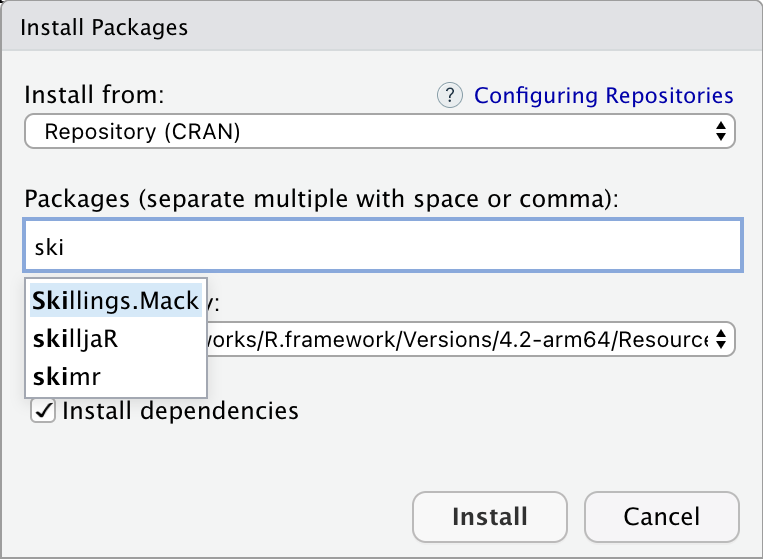
\includegraphics[width=0.6\linewidth]{img/install-packages}

While writing code is usually the recommended way to use R, installing packages is an exception. Using the graphical interface is perfectly fine, because you only need to install a package once.

\hypertarget{how-to-load-a-package}{%
\subsection{How to load a package}\label{how-to-load-a-package}}

When you begin a new session in RStudio, i.e.~when you open RStudio, only certain core packages are automatically loaded. You can use the \texttt{library()} function to load a package that you has previously been installed. For example, now that we have installed \texttt{skimr}, we need to load it before we can use it:

\begin{Shaded}
\begin{Highlighting}[]
\FunctionTok{library}\NormalTok{(skimr)}
\end{Highlighting}
\end{Shaded}

Note that quotation marks are not required for the \texttt{library()} function (although they can be included if you really like quotation marks!).

\hypertarget{part-2-obtaining-basic-descriptive-statistics}{%
\section{Part 2: Obtaining basic descriptive statistics}\label{part-2-obtaining-basic-descriptive-statistics}}

In this exercise, we will analyse data to complete a descriptive table from a research study. The data come from a study in primary biliary cirrhosis, a condition of the liver, from \citet{therneau_grambsch10}, Modeling Survival Data: Extending the Cox Model. By the end of this exercise, we will have completed the following table.

 
  \providecommand{\huxb}[2]{\arrayrulecolor[RGB]{#1}\global\arrayrulewidth=#2pt}
  \providecommand{\huxvb}[2]{\color[RGB]{#1}\vrule width #2pt}
  \providecommand{\huxtpad}[1]{\rule{0pt}{#1}}
  \providecommand{\huxbpad}[1]{\rule[-#1]{0pt}{#1}}

\begin{table}[ht]
\begin{centerbox}
\begin{threeparttable}
\captionsetup{justification=centering,singlelinecheck=off}
\caption{\label{tab:unnamed-chunk-18} Summary of 418 participants from the PBC study (Therneau and Grambsch, 2000)}
 \setlength{\tabcolsep}{0pt}
\begin{tabularx}{0.95\textwidth}{p{0.316666666666667\textwidth} p{0.316666666666667\textwidth} p{0.316666666666667\textwidth}}


\hhline{>{\huxb{0, 0, 0}{0.4}}->{\huxb{0, 0, 0}{0.4}}->{\huxb{0, 0, 0}{0.4}}-}
\arrayrulecolor{black}

\multicolumn{1}{!{\huxvb{0, 0, 0}{0}}p{0.316666666666667\textwidth}!{\huxvb{0, 0, 0}{0}}}{\hspace{0pt}\parbox[b]{0.316666666666667\textwidth-0pt-6pt}{\huxtpad{6pt + 1em}\raggedright \textbf{Characteristic}\huxbpad{6pt}}} &
\multicolumn{1}{p{0.316666666666667\textwidth}!{\huxvb{0, 0, 0}{0}}}{\hspace{6pt}\parbox[b]{0.316666666666667\textwidth-6pt-6pt}{\huxtpad{6pt + 1em}\raggedright \textbf{ }\huxbpad{6pt}}} &
\multicolumn{1}{p{0.316666666666667\textwidth}!{\huxvb{0, 0, 0}{0}}}{\hspace{6pt}\parbox[b]{0.316666666666667\textwidth-6pt-0pt}{\huxtpad{6pt + 1em}\raggedright \textbf{Summary}\huxbpad{6pt}}} \tabularnewline[-0.5pt]


\hhline{>{\huxb{0, 0, 0}{0.4}}->{\huxb{0, 0, 0}{0.4}}->{\huxb{0, 0, 0}{0.4}}-}
\arrayrulecolor{black}

\multicolumn{1}{!{\huxvb{0, 0, 0}{0}}p{0.316666666666667\textwidth}!{\huxvb{0, 0, 0}{0}}}{\hspace{0pt}\parbox[b]{0.316666666666667\textwidth-0pt-6pt}{\huxtpad{6pt + 1em}\raggedright Age (years)\huxbpad{6pt}}} &
\multicolumn{1}{p{0.316666666666667\textwidth}!{\huxvb{0, 0, 0}{0}}}{\hspace{6pt}\parbox[b]{0.316666666666667\textwidth-6pt-6pt}{\huxtpad{6pt + 1em}\raggedright \huxbpad{6pt}}} &
\multicolumn{1}{p{0.316666666666667\textwidth}!{\huxvb{0, 0, 0}{0}}}{\hspace{6pt}\parbox[b]{0.316666666666667\textwidth-6pt-0pt}{\huxtpad{6pt + 1em}\raggedright Mean (SD) or Median [IQR]\huxbpad{6pt}}} \tabularnewline[-0.5pt]


\hhline{}
\arrayrulecolor{black}

\multicolumn{1}{!{\huxvb{0, 0, 0}{0}}p{0.316666666666667\textwidth}!{\huxvb{0, 0, 0}{0}}}{} &
\multicolumn{1}{p{0.316666666666667\textwidth}!{\huxvb{0, 0, 0}{0}}}{\hspace{6pt}\parbox[b]{0.316666666666667\textwidth-6pt-6pt}{\huxtpad{6pt + 1em}\raggedright Male\huxbpad{6pt}}} &
\multicolumn{1}{p{0.316666666666667\textwidth}!{\huxvb{0, 0, 0}{0}}}{\hspace{6pt}\parbox[b]{0.316666666666667\textwidth-6pt-0pt}{\huxtpad{6pt + 1em}\raggedright n (\%)\huxbpad{6pt}}} \tabularnewline[-0.5pt]


\hhline{}
\arrayrulecolor{black}

\multicolumn{1}{!{\huxvb{0, 0, 0}{0}}p{0.316666666666667\textwidth}!{\huxvb{0, 0, 0}{0}}}{\multirow[t]{-2}{*}[0ex]{\hspace{0pt}\parbox[b]{0.316666666666667\textwidth-0pt-6pt}{\huxtpad{6pt + 1em}\raggedright Sex\huxbpad{6pt}}}} &
\multicolumn{1}{p{0.316666666666667\textwidth}!{\huxvb{0, 0, 0}{0}}}{\hspace{6pt}\parbox[b]{0.316666666666667\textwidth-6pt-6pt}{\huxtpad{6pt + 1em}\raggedright Female\huxbpad{6pt}}} &
\multicolumn{1}{p{0.316666666666667\textwidth}!{\huxvb{0, 0, 0}{0}}}{\hspace{6pt}\parbox[b]{0.316666666666667\textwidth-6pt-0pt}{\huxtpad{6pt + 1em}\raggedright n (\%)\huxbpad{6pt}}} \tabularnewline[-0.5pt]


\hhline{}
\arrayrulecolor{black}

\multicolumn{1}{!{\huxvb{0, 0, 0}{0}}p{0.316666666666667\textwidth}!{\huxvb{0, 0, 0}{0}}}{\hspace{0pt}\parbox[b]{0.316666666666667\textwidth-0pt-6pt}{\huxtpad{6pt + 1em}\raggedright AST* (U/ml)\huxbpad{6pt}}} &
\multicolumn{1}{p{0.316666666666667\textwidth}!{\huxvb{0, 0, 0}{0}}}{\hspace{6pt}\parbox[b]{0.316666666666667\textwidth-6pt-6pt}{\huxtpad{6pt + 1em}\raggedright \huxbpad{6pt}}} &
\multicolumn{1}{p{0.316666666666667\textwidth}!{\huxvb{0, 0, 0}{0}}}{\hspace{6pt}\parbox[b]{0.316666666666667\textwidth-6pt-0pt}{\huxtpad{6pt + 1em}\raggedright Mean (SD) or Median [IQR]\huxbpad{6pt}}} \tabularnewline[-0.5pt]


\hhline{}
\arrayrulecolor{black}

\multicolumn{1}{!{\huxvb{0, 0, 0}{0}}p{0.316666666666667\textwidth}!{\huxvb{0, 0, 0}{0}}}{\hspace{0pt}\parbox[b]{0.316666666666667\textwidth-0pt-6pt}{\huxtpad{6pt + 1em}\raggedright Serum bilirubin\huxbpad{6pt}}} &
\multicolumn{1}{p{0.316666666666667\textwidth}!{\huxvb{0, 0, 0}{0}}}{\hspace{6pt}\parbox[b]{0.316666666666667\textwidth-6pt-6pt}{\huxtpad{6pt + 1em}\raggedright \huxbpad{6pt}}} &
\multicolumn{1}{p{0.316666666666667\textwidth}!{\huxvb{0, 0, 0}{0}}}{\hspace{6pt}\parbox[b]{0.316666666666667\textwidth-6pt-0pt}{\huxtpad{6pt + 1em}\raggedright Mean (SD) or Median [IQR]\huxbpad{6pt}}} \tabularnewline[-0.5pt]


\hhline{}
\arrayrulecolor{black}

\multicolumn{1}{!{\huxvb{0, 0, 0}{0}}p{0.316666666666667\textwidth}!{\huxvb{0, 0, 0}{0}}}{} &
\multicolumn{1}{p{0.316666666666667\textwidth}!{\huxvb{0, 0, 0}{0}}}{\hspace{6pt}\parbox[b]{0.316666666666667\textwidth-6pt-6pt}{\huxtpad{6pt + 1em}\raggedright I\huxbpad{6pt}}} &
\multicolumn{1}{p{0.316666666666667\textwidth}!{\huxvb{0, 0, 0}{0}}}{\hspace{6pt}\parbox[b]{0.316666666666667\textwidth-6pt-0pt}{\huxtpad{6pt + 1em}\raggedright n (\%)\huxbpad{6pt}}} \tabularnewline[-0.5pt]


\hhline{}
\arrayrulecolor{black}

\multicolumn{1}{!{\huxvb{0, 0, 0}{0}}p{0.316666666666667\textwidth}!{\huxvb{0, 0, 0}{0}}}{} &
\multicolumn{1}{p{0.316666666666667\textwidth}!{\huxvb{0, 0, 0}{0}}}{\hspace{6pt}\parbox[b]{0.316666666666667\textwidth-6pt-6pt}{\huxtpad{6pt + 1em}\raggedright II\huxbpad{6pt}}} &
\multicolumn{1}{p{0.316666666666667\textwidth}!{\huxvb{0, 0, 0}{0}}}{\hspace{6pt}\parbox[b]{0.316666666666667\textwidth-6pt-0pt}{\huxtpad{6pt + 1em}\raggedright n (\%)\huxbpad{6pt}}} \tabularnewline[-0.5pt]


\hhline{}
\arrayrulecolor{black}

\multicolumn{1}{!{\huxvb{0, 0, 0}{0}}p{0.316666666666667\textwidth}!{\huxvb{0, 0, 0}{0}}}{} &
\multicolumn{1}{p{0.316666666666667\textwidth}!{\huxvb{0, 0, 0}{0}}}{\hspace{6pt}\parbox[b]{0.316666666666667\textwidth-6pt-6pt}{\huxtpad{6pt + 1em}\raggedright III\huxbpad{6pt}}} &
\multicolumn{1}{p{0.316666666666667\textwidth}!{\huxvb{0, 0, 0}{0}}}{\hspace{6pt}\parbox[b]{0.316666666666667\textwidth-6pt-0pt}{\huxtpad{6pt + 1em}\raggedright n (\%)\huxbpad{6pt}}} \tabularnewline[-0.5pt]


\hhline{}
\arrayrulecolor{black}

\multicolumn{1}{!{\huxvb{0, 0, 0}{0}}p{0.316666666666667\textwidth}!{\huxvb{0, 0, 0}{0}}}{\multirow[t]{-4}{*}[0ex]{\hspace{0pt}\parbox[b]{0.316666666666667\textwidth-0pt-6pt}{\huxtpad{6pt + 1em}\raggedright Stage\huxbpad{6pt}}}} &
\multicolumn{1}{p{0.316666666666667\textwidth}!{\huxvb{0, 0, 0}{0}}}{\hspace{6pt}\parbox[b]{0.316666666666667\textwidth-6pt-6pt}{\huxtpad{6pt + 1em}\raggedright IIIV\huxbpad{6pt}}} &
\multicolumn{1}{p{0.316666666666667\textwidth}!{\huxvb{0, 0, 0}{0}}}{\hspace{6pt}\parbox[b]{0.316666666666667\textwidth-6pt-0pt}{\huxtpad{6pt + 1em}\raggedright n (\%)\huxbpad{6pt}}} \tabularnewline[-0.5pt]


\hhline{}
\arrayrulecolor{black}

\multicolumn{1}{!{\huxvb{0, 0, 0}{0}}p{0.316666666666667\textwidth}!{\huxvb{0, 0, 0}{0}}}{} &
\multicolumn{1}{p{0.316666666666667\textwidth}!{\huxvb{0, 0, 0}{0}}}{\hspace{6pt}\parbox[b]{0.316666666666667\textwidth-6pt-6pt}{\huxtpad{6pt + 1em}\raggedright Alive: no transplant\huxbpad{6pt}}} &
\multicolumn{1}{p{0.316666666666667\textwidth}!{\huxvb{0, 0, 0}{0}}}{\hspace{6pt}\parbox[b]{0.316666666666667\textwidth-6pt-0pt}{\huxtpad{6pt + 1em}\raggedright n (\%)\huxbpad{6pt}}} \tabularnewline[-0.5pt]


\hhline{}
\arrayrulecolor{black}

\multicolumn{1}{!{\huxvb{0, 0, 0}{0}}p{0.316666666666667\textwidth}!{\huxvb{0, 0, 0}{0}}}{} &
\multicolumn{1}{p{0.316666666666667\textwidth}!{\huxvb{0, 0, 0}{0}}}{\hspace{6pt}\parbox[b]{0.316666666666667\textwidth-6pt-6pt}{\huxtpad{6pt + 1em}\raggedright Alive: transplant\huxbpad{6pt}}} &
\multicolumn{1}{p{0.316666666666667\textwidth}!{\huxvb{0, 0, 0}{0}}}{\hspace{6pt}\parbox[b]{0.316666666666667\textwidth-6pt-0pt}{\huxtpad{6pt + 1em}\raggedright n (\%)\huxbpad{6pt}}} \tabularnewline[-0.5pt]


\hhline{}
\arrayrulecolor{black}

\multicolumn{1}{!{\huxvb{0, 0, 0}{0}}p{0.316666666666667\textwidth}!{\huxvb{0, 0, 0}{0}}}{\multirow[t]{-3}{*}[0ex]{\hspace{0pt}\parbox[b]{0.316666666666667\textwidth-0pt-6pt}{\huxtpad{6pt + 1em}\raggedright Vital status at study end\huxbpad{6pt}}}} &
\multicolumn{1}{p{0.316666666666667\textwidth}!{\huxvb{0, 0, 0}{0}}}{\hspace{6pt}\parbox[b]{0.316666666666667\textwidth-6pt-6pt}{\huxtpad{6pt + 1em}\raggedright Deceased\huxbpad{6pt}}} &
\multicolumn{1}{p{0.316666666666667\textwidth}!{\huxvb{0, 0, 0}{0}}}{\hspace{6pt}\parbox[b]{0.316666666666667\textwidth-6pt-0pt}{\huxtpad{6pt + 1em}\raggedright n (\%)\huxbpad{6pt}}} \tabularnewline[-0.5pt]


\hhline{>{\huxb{0, 0, 0}{0.8}}->{\huxb{0, 0, 0}{0.8}}->{\huxb{0, 0, 0}{0.8}}-}
\arrayrulecolor{black}

\multicolumn{3}{!{\huxvb{0, 0, 0}{0}}p{0.95\textwidth+4\tabcolsep}!{\huxvb{0, 0, 0}{0}}}{\hspace{6pt}\parbox[b]{0.95\textwidth+4\tabcolsep-6pt-6pt}{\huxtpad{6pt + 1em}\raggedright * asparate aminotransferase\huxbpad{6pt}}} \tabularnewline[-0.5pt]


\hhline{}
\arrayrulecolor{black}
\end{tabularx}
\end{threeparttable}\par\end{centerbox}

\end{table}
 

This table is available in Table1.docx, saved on Moodle.

\hypertarget{opening-a-data-file}{%
\subsection{Opening a data file}\label{opening-a-data-file}}

Typing data directly into R is not common; we usually open data that have been previously saved. There are two useful packages for importing data into R: \texttt{haven} (for data that have been saved by Stata, SAS or SPSS) and \texttt{readxl} (for data saved by Microsoft Excel). Additionally, the \texttt{labelled} package is useful in working with data that have been labelled in Stata. Here, we will open a dataset that has been stored as a Stata data file (which has the .dta suffix):

1 - If necessary, install the \texttt{haven} and \texttt{readxl} packages. As mentioned earlier, packages only need to be installed if they have not been installed earlier.

\begin{Shaded}
\begin{Highlighting}[]
\FunctionTok{install.packages}\NormalTok{(}\StringTok{"haven"}\NormalTok{)}
\FunctionTok{install.packages}\NormalTok{(}\StringTok{"readxl"}\NormalTok{)}
\end{Highlighting}
\end{Shaded}

2 - Locate the data set called pbc.dta on Moodle. Click the file to download it, and then save it in a folder you will be able to locate later - for example, your OneDrive folder. The description of this dataset (i.e.~the metadata) have been saved as a plain text file: pbc\_info.txt. Locate the file and filepath of pbc.dta.

3 - In R, use the \texttt{read\_dta()} function to read the Stata data into new object called \texttt{pbc}. Remember that we need to load the \texttt{haven} and \texttt{labelled} packages into R:

\begin{Shaded}
\begin{Highlighting}[]
\FunctionTok{library}\NormalTok{(haven)}
\FunctionTok{library}\NormalTok{(labelled)}
\FunctionTok{library}\NormalTok{(skimr)}

\NormalTok{pbc }\OtherTok{\textless{}{-}} \FunctionTok{read\_dta}\NormalTok{(}\StringTok{"data/examples/pbc.dta"}\NormalTok{)}
\end{Highlighting}
\end{Shaded}

4 - We now re-assign the pbc object by using the \texttt{unlabelled()} function from the \texttt{labelled} package:

\begin{Shaded}
\begin{Highlighting}[]
\NormalTok{pbc }\OtherTok{\textless{}{-}} \FunctionTok{unlabelled}\NormalTok{(pbc)}
\end{Highlighting}
\end{Shaded}

Note that we can combine the \texttt{unlabelled()} and \texttt{read\_dta()} functions together, to complete this process in one line:

\begin{Shaded}
\begin{Highlighting}[]
\NormalTok{pbc }\OtherTok{\textless{}{-}} \FunctionTok{unlabelled}\NormalTok{(}\FunctionTok{read\_dta}\NormalTok{(}\StringTok{"data/examples/pbc.dta"}\NormalTok{))}
\end{Highlighting}
\end{Shaded}

5 - We can now use the \texttt{summary()} function to examine the pbc dataset.

\begin{Shaded}
\begin{Highlighting}[]
\FunctionTok{summary}\NormalTok{(pbc)}
\end{Highlighting}
\end{Shaded}

\begin{verbatim}
##        id             time          status            trt       
##  Min.   :  1.0   Min.   :  41   Min.   :0.0000   Min.   :1.000  
##  1st Qu.:105.2   1st Qu.:1093   1st Qu.:0.0000   1st Qu.:1.000  
##  Median :209.5   Median :1730   Median :0.0000   Median :1.000  
##  Mean   :209.5   Mean   :1918   Mean   :0.8301   Mean   :1.494  
##  3rd Qu.:313.8   3rd Qu.:2614   3rd Qu.:2.0000   3rd Qu.:2.000  
##  Max.   :418.0   Max.   :4795   Max.   :2.0000   Max.   :2.000  
##                                                  NA's   :106    
##       age             sex           ascites            hepato      
##  Min.   :26.28   Min.   :1.000   Min.   :0.00000   Min.   :0.0000  
##  1st Qu.:42.83   1st Qu.:2.000   1st Qu.:0.00000   1st Qu.:0.0000  
##  Median :51.00   Median :2.000   Median :0.00000   Median :1.0000  
##  Mean   :50.74   Mean   :1.895   Mean   :0.07692   Mean   :0.5128  
##  3rd Qu.:58.24   3rd Qu.:2.000   3rd Qu.:0.00000   3rd Qu.:1.0000  
##  Max.   :78.44   Max.   :2.000   Max.   :1.00000   Max.   :1.0000  
##                                  NA's   :106       NA's   :106     
##     spiders           edema             bili             chol       
##  Min.   :0.0000   Min.   :0.0000   Min.   : 0.300   Min.   : 120.0  
##  1st Qu.:0.0000   1st Qu.:0.0000   1st Qu.: 0.800   1st Qu.: 249.5  
##  Median :0.0000   Median :0.0000   Median : 1.400   Median : 309.5  
##  Mean   :0.2885   Mean   :0.1005   Mean   : 3.221   Mean   : 369.5  
##  3rd Qu.:1.0000   3rd Qu.:0.0000   3rd Qu.: 3.400   3rd Qu.: 400.0  
##  Max.   :1.0000   Max.   :1.0000   Max.   :28.000   Max.   :1775.0  
##  NA's   :106                                        NA's   :134     
##     albumin          copper          alkphos             ast        
##  Min.   :1.960   Min.   :  4.00   Min.   :  289.0   Min.   : 26.35  
##  1st Qu.:3.243   1st Qu.: 41.25   1st Qu.:  871.5   1st Qu.: 80.60  
##  Median :3.530   Median : 73.00   Median : 1259.0   Median :114.70  
##  Mean   :3.497   Mean   : 97.65   Mean   : 1982.7   Mean   :122.56  
##  3rd Qu.:3.770   3rd Qu.:123.00   3rd Qu.: 1980.0   3rd Qu.:151.90  
##  Max.   :4.640   Max.   :588.00   Max.   :13862.4   Max.   :457.25  
##                  NA's   :108      NA's   :106       NA's   :106     
##       trig           platelet        protime          stage      
##  Min.   : 33.00   Min.   : 62.0   Min.   : 9.00   Min.   :1.000  
##  1st Qu.: 84.25   1st Qu.:188.5   1st Qu.:10.00   1st Qu.:2.000  
##  Median :108.00   Median :251.0   Median :10.60   Median :3.000  
##  Mean   :124.70   Mean   :257.0   Mean   :10.73   Mean   :3.024  
##  3rd Qu.:151.00   3rd Qu.:318.0   3rd Qu.:11.10   3rd Qu.:4.000  
##  Max.   :598.00   Max.   :721.0   Max.   :18.00   Max.   :4.000  
##  NA's   :136      NA's   :11      NA's   :2       NA's   :6
\end{verbatim}

An alternative to the \texttt{summary()} function is the \texttt{skim()} function in the \texttt{skimr} package, which produces summary statistics as well as rudimentary histograms:

\begin{Shaded}
\begin{Highlighting}[]
\FunctionTok{skim}\NormalTok{(pbc)}
\end{Highlighting}
\end{Shaded}

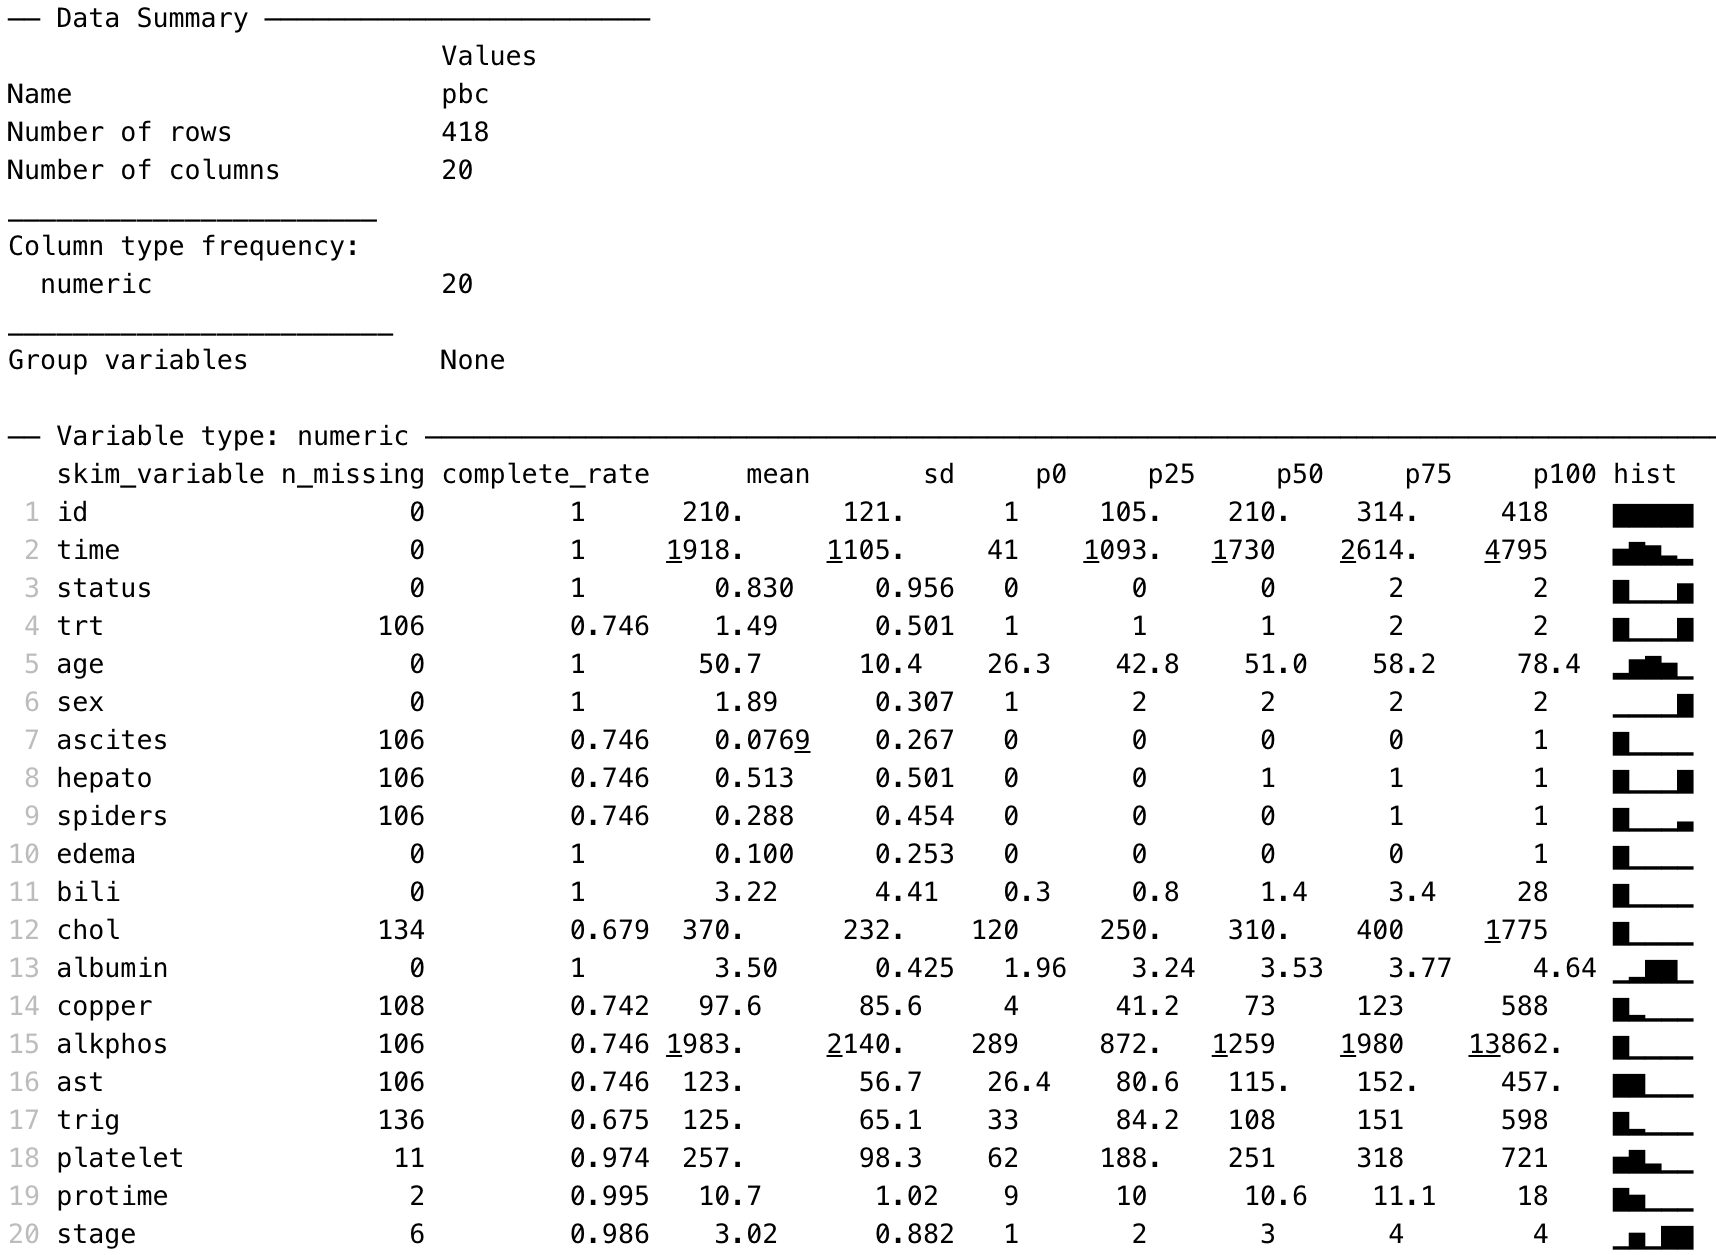
\includegraphics[width=0.9\linewidth]{img/skim-pbc}

\hypertarget{summarising-continuous-variables}{%
\subsection{Summarising continuous variables}\label{summarising-continuous-variables}}

One of the most flexible functions for summarising continuous variables is the \texttt{descriptives()} function from the \texttt{jmv} package. The function is specified as \texttt{descriptives(data=,\ vars=)} where:

\begin{itemize}
\tightlist
\item
  \texttt{data} specifies the dataframe to be analysed
\item
  \texttt{vars} specifies the variable(s) of interest, with multiple variables combined using the \texttt{c()} function
\end{itemize}

We can summarise the three continuous variables in the pbc data: age, AST and serum bilirubin, as shown below.

\begin{Shaded}
\begin{Highlighting}[]
\FunctionTok{library}\NormalTok{(jmv)}

\FunctionTok{descriptives}\NormalTok{(}\AttributeTok{data=}\NormalTok{pbc, }\AttributeTok{vars=}\FunctionTok{c}\NormalTok{(age, ast, bili))}
\end{Highlighting}
\end{Shaded}

\begin{verbatim}
## 
##  DESCRIPTIVES
## 
##  Descriptives                                                
##  ─────────────────────────────────────────────────────────── 
##                          age         ast         bili        
##  ─────────────────────────────────────────────────────────── 
##    N                          418         312          418   
##    Missing                      0         106            0   
##    Mean                  50.74155    122.5563     3.220813   
##    Median                51.00068    114.7000     1.400000   
##    Standard deviation    10.44721    56.69952     4.407506   
##    Minimum               26.27789    26.35000    0.3000000   
##    Maximum               78.43943    457.2500     28.00000   
##  ───────────────────────────────────────────────────────────
\end{verbatim}

By default, the \texttt{descriptives} function presents the mean, median, standard deviation, minimum and maximum. We can request additional statistics, such as the quartiles (which are called the percentiles, or pc, in the descriptives function):

\begin{Shaded}
\begin{Highlighting}[]
\FunctionTok{descriptives}\NormalTok{(}\AttributeTok{data=}\NormalTok{pbc, }\AttributeTok{vars=}\FunctionTok{c}\NormalTok{(age, ast, bili), }\AttributeTok{pc=}\ConstantTok{TRUE}\NormalTok{)}
\end{Highlighting}
\end{Shaded}

\begin{verbatim}
## 
##  DESCRIPTIVES
## 
##  Descriptives                                                
##  ─────────────────────────────────────────────────────────── 
##                          age         ast         bili        
##  ─────────────────────────────────────────────────────────── 
##    N                          418         312          418   
##    Missing                      0         106            0   
##    Mean                  50.74155    122.5563     3.220813   
##    Median                51.00068    114.7000     1.400000   
##    Standard deviation    10.44721    56.69952     4.407506   
##    Minimum               26.27789    26.35000    0.3000000   
##    Maximum               78.43943    457.2500     28.00000   
##    25th percentile       42.83231    80.60000    0.8000000   
##    50th percentile       51.00068    114.7000     1.400000   
##    75th percentile       58.24093    151.9000     3.400000   
##  ───────────────────────────────────────────────────────────
\end{verbatim}

\hypertarget{producing-a-histogram}{%
\subsection{Producing a histogram}\label{producing-a-histogram}}

We can use the \texttt{hist()} function to produce a histogram, specifying the dataframe to use and the variable to be plotted as \texttt{dataframe\$variable}:

\begin{Shaded}
\begin{Highlighting}[]
\FunctionTok{hist}\NormalTok{(pbc}\SpecialCharTok{$}\NormalTok{age)}
\end{Highlighting}
\end{Shaded}

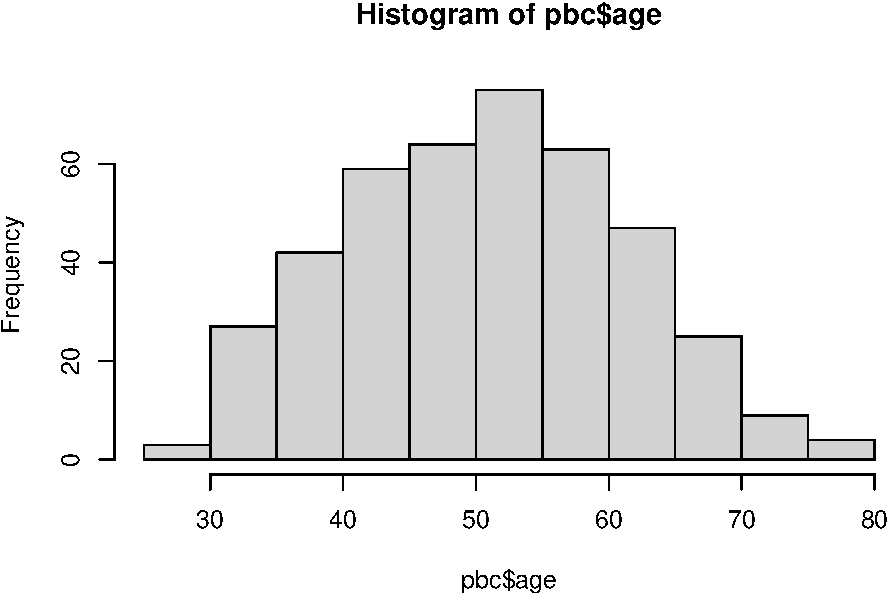
\includegraphics{phcm9795-R-notes_files/figure-latex/unnamed-chunk-28-1.pdf}

The histogram function does a remakarbly good job of choosing cutpoints and binwidths, and these rarely need to be changed. However, the labelling of the histogram should be improved by using \texttt{xlab=} and \texttt{main=} to assign labels for the x-axis and overall title respectively:

\begin{Shaded}
\begin{Highlighting}[]
\FunctionTok{hist}\NormalTok{(pbc}\SpecialCharTok{$}\NormalTok{age, }\AttributeTok{xlab=}\StringTok{"Age (years)"}\NormalTok{, }\AttributeTok{main=}\StringTok{"Histogram of participant age from pbc study data"}\NormalTok{)}
\end{Highlighting}
\end{Shaded}

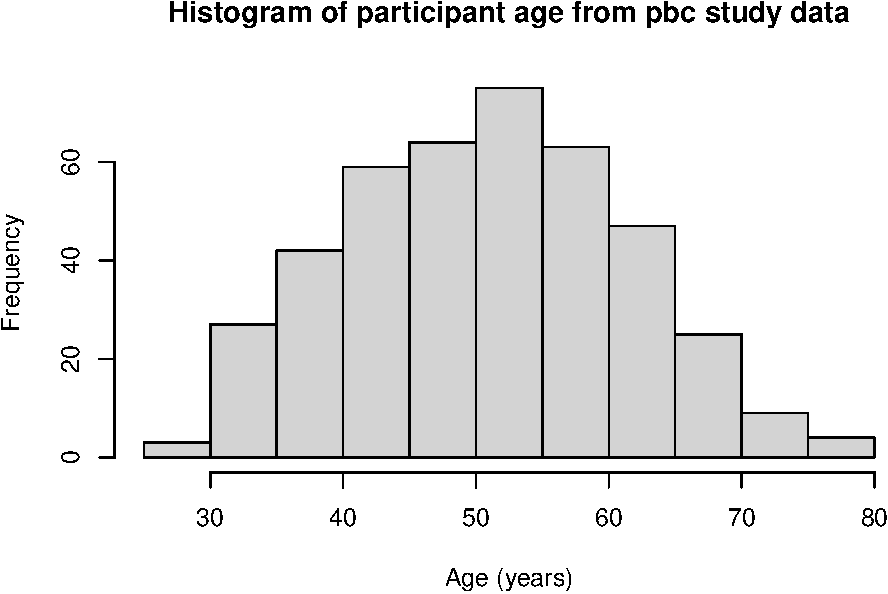
\includegraphics{phcm9795-R-notes_files/figure-latex/unnamed-chunk-29-1.pdf}

\hypertarget{producing-a-boxplot}{%
\subsection{Producing a boxplot}\label{producing-a-boxplot}}

The \texttt{boxplot} function is used to produce boxplots, again specifying the dataframe to use and the variable to be plotted as \texttt{dataframe\$variable}. Labels can be applied in the same way as the histogram:

\begin{Shaded}
\begin{Highlighting}[]
\FunctionTok{boxplot}\NormalTok{(pbc}\SpecialCharTok{$}\NormalTok{age, }\AttributeTok{xlab=}\StringTok{"Age (years)"}\NormalTok{, }\AttributeTok{main=}\StringTok{"Boxplot of participant age from pbc study data"}\NormalTok{)}
\end{Highlighting}
\end{Shaded}

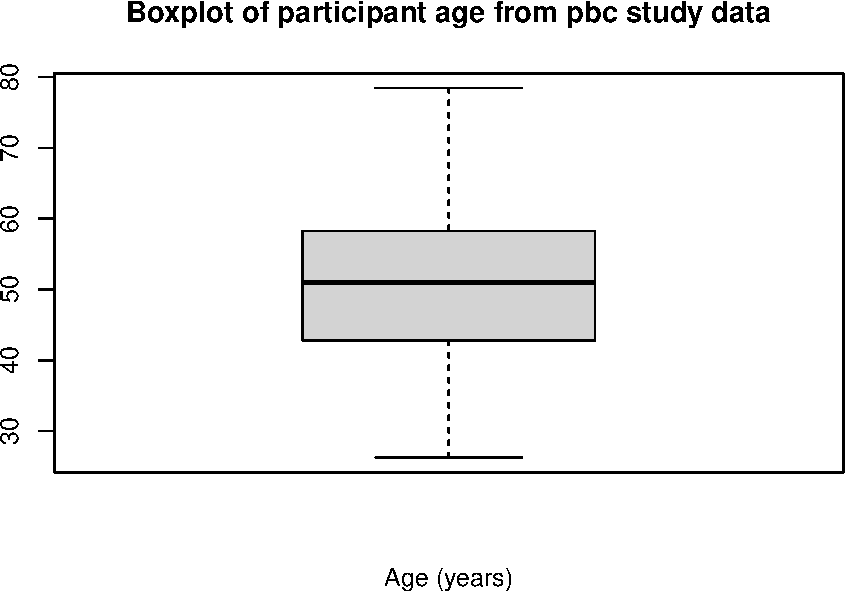
\includegraphics{phcm9795-R-notes_files/figure-latex/unnamed-chunk-30-1.pdf}

\hypertarget{producing-a-one-way-frequency-table}{%
\subsection{Producing a one-way frequency table}\label{producing-a-one-way-frequency-table}}

We have three categorical variables to summarise in Table 1: sex, stage and vital status. These variables are best summarised using one-way frequency tables.

\begin{Shaded}
\begin{Highlighting}[]
\FunctionTok{library}\NormalTok{(summarytools)}
\end{Highlighting}
\end{Shaded}

\begin{verbatim}
## 
## Attaching package: 'summarytools'
\end{verbatim}

\begin{verbatim}
## The following object is masked from 'package:tibble':
## 
##     view
\end{verbatim}

\begin{verbatim}
## The following objects are masked from 'package:huxtable':
## 
##     label, label<-
\end{verbatim}

\begin{Shaded}
\begin{Highlighting}[]
\FunctionTok{freq}\NormalTok{(pbc}\SpecialCharTok{$}\NormalTok{sex)}
\end{Highlighting}
\end{Shaded}

\begin{verbatim}
## Frequencies  
## pbc$sex  
## Type: Numeric  
## 
##               Freq   % Valid   % Valid Cum.   % Total   % Total Cum.
## ----------- ------ --------- -------------- --------- --------------
##           1     44     10.53          10.53     10.53          10.53
##           2    374     89.47         100.00     89.47         100.00
##        <NA>      0                               0.00         100.00
##       Total    418    100.00         100.00    100.00         100.00
\end{verbatim}

\hypertarget{defining-categorical-variables-as-factors}{%
\section{Defining categorical variables as factors}\label{defining-categorical-variables-as-factors}}

You will notice that the table above, in its current form, is uninterpretable as the 1 and 2 categories are not labelled. In this course, all variables including categorical variables tend to be numerically coded. To define a categorical variable as such in R, we define it as a \textbf{factor} using the \texttt{factor} function:

\texttt{factor(variable=,\ levels=,\ labels=)}

We specify:

\begin{itemize}
\tightlist
\item
  \texttt{levels}: the values the categorical variable uses can take
\item
  \texttt{labels}: the labels corresponding to each of the levels (\emph{entered in the same order as the levels})
\end{itemize}

To define our variable sex as a factor, we use:

\begin{Shaded}
\begin{Highlighting}[]
\NormalTok{pbc}\SpecialCharTok{$}\NormalTok{sex }\OtherTok{\textless{}{-}} \FunctionTok{factor}\NormalTok{(pbc}\SpecialCharTok{$}\NormalTok{sex, }\AttributeTok{levels=}\FunctionTok{c}\NormalTok{(}\DecValTok{1}\NormalTok{, }\DecValTok{2}\NormalTok{), }\AttributeTok{labels=}\FunctionTok{c}\NormalTok{(}\StringTok{"Male"}\NormalTok{, }\StringTok{"Female"}\NormalTok{))}
\end{Highlighting}
\end{Shaded}

We can confirm the coding by re-running a frequency table:

\begin{Shaded}
\begin{Highlighting}[]
\FunctionTok{freq}\NormalTok{(pbc}\SpecialCharTok{$}\NormalTok{sex)}
\end{Highlighting}
\end{Shaded}

\begin{verbatim}
## Frequencies  
## pbc$sex  
## Type: Factor  
## 
##                Freq   % Valid   % Valid Cum.   % Total   % Total Cum.
## ------------ ------ --------- -------------- --------- --------------
##         Male     44     10.53          10.53     10.53          10.53
##       Female    374     89.47         100.00     89.47         100.00
##         <NA>      0                               0.00         100.00
##        Total    418    100.00         100.00    100.00         100.00
\end{verbatim}

Task: define Stage and Vital Status as factors, and produce one-way frequency tables.

\hypertarget{copying-output-from-r-update}{%
\subsection{Copying output from R {[}UPDATE{]}}\label{copying-output-from-r-update}}

It is important to note that saving data in Stata will not save your output. Stata data and output are completely separate to one another. The easiest way to retain the output of your analyses is to copy the output into a word processor package (e.g.~Microsoft Word) before closing Stata. Once Stata is closed, all the output (that is, all your hard work!) is lost.

To copy output from Stata, you can select the output and choose Edit \textgreater{} Copy. This will copy the output as plain text for pasting into a Word document. As this is a table, you can also Copy table or Copy table as HTML. For this course, we recommend that you Copy table as HTML for pasting into Word. Whichever way you do it, you will need to make sure you reformat the table and relabel your header row and column properly for your assignments as described in Module 1. Alternatively, you can copy with the Copy table option for pasting into an Excel worksheet and reformat your table in Excel before pasting into Word.

Copying output from Stata can get a little complicated to explain. We have included a video on Moodle to summarise the different ways output can be copied.

Task: complete Table 1 using the output generated in this exercise. You should decide on whether to present continuous variables by their means or medians, and present the most appropriate measure of spread. Include footnotes to indicate if any variables contain missing observations.

\hypertarget{part-3-creating-other-types-of-graphs}{%
\section*{Part 3: Creating other types of graphs}\label{part-3-creating-other-types-of-graphs}}
\addcontentsline{toc}{section}{Part 3: Creating other types of graphs}

\hypertarget{bar-graphs}{%
\subsection{Bar graphs}\label{bar-graphs}}

Here we will create the bar chart shown in Figure 1.1 using the \texttt{pbc.dta} dataset. The x-axis of this graph will be the stage of disease, and the y-axis will show the number of participants in each category.

\hypertarget{simple-bar-graph}{%
\subsubsection{Simple bar graph}\label{simple-bar-graph}}

For most of our bar graphs, we will be plotting frequencies, so we choose \textbf{Graph of frequencies within categories}

\begin{Shaded}
\begin{Highlighting}[]
\CommentTok{\# Convert stage into a factpr}
\NormalTok{pbc}\SpecialCharTok{$}\NormalTok{stage }\OtherTok{\textless{}{-}} \FunctionTok{factor}\NormalTok{(pbc}\SpecialCharTok{$}\NormalTok{stage, }\AttributeTok{levels=}\FunctionTok{c}\NormalTok{(}\DecValTok{1}\NormalTok{,}\DecValTok{2}\NormalTok{,}\DecValTok{3}\NormalTok{,}\DecValTok{4}\NormalTok{), }\AttributeTok{labels=}\FunctionTok{c}\NormalTok{(}\StringTok{"Stage 1"}\NormalTok{, }\StringTok{"Stage 2"}\NormalTok{, }\StringTok{"Stage 3"}\NormalTok{, }\StringTok{"Stage 4"}\NormalTok{))}

\FunctionTok{plot}\NormalTok{(pbc}\SpecialCharTok{$}\NormalTok{stage, }\AttributeTok{main=}\StringTok{"Bar graph of stage of disease from PBC study"}\NormalTok{, }\AttributeTok{ylab=}\StringTok{"Number of participants"}\NormalTok{)}
\end{Highlighting}
\end{Shaded}

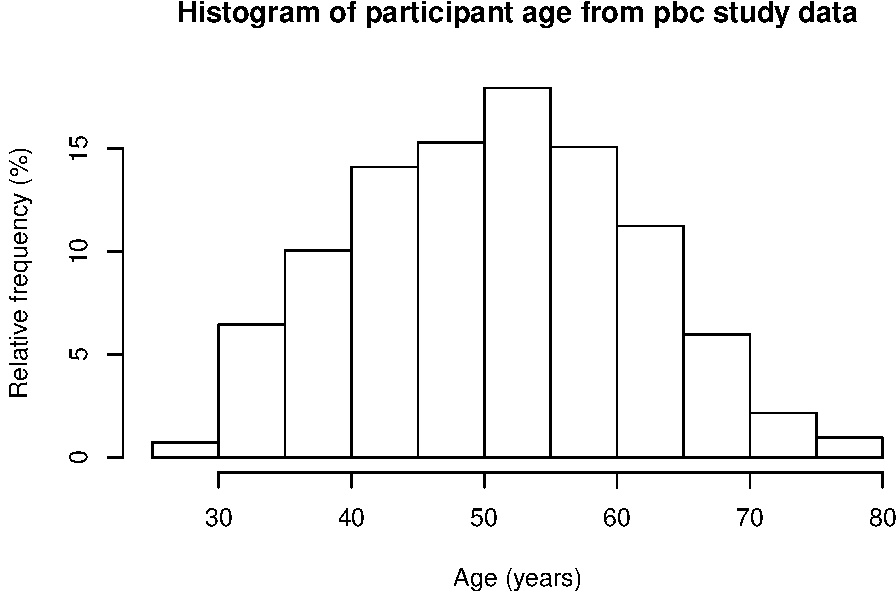
\includegraphics{phcm9795-R-notes_files/figure-latex/unnamed-chunk-34-1.pdf}

\hypertarget{clustered-bar-graph}{%
\subsection{Clustered bar graph}\label{clustered-bar-graph}}

To create a clustered bar chart as shown in Figure 1.2:

\begin{Shaded}
\begin{Highlighting}[]
\NormalTok{counts }\OtherTok{\textless{}{-}} \FunctionTok{table}\NormalTok{(pbc}\SpecialCharTok{$}\NormalTok{sex, pbc}\SpecialCharTok{$}\NormalTok{stage)}
\FunctionTok{barplot}\NormalTok{(counts, }\AttributeTok{main=}\StringTok{"Bar graph of stage of disease by sex from PBC study"}\NormalTok{,}
        \AttributeTok{legend =} \FunctionTok{rownames}\NormalTok{(counts), }\AttributeTok{beside=}\ConstantTok{TRUE}\NormalTok{, }\AttributeTok{args.legend =} \FunctionTok{list}\NormalTok{(}\AttributeTok{x =} \StringTok{"topleft"}\NormalTok{))}
\end{Highlighting}
\end{Shaded}

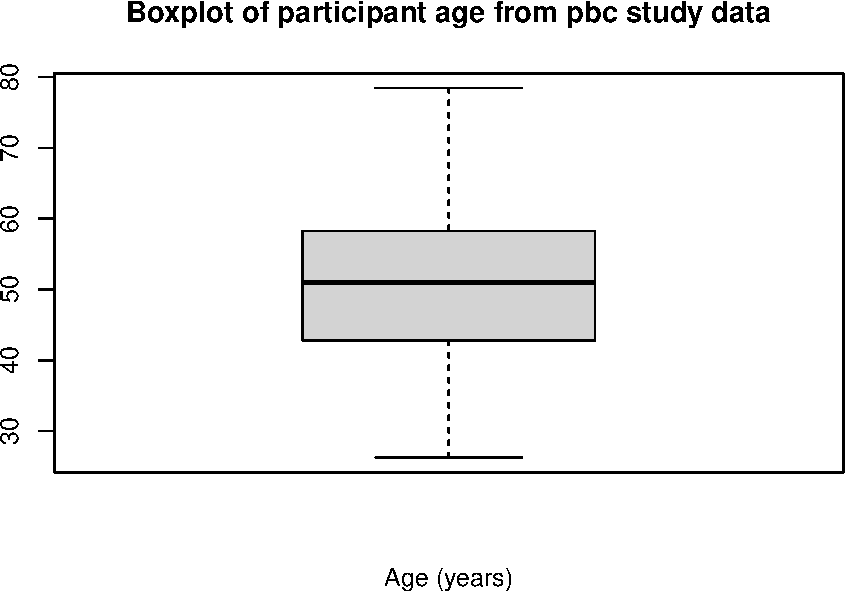
\includegraphics{phcm9795-R-notes_files/figure-latex/unnamed-chunk-35-1.pdf}

\hypertarget{stacked-bar-graph}{%
\subsection{Stacked bar graph}\label{stacked-bar-graph}}

To create a stacked bar chart shown in Figure 1.4, bring up the \textbf{Bar chart} dialog box, go to the \textbf{Options} tab and tick \textbf{Stack bars on y variables}.

\begin{Shaded}
\begin{Highlighting}[]
\FunctionTok{barplot}\NormalTok{(counts, }\AttributeTok{main=}\StringTok{"Bar graph of stage of disease by sex from PBC study"}\NormalTok{,}
        \AttributeTok{legend =} \FunctionTok{rownames}\NormalTok{(counts), }\AttributeTok{beside=}\ConstantTok{FALSE}\NormalTok{, }\AttributeTok{args.legend =} \FunctionTok{list}\NormalTok{(}\AttributeTok{x =} \StringTok{"topleft"}\NormalTok{))}
\end{Highlighting}
\end{Shaded}

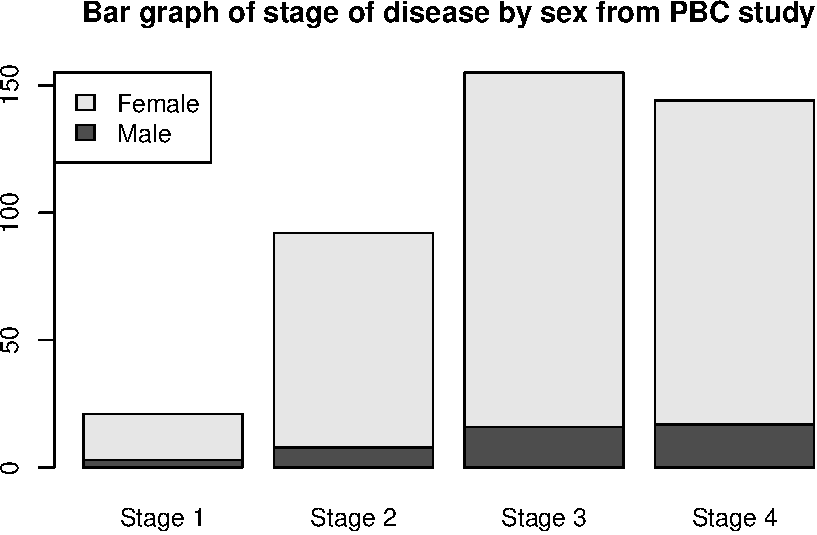
\includegraphics{phcm9795-R-notes_files/figure-latex/unnamed-chunk-36-1.pdf}

\hypertarget{stacked-bar-graph-of-relative-frequencies}{%
\subsection{Stacked bar graph of relative frequencies}\label{stacked-bar-graph-of-relative-frequencies}}

If one wants to compare the sex distribution across the stage categories, it would be convenient if all the bars have the same height (100\%). To generate such a bar chart in Stata, tick \textbf{Base bar heights on percentages} in the \textbf{Options} tab of the \textbf{Bar charts} dialog box. Change the y-axis title in the \textbf{Y axis} tab to \texttt{Percentage\ of\ students\ in\ each\ age\ group}.

\begin{Shaded}
\begin{Highlighting}[]
\NormalTok{percent }\OtherTok{\textless{}{-}} \FunctionTok{prop.table}\NormalTok{(counts, }\AttributeTok{margin=}\DecValTok{2}\NormalTok{)}\SpecialCharTok{*}\DecValTok{100}
\NormalTok{percent}
\end{Highlighting}
\end{Shaded}

\begin{verbatim}
##         
##            Stage 1   Stage 2   Stage 3   Stage 4
##   Male   14.285714  8.695652 10.322581 11.805556
##   Female 85.714286 91.304348 89.677419 88.194444
\end{verbatim}

\begin{Shaded}
\begin{Highlighting}[]
\FunctionTok{barplot}\NormalTok{(percent, }\AttributeTok{main=}\StringTok{"Relative frequency of sex within stage of disease from PBC study"}\NormalTok{,}
        \AttributeTok{legend =} \FunctionTok{rownames}\NormalTok{(counts), }\AttributeTok{beside=}\ConstantTok{FALSE}\NormalTok{, }\AttributeTok{args.legend =} \FunctionTok{list}\NormalTok{(}\AttributeTok{x =} \StringTok{"topright"}\NormalTok{))}
\end{Highlighting}
\end{Shaded}

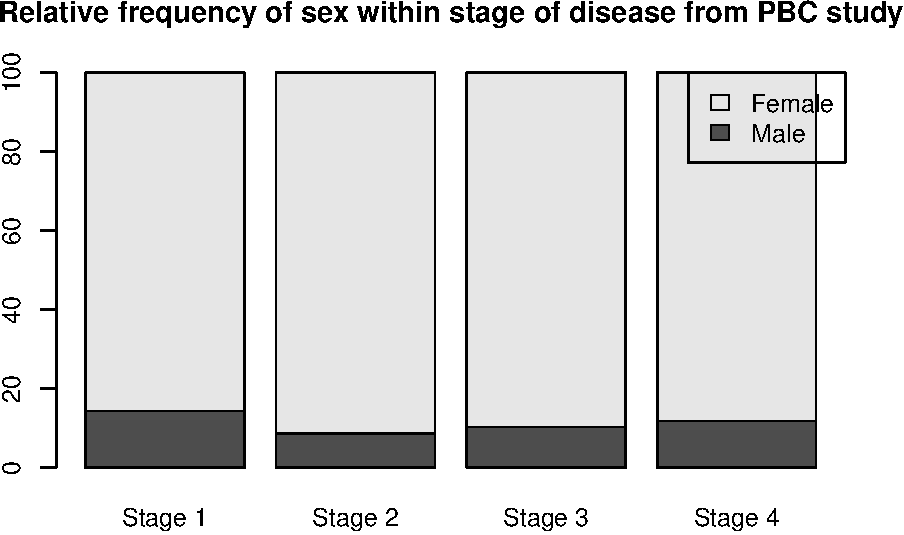
\includegraphics{phcm9795-R-notes_files/figure-latex/unnamed-chunk-37-1.pdf}

\hypertarget{creating-line-graphs}{%
\subsection{Creating line graphs}\label{creating-line-graphs}}

To demonstrate the graphing of aggregate data with Stata, we use the data on new cases and deaths from prostate cancer in males in NSW. This data has been entered into Stata as \texttt{Example\_1.2.dta}.

\begin{Shaded}
\begin{Highlighting}[]
\NormalTok{cancer }\OtherTok{\textless{}{-}} \FunctionTok{read\_stata}\NormalTok{(}\StringTok{"data/examples/Example\_1.2.dta"}\NormalTok{)}
\FunctionTok{summary}\NormalTok{(cancer)}
\end{Highlighting}
\end{Shaded}

\begin{verbatim}
##       year          ncases        ndeaths           rcases         rdeaths     
##  Min.   :1987   Min.   :1567   Min.   : 645.0   Min.   : 81.8   Min.   :31.10  
##  1st Qu.:1992   1st Qu.:2804   1st Qu.: 788.2   1st Qu.:121.9   1st Qu.:34.67  
##  Median :1996   Median :3790   Median : 868.0   Median :131.3   Median :36.55  
##  Mean   :1996   Mean   :3719   Mean   : 855.0   Mean   :135.4   Mean   :37.09  
##  3rd Qu.:2001   3rd Qu.:4403   3rd Qu.: 921.0   3rd Qu.:164.2   3rd Qu.:40.38  
##  Max.   :2006   Max.   :6158   Max.   :1044.0   Max.   :186.9   Max.   :43.80
\end{verbatim}

\begin{Shaded}
\begin{Highlighting}[]
\FunctionTok{plot}\NormalTok{(cancer}\SpecialCharTok{$}\NormalTok{year, cancer}\SpecialCharTok{$}\NormalTok{rcases, }\AttributeTok{type=}\StringTok{"l"}\NormalTok{, }\AttributeTok{col =} \StringTok{"red"}\NormalTok{, }\AttributeTok{xlab =} \StringTok{"Year"}\NormalTok{, }\AttributeTok{ylab =} \StringTok{"Age{-}standardised rate (per 100,000)"}\NormalTok{)}
\end{Highlighting}
\end{Shaded}

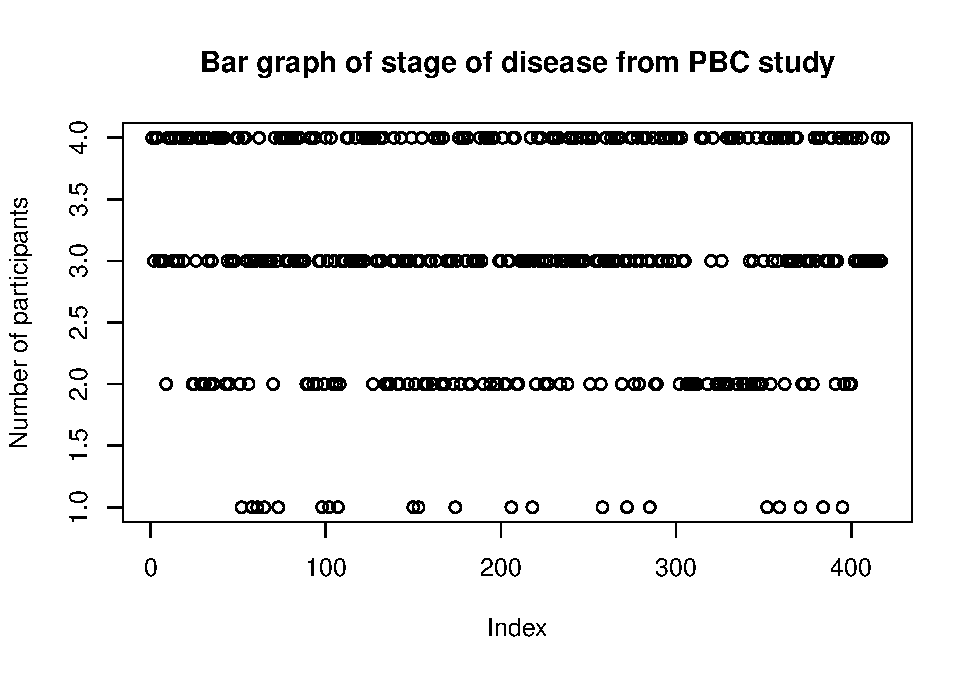
\includegraphics{phcm9795-R-notes_files/figure-latex/unnamed-chunk-38-1.pdf}

\begin{Shaded}
\begin{Highlighting}[]
\CommentTok{\# Change scale}
\FunctionTok{plot}\NormalTok{(cancer}\SpecialCharTok{$}\NormalTok{year, cancer}\SpecialCharTok{$}\NormalTok{rcases, }\AttributeTok{type=}\StringTok{"l"}\NormalTok{, }\AttributeTok{col =} \StringTok{"red"}\NormalTok{, }\AttributeTok{xlab =} \StringTok{"Year"}\NormalTok{, }\AttributeTok{ylab =} \StringTok{"Age{-}standardised rate (per 100,000)"}\NormalTok{, }\AttributeTok{ylim=}\FunctionTok{c}\NormalTok{(}\DecValTok{0}\NormalTok{,}\DecValTok{200}\NormalTok{))}

\CommentTok{\# Add a second line}
\FunctionTok{lines}\NormalTok{(cancer}\SpecialCharTok{$}\NormalTok{year, cancer}\SpecialCharTok{$}\NormalTok{rdeaths, }\AttributeTok{col =} \StringTok{"blue"}\NormalTok{, }\AttributeTok{type =} \StringTok{"l"}\NormalTok{, }\AttributeTok{lty =} \DecValTok{2}\NormalTok{)}

\CommentTok{\# Add a legend to the plot}
\FunctionTok{legend}\NormalTok{(}\StringTok{"topleft"}\NormalTok{, }\AttributeTok{legend=}\FunctionTok{c}\NormalTok{(}\StringTok{"Incidence"}\NormalTok{, }\StringTok{"Deaths"}\NormalTok{),}
       \AttributeTok{col=}\FunctionTok{c}\NormalTok{(}\StringTok{"red"}\NormalTok{, }\StringTok{"blue"}\NormalTok{), }\AttributeTok{lty =} \DecValTok{1}\SpecialCharTok{:}\DecValTok{2}\NormalTok{)}
\end{Highlighting}
\end{Shaded}

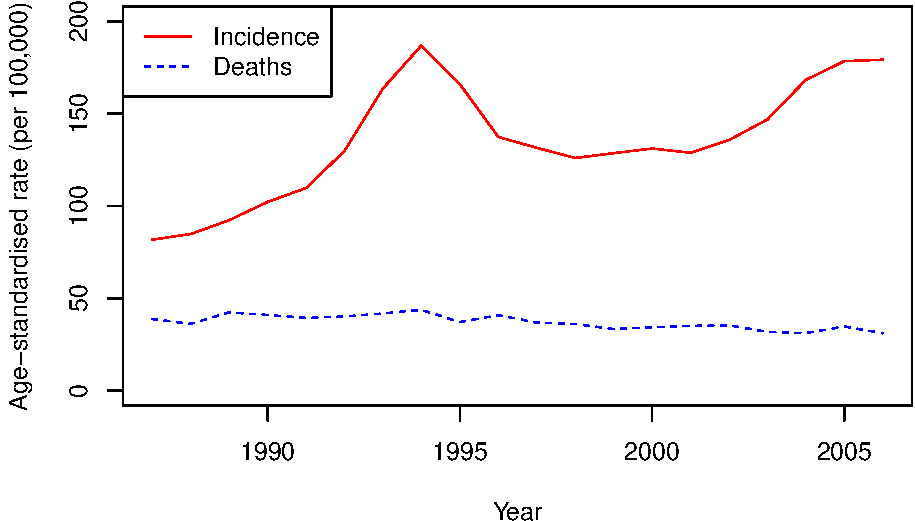
\includegraphics{phcm9795-R-notes_files/figure-latex/unnamed-chunk-38-2.pdf}

\hypertarget{probability-and-probability-distributions-r-notes}{%
\chapter{Probability and probability distributions: R notes}\label{probability-and-probability-distributions-r-notes}}

\hypertarget{importing-data-into-stata}{%
\section{Importing data into Stata}\label{importing-data-into-stata}}

We have described previously how to import data that have been saved as Stata .dta files. It is quite common to have data saved in other file types, such as Microsoft Excel, or plain text files. In this section, we will demonstrate how to import data from other packages into R.

\hypertarget{importing-plain-text-data-into-stata}{%
\subsection{Importing plain text data into Stata}\label{importing-plain-text-data-into-stata}}

A \texttt{csv} file, or a ``comma separated variables'' file is commonly used to store data. These files have a very simple structure: they are plain text files, where data are separated by commas. csv files have the advantage that, as they are plain text files, they can be opened by a large number of programs (such as Notepad in Windows, TextEdit in MacOS, Microsoft Excel - even Microsoft Word). While they can be opened by Microsoft Excel, they can be opened by many other programs: the csv file can be thought of as the lingua-franca of data.

In this demonstration, we will use data on the weight of 1000 people entered in a csv file called \texttt{weight\_s2.csv} available on Moodle.

To confirm that the file is readable by any text editor, here are the first ten lines of the file, opened in Notepad on Microsoft Windows, and TextEdit on MacOS.

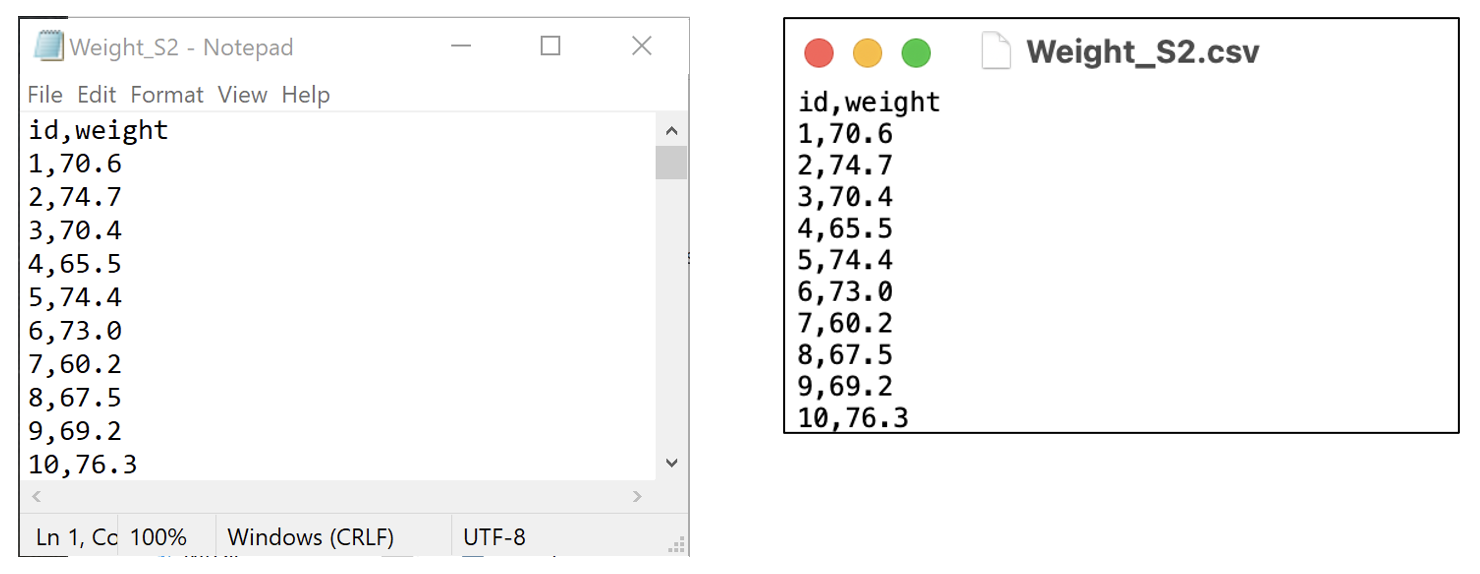
\includegraphics[width=0.66\linewidth]{img/mod02/import-01}

We can use the \texttt{read.csv} function:

\begin{Shaded}
\begin{Highlighting}[]
\FunctionTok{library}\NormalTok{(tidyverse)}
\FunctionTok{library}\NormalTok{(jmv)}

\NormalTok{weights }\OtherTok{\textless{}{-}} \FunctionTok{read.csv}\NormalTok{(}\StringTok{"data/examples/Weight\_s2.csv"}\NormalTok{)}
\end{Highlighting}
\end{Shaded}

Here, the \texttt{read.csv} function has the default that the first row of the dataset contains the variable names. If your data do not have column names, you can use \texttt{header=FALSE} in the function.

Note: there is an alternative function \texttt{read\_csv} which is part of the \texttt{readr} package (a component of the \texttt{tidyverse}). Some would argue that the \texttt{read\_csv} function is more appropriate to use because of an issue known as \texttt{strings.as.factors}. The \texttt{strings.as.factors} default was removed in R Version 4.0.0, so it is less important which of the two functions you use to import a \texttt{.csv} file. More information about this issue can be found \href{https://simplystatistics.org/posts/2015-07-24-stringsasfactors-an-unauthorized-biography}{here} and \href{https://developer.r-project.org/Blog/public/2020/02/16/stringsasfactors/}{here}.

\hypertarget{checking-your-data-for-errors-in-stata}{%
\section{Checking your data for errors in Stata}\label{checking-your-data-for-errors-in-stata}}

Before you start describing and analysing your data, it is important to make sure that no errors have been made during the data entry process. Basically, you are looking for values that are outside the range of possible or plausible values for that variable.

If an error is found, the best method for correcting the error is to go back to the original data e.g.~the hard copy questionnaire, to obtain the original value, entering the correct value into R If the original data is not available or the original data is also incorrect, the erroneous value is often excluded from the dataset.

For continuous variables, the easiest methods are to examine a boxplot and histogram. For example, a boxplot and histogram for the weight variable we just imported appear as:

\begin{Shaded}
\begin{Highlighting}[]
\FunctionTok{hist}\NormalTok{(weights}\SpecialCharTok{$}\NormalTok{weight, }\AttributeTok{xlab=}\StringTok{"Weight (kg)"}\NormalTok{, }\AttributeTok{main=}\StringTok{"Histogram of 1000 weights"}\NormalTok{)}
\end{Highlighting}
\end{Shaded}

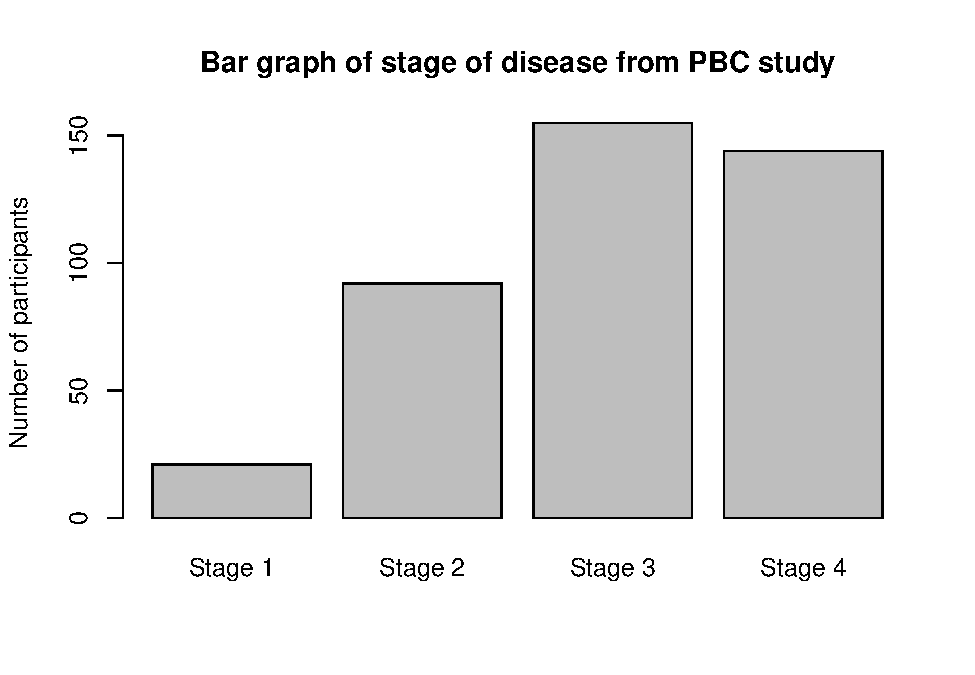
\includegraphics{phcm9795-R-notes_files/figure-latex/unnamed-chunk-41-1.pdf}

\begin{Shaded}
\begin{Highlighting}[]
\FunctionTok{boxplot}\NormalTok{(weights}\SpecialCharTok{$}\NormalTok{weight, }\AttributeTok{xlab=}\StringTok{"Weight (kg)"}\NormalTok{, }\AttributeTok{main=}\StringTok{"Boxplot of 1000 weights"}\NormalTok{)}
\end{Highlighting}
\end{Shaded}

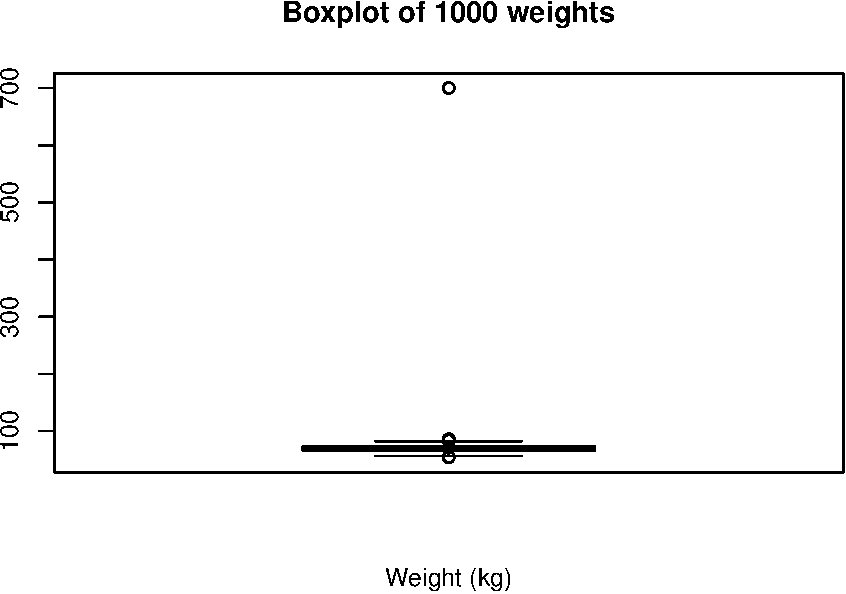
\includegraphics{phcm9795-R-notes_files/figure-latex/unnamed-chunk-41-2.pdf}

There is a clear outlying point shown in the boxplot. Although not obvious, the same point is shown in the histogram as a bar around 700 with a very short height.

We can identify any outlying observations in the dataset using the \texttt{filter} function, loaded with the \texttt{tidyverse}. You will need to decide if these values are a data entry error or are biologically plausible. If an extreme value or ``outlier'', is biologically plausible, it should be included in all analyses.

For example, to list any observations from the \texttt{weights} dataset with a weight larger than 200:

\begin{Shaded}
\begin{Highlighting}[]
\NormalTok{dplyr}\SpecialCharTok{::}\FunctionTok{filter}\NormalTok{(weights, weight}\SpecialCharTok{\textgreater{}}\DecValTok{200}\NormalTok{)}
\end{Highlighting}
\end{Shaded}

 
  \providecommand{\huxb}[2]{\arrayrulecolor[RGB]{#1}\global\arrayrulewidth=#2pt}
  \providecommand{\huxvb}[2]{\color[RGB]{#1}\vrule width #2pt}
  \providecommand{\huxtpad}[1]{\rule{0pt}{#1}}
  \providecommand{\huxbpad}[1]{\rule[-#1]{0pt}{#1}}

\begin{table}[ht]
\begin{centerbox}
\begin{threeparttable}
\captionsetup{justification=centering,singlelinecheck=off}
\caption{\label{tab:unnamed-chunk-42} }
 \setlength{\tabcolsep}{0pt}
\begin{tabular}{l l}


\hhline{>{\huxb{0, 0, 0}{0.4}}->{\huxb{0, 0, 0}{0.4}}-}
\arrayrulecolor{black}

\multicolumn{1}{!{\huxvb{0, 0, 0}{0.4}}r!{\huxvb{0, 0, 0}{0}}}{\huxtpad{6pt + 1em}\raggedleft \hspace{6pt} \textbf{id} \hspace{6pt}\huxbpad{6pt}} &
\multicolumn{1}{r!{\huxvb{0, 0, 0}{0.4}}}{\huxtpad{6pt + 1em}\raggedleft \hspace{6pt} \textbf{weight} \hspace{6pt}\huxbpad{6pt}} \tabularnewline[-0.5pt]


\hhline{>{\huxb{0, 0, 0}{0.4}}->{\huxb{0, 0, 0}{0.4}}-}
\arrayrulecolor{black}

\multicolumn{1}{!{\huxvb{0, 0, 0}{0.4}}r!{\huxvb{0, 0, 0}{0}}}{\cellcolor[RGB]{242, 242, 242}\huxtpad{6pt + 1em}\raggedleft \hspace{6pt} 58 \hspace{6pt}\huxbpad{6pt}} &
\multicolumn{1}{r!{\huxvb{0, 0, 0}{0.4}}}{\cellcolor[RGB]{242, 242, 242}\huxtpad{6pt + 1em}\raggedleft \hspace{6pt} 700 \hspace{6pt}\huxbpad{6pt}} \tabularnewline[-0.5pt]


\hhline{>{\huxb{0, 0, 0}{0.4}}->{\huxb{0, 0, 0}{0.4}}-}
\arrayrulecolor{black}
\end{tabular}
\end{threeparttable}\par\end{centerbox}

\end{table}
 

We see that there is a very high value of 700.2kg. A value as high as 700kg is likely to be a data entry error (e.g.~error in entering an extra zero) and is not a plausible weight value. Here, \textbf{you should check your original data}.

You might find that the original weight was recorded in medical records as 70.2kg. You can change this in R by writing code.

\textbf{Note:} many statistical packages, including Stata, will allow you to view a spreadsheet version of your data and edit values in that spreadsheet. This is not best practice, as corrected observations may revert to their original values depending on whether the edited data have been saved or not. By using code-based recoding, the changes will be reproduced the next time the code is run.

We will use an \texttt{ifelse} statement to recode the incorrect weight of 700.2kg into 70.2kg. The form of the \texttt{ifelse} statement is as follows:

\texttt{ifelse(test,\ value\_if\_true,\ value\_if\_false)}

Our code will create a new column (called \texttt{weight\_clean}) in the \texttt{weights} dataframe. We will test whether \texttt{weight} is equal to 700.2; if this is true, we will assign \texttt{weight\_clean} to be 70.2, otherwise \texttt{weight\_clean} will equal the value of \texttt{weight}. Putting it all together:

\begin{Shaded}
\begin{Highlighting}[]
\NormalTok{weights}\SpecialCharTok{$}\NormalTok{weight\_clean }\OtherTok{=} \FunctionTok{ifelse}\NormalTok{(weights}\SpecialCharTok{$}\NormalTok{weight}\SpecialCharTok{==}\FloatTok{700.2}\NormalTok{, }\FloatTok{70.2}\NormalTok{, weights}\SpecialCharTok{$}\NormalTok{weight)}
\end{Highlighting}
\end{Shaded}

\textbf{Note:} if an extreme value lies within the range of biological plausibility it should not be removed from analysis.

Once you have checked your data for errors, you are ready to start analysing your data.

\hypertarget{overlaying-a-normal-curve-on-a-histogram}{%
\section{Overlaying a Normal curve on a histogram}\label{overlaying-a-normal-curve-on-a-histogram}}

It can be useful to produce a histogram with an overlayed Normal curve to assess whether our sample appears approximately Normally distributed.

\hypertarget{base-graphics}{%
\subsection{Base graphics}\label{base-graphics}}

\begin{Shaded}
\begin{Highlighting}[]
\FunctionTok{hist}\NormalTok{(weights}\SpecialCharTok{$}\NormalTok{weight\_clean, }\AttributeTok{xlab=}\StringTok{"Weight (kg)"}\NormalTok{, }\AttributeTok{main=}\StringTok{"Histogram of 1000 weights"}\NormalTok{, }\AttributeTok{probability =} \ConstantTok{TRUE}\NormalTok{)}
\FunctionTok{curve}\NormalTok{(}\FunctionTok{dnorm}\NormalTok{(x, }\AttributeTok{mean=}\FunctionTok{mean}\NormalTok{(weights}\SpecialCharTok{$}\NormalTok{weight\_clean), }\AttributeTok{sd=}\FunctionTok{sd}\NormalTok{(weights}\SpecialCharTok{$}\NormalTok{weight\_clean)), }\AttributeTok{col=}\StringTok{"darkblue"}\NormalTok{, }\AttributeTok{add=}\ConstantTok{TRUE}\NormalTok{)}
\end{Highlighting}
\end{Shaded}

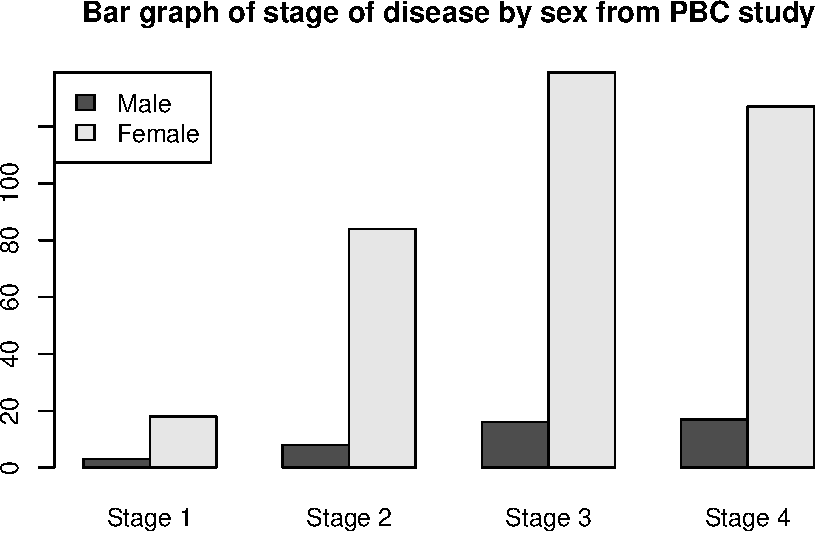
\includegraphics{phcm9795-R-notes_files/figure-latex/unnamed-chunk-44-1.pdf}

\begin{Shaded}
\begin{Highlighting}[]
\FunctionTok{hist}\NormalTok{(weights}\SpecialCharTok{$}\NormalTok{weight\_clean, }\AttributeTok{xlab=}\StringTok{"Weight (kg)"}\NormalTok{, }\AttributeTok{main=}\StringTok{"Histogram of 1000 weights"}\NormalTok{, }\AttributeTok{probability =} \ConstantTok{TRUE}\NormalTok{, }\AttributeTok{ylim=}\FunctionTok{c}\NormalTok{(}\DecValTok{0}\NormalTok{,}\FloatTok{0.1}\NormalTok{))}
\FunctionTok{curve}\NormalTok{(}\FunctionTok{dnorm}\NormalTok{(x, }\AttributeTok{mean=}\FunctionTok{mean}\NormalTok{(weights}\SpecialCharTok{$}\NormalTok{weight\_clean), }\AttributeTok{sd=}\FunctionTok{sd}\NormalTok{(weights}\SpecialCharTok{$}\NormalTok{weight\_clean)), }\AttributeTok{col=}\StringTok{"darkblue"}\NormalTok{, }\AttributeTok{add=}\ConstantTok{TRUE}\NormalTok{)}
\end{Highlighting}
\end{Shaded}

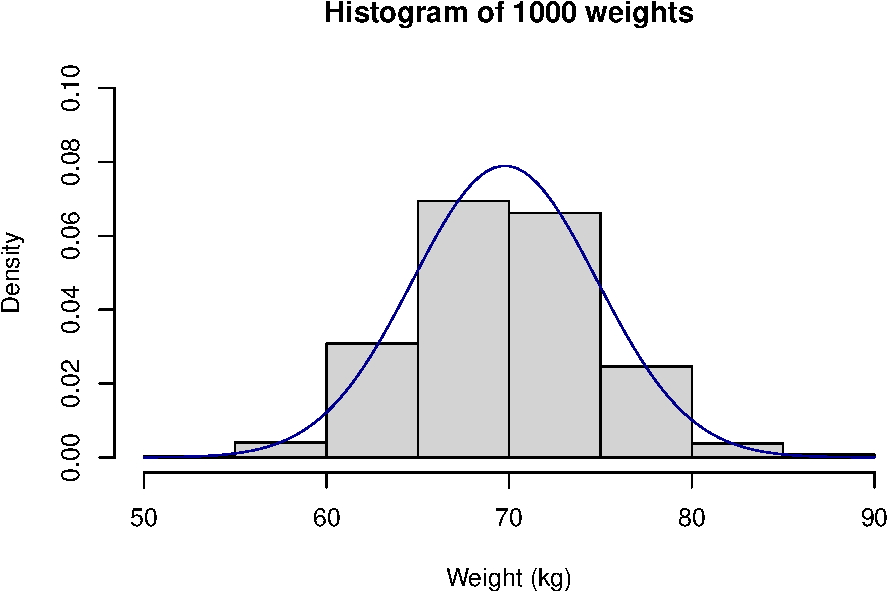
\includegraphics{phcm9795-R-notes_files/figure-latex/unnamed-chunk-44-2.pdf}

\hypertarget{ggplot2}{%
\section{ggplot2}\label{ggplot2}}

\begin{Shaded}
\begin{Highlighting}[]
\FunctionTok{ggplot}\NormalTok{(weights, }\FunctionTok{aes}\NormalTok{(}\AttributeTok{x=}\NormalTok{weight\_clean)) }\SpecialCharTok{+} \FunctionTok{geom\_histogram}\NormalTok{(}\FunctionTok{aes}\NormalTok{(}\AttributeTok{y=}\NormalTok{..density..), }\AttributeTok{breaks=}\FunctionTok{seq}\NormalTok{(}\DecValTok{50}\NormalTok{, }\DecValTok{90}\NormalTok{, }\DecValTok{5}\NormalTok{), }\AttributeTok{colour=}\StringTok{"black"}\NormalTok{, }\AttributeTok{fill=}\StringTok{"grey"}\NormalTok{) }\SpecialCharTok{+}
  \FunctionTok{stat\_function}\NormalTok{(}\AttributeTok{fun =}\NormalTok{ dnorm,}
                \AttributeTok{args =} \FunctionTok{list}\NormalTok{(}\AttributeTok{mean =} \FunctionTok{mean}\NormalTok{(weights}\SpecialCharTok{$}\NormalTok{weight\_clean),}
                            \AttributeTok{sd =} \FunctionTok{sd}\NormalTok{(weights}\SpecialCharTok{$}\NormalTok{weight\_clean)),}
                \AttributeTok{colour=}\StringTok{"darkblue"}\NormalTok{) }\SpecialCharTok{+}
  \FunctionTok{theme\_classic}\NormalTok{() }\SpecialCharTok{+}
  \FunctionTok{labs}\NormalTok{(}\AttributeTok{title=}\StringTok{"Histogram of 1000 weights"}\NormalTok{, }\AttributeTok{x=}\StringTok{"Weight (kg)"}\NormalTok{, }\AttributeTok{y=}\StringTok{"Density"}\NormalTok{)}
\end{Highlighting}
\end{Shaded}

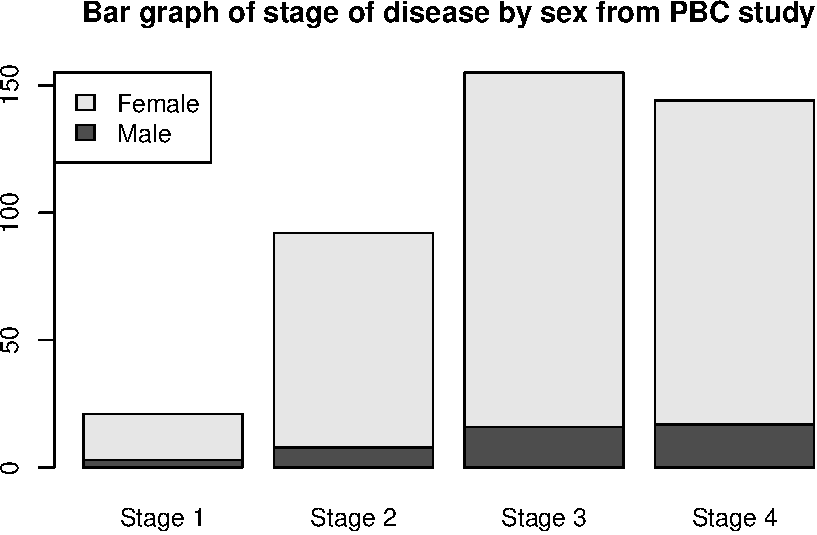
\includegraphics{phcm9795-R-notes_files/figure-latex/unnamed-chunk-45-1.pdf}

\hypertarget{descriptive-statistics-for-checking-normality}{%
\section{Descriptive statistics for checking normality}\label{descriptive-statistics-for-checking-normality}}

All the descriptive statistics including Skewness and Kurtosis discussed in this module can be obtained using the \texttt{descriptives} function from the \texttt{jmv} package. In particular, skewness and kurtosis can be requested over and above the default statistics (\texttt{skew=TRUE,\ kurt=TRUE}):

\begin{Shaded}
\begin{Highlighting}[]
\FunctionTok{descriptives}\NormalTok{(}\AttributeTok{data=}\NormalTok{weights, }\AttributeTok{vars=}\NormalTok{weight\_clean, }\AttributeTok{skew=}\ConstantTok{TRUE}\NormalTok{, }\AttributeTok{kurt=}\ConstantTok{TRUE}\NormalTok{)}
\end{Highlighting}
\end{Shaded}

\begin{verbatim}
## 
##  DESCRIPTIVES
## 
##  Descriptives                            
##  ─────────────────────────────────────── 
##                           weight_clean   
##  ─────────────────────────────────────── 
##    N                              1000   
##    Missing                           0   
##    Mean                       69.76450   
##    Median                     69.80000   
##    Standard deviation         5.052676   
##    Minimum                    53.80000   
##    Maximum                    85.80000   
##    Skewness                 0.07360659   
##    Std. error skewness      0.07734382   
##    Kurtosis                 0.05418774   
##    Std. error kurtosis       0.1545343   
##  ───────────────────────────────────────
\end{verbatim}

\hypertarget{import-excel}{%
\section{Importing Excel data into Stata}\label{import-excel}}

Another common type of file that data are stored in is a Microsoft Excel file (.xls or .xlsx). In this demonstration, we will import a selection of records from a large health survey, stored in the file \texttt{health-survey.xlsx}.

The health survey data contains 1140 records, comprising:

\begin{itemize}
\tightlist
\item
  sex: 1 = respondent identifies as male; 2 = respondent identifies as female
\item
  height: height in meters
\item
  weight: weight in kilograms
\end{itemize}

To import data from Microsoft Excel, we can use the \texttt{read\_excel()} function in the \texttt{readxl} package.

\begin{Shaded}
\begin{Highlighting}[]
\FunctionTok{library}\NormalTok{(readxl)}

\NormalTok{survey }\OtherTok{\textless{}{-}} \FunctionTok{read\_excel}\NormalTok{(}\StringTok{"data/examples/health{-}survey.xlsx"}\NormalTok{)}
\FunctionTok{summary}\NormalTok{(survey)}
\end{Highlighting}
\end{Shaded}

\begin{verbatim}
##       sex           height          weight      
##  Min.   :1.00   Min.   :1.220   Min.   : 22.70  
##  1st Qu.:1.00   1st Qu.:1.630   1st Qu.: 68.00  
##  Median :2.00   Median :1.700   Median : 79.40  
##  Mean   :1.55   Mean   :1.698   Mean   : 81.19  
##  3rd Qu.:2.00   3rd Qu.:1.780   3rd Qu.: 90.70  
##  Max.   :2.00   Max.   :2.010   Max.   :213.20
\end{verbatim}

We can see that sex has been entered as a numeric variable. We should transform it into a factor so that we can assign labels to each category:

\begin{Shaded}
\begin{Highlighting}[]
\NormalTok{survey}\SpecialCharTok{$}\NormalTok{sex }\OtherTok{\textless{}{-}} \FunctionTok{factor}\NormalTok{(survey}\SpecialCharTok{$}\NormalTok{sex, }\AttributeTok{level=}\FunctionTok{c}\NormalTok{(}\DecValTok{1}\NormalTok{,}\DecValTok{2}\NormalTok{), }\AttributeTok{labels=}\FunctionTok{c}\NormalTok{(}\StringTok{"Male"}\NormalTok{, }\StringTok{"Female"}\NormalTok{))}

\FunctionTok{summary}\NormalTok{(survey}\SpecialCharTok{$}\NormalTok{sex)}
\end{Highlighting}
\end{Shaded}

\begin{verbatim}
##   Male Female 
##    513    627
\end{verbatim}

We also note that height looks like it has been entered as meters, and weight as kilograms.

\hypertarget{generating-new-variables}{%
\section{Generating new variables}\label{generating-new-variables}}

Our health survey data contains information on height and weight. We often summarise body size using BMI: body mass index which is calculated as: \(\frac{\text{weight (kg)}}{(\text{height (m)})^2}\)

We can create a new column in our dataframe in many ways, and we will present two alternatives.

\hypertarget{base-r}{%
\subsection{Base R}\label{base-r}}

A new column can be generated using the following approach:

\texttt{dataframe\$new\_column\ =\ \textless{}formula\textgreater{}}

For example:

\begin{Shaded}
\begin{Highlighting}[]
\NormalTok{survey}\SpecialCharTok{$}\NormalTok{bmi }\OtherTok{=}\NormalTok{ survey}\SpecialCharTok{$}\NormalTok{weight }\SpecialCharTok{/}\NormalTok{ (survey}\SpecialCharTok{$}\NormalTok{height}\SpecialCharTok{\^{}}\DecValTok{2}\NormalTok{)}
\end{Highlighting}
\end{Shaded}

\hypertarget{tidyverse}{%
\subsection{tidyverse}\label{tidyverse}}

Using the tidyverse approach, we use the \texttt{mutate} command to change (or create) a column of data within the dataframe:

\begin{Shaded}
\begin{Highlighting}[]
\NormalTok{survey }\OtherTok{\textless{}{-}}\NormalTok{ survey }\SpecialCharTok{\%\textgreater{}\%} 
  \FunctionTok{mutate}\NormalTok{(}\AttributeTok{bmi =}\NormalTok{ weight }\SpecialCharTok{/}\NormalTok{ (height}\SpecialCharTok{\^{}}\DecValTok{2}\NormalTok{))}
\end{Highlighting}
\end{Shaded}

We should check the construction of the new variable by examining some records, and examining a histogram and boxplot:

\begin{Shaded}
\begin{Highlighting}[]
\FunctionTok{head}\NormalTok{(survey)}
\end{Highlighting}
\end{Shaded}

 
  \providecommand{\huxb}[2]{\arrayrulecolor[RGB]{#1}\global\arrayrulewidth=#2pt}
  \providecommand{\huxvb}[2]{\color[RGB]{#1}\vrule width #2pt}
  \providecommand{\huxtpad}[1]{\rule{0pt}{#1}}
  \providecommand{\huxbpad}[1]{\rule[-#1]{0pt}{#1}}

\begin{table}[ht]
\begin{centerbox}
\begin{threeparttable}
\captionsetup{justification=centering,singlelinecheck=off}
\caption{\label{tab:unnamed-chunk-51} }
 \setlength{\tabcolsep}{0pt}
\begin{tabular}{l l l l}


\hhline{>{\huxb{0, 0, 0}{0.4}}->{\huxb{0, 0, 0}{0.4}}->{\huxb{0, 0, 0}{0.4}}->{\huxb{0, 0, 0}{0.4}}-}
\arrayrulecolor{black}

\multicolumn{1}{!{\huxvb{0, 0, 0}{0.4}}l!{\huxvb{0, 0, 0}{0}}}{\huxtpad{6pt + 1em}\raggedright \hspace{6pt} \textbf{sex} \hspace{6pt}\huxbpad{6pt}} &
\multicolumn{1}{r!{\huxvb{0, 0, 0}{0}}}{\huxtpad{6pt + 1em}\raggedleft \hspace{6pt} \textbf{height} \hspace{6pt}\huxbpad{6pt}} &
\multicolumn{1}{r!{\huxvb{0, 0, 0}{0}}}{\huxtpad{6pt + 1em}\raggedleft \hspace{6pt} \textbf{weight} \hspace{6pt}\huxbpad{6pt}} &
\multicolumn{1}{r!{\huxvb{0, 0, 0}{0.4}}}{\huxtpad{6pt + 1em}\raggedleft \hspace{6pt} \textbf{bmi} \hspace{6pt}\huxbpad{6pt}} \tabularnewline[-0.5pt]


\hhline{>{\huxb{0, 0, 0}{0.4}}->{\huxb{0, 0, 0}{0.4}}->{\huxb{0, 0, 0}{0.4}}->{\huxb{0, 0, 0}{0.4}}-}
\arrayrulecolor{black}

\multicolumn{1}{!{\huxvb{0, 0, 0}{0.4}}l!{\huxvb{0, 0, 0}{0}}}{\cellcolor[RGB]{242, 242, 242}\huxtpad{6pt + 1em}\raggedright \hspace{6pt} Male \hspace{6pt}\huxbpad{6pt}} &
\multicolumn{1}{r!{\huxvb{0, 0, 0}{0}}}{\cellcolor[RGB]{242, 242, 242}\huxtpad{6pt + 1em}\raggedleft \hspace{6pt} 1.63 \hspace{6pt}\huxbpad{6pt}} &
\multicolumn{1}{r!{\huxvb{0, 0, 0}{0}}}{\cellcolor[RGB]{242, 242, 242}\huxtpad{6pt + 1em}\raggedleft \hspace{6pt} 81.7 \hspace{6pt}\huxbpad{6pt}} &
\multicolumn{1}{r!{\huxvb{0, 0, 0}{0.4}}}{\cellcolor[RGB]{242, 242, 242}\huxtpad{6pt + 1em}\raggedleft \hspace{6pt} 30.8 \hspace{6pt}\huxbpad{6pt}} \tabularnewline[-0.5pt]


\hhline{>{\huxb{0, 0, 0}{0.4}}|>{\huxb{0, 0, 0}{0.4}}|}
\arrayrulecolor{black}

\multicolumn{1}{!{\huxvb{0, 0, 0}{0.4}}l!{\huxvb{0, 0, 0}{0}}}{\huxtpad{6pt + 1em}\raggedright \hspace{6pt} Male \hspace{6pt}\huxbpad{6pt}} &
\multicolumn{1}{r!{\huxvb{0, 0, 0}{0}}}{\huxtpad{6pt + 1em}\raggedleft \hspace{6pt} 1.63 \hspace{6pt}\huxbpad{6pt}} &
\multicolumn{1}{r!{\huxvb{0, 0, 0}{0}}}{\huxtpad{6pt + 1em}\raggedleft \hspace{6pt} 68\hphantom{0}\hphantom{0} \hspace{6pt}\huxbpad{6pt}} &
\multicolumn{1}{r!{\huxvb{0, 0, 0}{0.4}}}{\huxtpad{6pt + 1em}\raggedleft \hspace{6pt} 25.6 \hspace{6pt}\huxbpad{6pt}} \tabularnewline[-0.5pt]


\hhline{>{\huxb{0, 0, 0}{0.4}}|>{\huxb{0, 0, 0}{0.4}}|}
\arrayrulecolor{black}

\multicolumn{1}{!{\huxvb{0, 0, 0}{0.4}}l!{\huxvb{0, 0, 0}{0}}}{\cellcolor[RGB]{242, 242, 242}\huxtpad{6pt + 1em}\raggedright \hspace{6pt} Male \hspace{6pt}\huxbpad{6pt}} &
\multicolumn{1}{r!{\huxvb{0, 0, 0}{0}}}{\cellcolor[RGB]{242, 242, 242}\huxtpad{6pt + 1em}\raggedleft \hspace{6pt} 1.85 \hspace{6pt}\huxbpad{6pt}} &
\multicolumn{1}{r!{\huxvb{0, 0, 0}{0}}}{\cellcolor[RGB]{242, 242, 242}\huxtpad{6pt + 1em}\raggedleft \hspace{6pt} 97.1 \hspace{6pt}\huxbpad{6pt}} &
\multicolumn{1}{r!{\huxvb{0, 0, 0}{0.4}}}{\cellcolor[RGB]{242, 242, 242}\huxtpad{6pt + 1em}\raggedleft \hspace{6pt} 28.4 \hspace{6pt}\huxbpad{6pt}} \tabularnewline[-0.5pt]


\hhline{>{\huxb{0, 0, 0}{0.4}}|>{\huxb{0, 0, 0}{0.4}}|}
\arrayrulecolor{black}

\multicolumn{1}{!{\huxvb{0, 0, 0}{0.4}}l!{\huxvb{0, 0, 0}{0}}}{\huxtpad{6pt + 1em}\raggedright \hspace{6pt} Male \hspace{6pt}\huxbpad{6pt}} &
\multicolumn{1}{r!{\huxvb{0, 0, 0}{0}}}{\huxtpad{6pt + 1em}\raggedleft \hspace{6pt} 1.78 \hspace{6pt}\huxbpad{6pt}} &
\multicolumn{1}{r!{\huxvb{0, 0, 0}{0}}}{\huxtpad{6pt + 1em}\raggedleft \hspace{6pt} 89.8 \hspace{6pt}\huxbpad{6pt}} &
\multicolumn{1}{r!{\huxvb{0, 0, 0}{0.4}}}{\huxtpad{6pt + 1em}\raggedleft \hspace{6pt} 28.3 \hspace{6pt}\huxbpad{6pt}} \tabularnewline[-0.5pt]


\hhline{>{\huxb{0, 0, 0}{0.4}}|>{\huxb{0, 0, 0}{0.4}}|}
\arrayrulecolor{black}

\multicolumn{1}{!{\huxvb{0, 0, 0}{0.4}}l!{\huxvb{0, 0, 0}{0}}}{\cellcolor[RGB]{242, 242, 242}\huxtpad{6pt + 1em}\raggedright \hspace{6pt} Male \hspace{6pt}\huxbpad{6pt}} &
\multicolumn{1}{r!{\huxvb{0, 0, 0}{0}}}{\cellcolor[RGB]{242, 242, 242}\huxtpad{6pt + 1em}\raggedleft \hspace{6pt} 1.73 \hspace{6pt}\huxbpad{6pt}} &
\multicolumn{1}{r!{\huxvb{0, 0, 0}{0}}}{\cellcolor[RGB]{242, 242, 242}\huxtpad{6pt + 1em}\raggedleft \hspace{6pt} 70.3 \hspace{6pt}\huxbpad{6pt}} &
\multicolumn{1}{r!{\huxvb{0, 0, 0}{0.4}}}{\cellcolor[RGB]{242, 242, 242}\huxtpad{6pt + 1em}\raggedleft \hspace{6pt} 23.5 \hspace{6pt}\huxbpad{6pt}} \tabularnewline[-0.5pt]


\hhline{>{\huxb{0, 0, 0}{0.4}}|>{\huxb{0, 0, 0}{0.4}}|}
\arrayrulecolor{black}

\multicolumn{1}{!{\huxvb{0, 0, 0}{0.4}}l!{\huxvb{0, 0, 0}{0}}}{\huxtpad{6pt + 1em}\raggedright \hspace{6pt} Female \hspace{6pt}\huxbpad{6pt}} &
\multicolumn{1}{r!{\huxvb{0, 0, 0}{0}}}{\huxtpad{6pt + 1em}\raggedleft \hspace{6pt} 1.57 \hspace{6pt}\huxbpad{6pt}} &
\multicolumn{1}{r!{\huxvb{0, 0, 0}{0}}}{\huxtpad{6pt + 1em}\raggedleft \hspace{6pt} 85.7 \hspace{6pt}\huxbpad{6pt}} &
\multicolumn{1}{r!{\huxvb{0, 0, 0}{0.4}}}{\huxtpad{6pt + 1em}\raggedleft \hspace{6pt} 34.8 \hspace{6pt}\huxbpad{6pt}} \tabularnewline[-0.5pt]


\hhline{>{\huxb{0, 0, 0}{0.4}}->{\huxb{0, 0, 0}{0.4}}->{\huxb{0, 0, 0}{0.4}}->{\huxb{0, 0, 0}{0.4}}-}
\arrayrulecolor{black}
\end{tabular}
\end{threeparttable}\par\end{centerbox}

\end{table}
 

\begin{Shaded}
\begin{Highlighting}[]
\FunctionTok{tail}\NormalTok{(survey)}
\end{Highlighting}
\end{Shaded}

 
  \providecommand{\huxb}[2]{\arrayrulecolor[RGB]{#1}\global\arrayrulewidth=#2pt}
  \providecommand{\huxvb}[2]{\color[RGB]{#1}\vrule width #2pt}
  \providecommand{\huxtpad}[1]{\rule{0pt}{#1}}
  \providecommand{\huxbpad}[1]{\rule[-#1]{0pt}{#1}}

\begin{table}[ht]
\begin{centerbox}
\begin{threeparttable}
\captionsetup{justification=centering,singlelinecheck=off}
\caption{\label{tab:unnamed-chunk-51} }
 \setlength{\tabcolsep}{0pt}
\begin{tabular}{l l l l}


\hhline{>{\huxb{0, 0, 0}{0.4}}->{\huxb{0, 0, 0}{0.4}}->{\huxb{0, 0, 0}{0.4}}->{\huxb{0, 0, 0}{0.4}}-}
\arrayrulecolor{black}

\multicolumn{1}{!{\huxvb{0, 0, 0}{0.4}}l!{\huxvb{0, 0, 0}{0}}}{\huxtpad{6pt + 1em}\raggedright \hspace{6pt} \textbf{sex} \hspace{6pt}\huxbpad{6pt}} &
\multicolumn{1}{r!{\huxvb{0, 0, 0}{0}}}{\huxtpad{6pt + 1em}\raggedleft \hspace{6pt} \textbf{height} \hspace{6pt}\huxbpad{6pt}} &
\multicolumn{1}{r!{\huxvb{0, 0, 0}{0}}}{\huxtpad{6pt + 1em}\raggedleft \hspace{6pt} \textbf{weight} \hspace{6pt}\huxbpad{6pt}} &
\multicolumn{1}{r!{\huxvb{0, 0, 0}{0.4}}}{\huxtpad{6pt + 1em}\raggedleft \hspace{6pt} \textbf{bmi} \hspace{6pt}\huxbpad{6pt}} \tabularnewline[-0.5pt]


\hhline{>{\huxb{0, 0, 0}{0.4}}->{\huxb{0, 0, 0}{0.4}}->{\huxb{0, 0, 0}{0.4}}->{\huxb{0, 0, 0}{0.4}}-}
\arrayrulecolor{black}

\multicolumn{1}{!{\huxvb{0, 0, 0}{0.4}}l!{\huxvb{0, 0, 0}{0}}}{\cellcolor[RGB]{242, 242, 242}\huxtpad{6pt + 1em}\raggedright \hspace{6pt} Female \hspace{6pt}\huxbpad{6pt}} &
\multicolumn{1}{r!{\huxvb{0, 0, 0}{0}}}{\cellcolor[RGB]{242, 242, 242}\huxtpad{6pt + 1em}\raggedleft \hspace{6pt} 1.65 \hspace{6pt}\huxbpad{6pt}} &
\multicolumn{1}{r!{\huxvb{0, 0, 0}{0}}}{\cellcolor[RGB]{242, 242, 242}\huxtpad{6pt + 1em}\raggedleft \hspace{6pt} 95.7 \hspace{6pt}\huxbpad{6pt}} &
\multicolumn{1}{r!{\huxvb{0, 0, 0}{0.4}}}{\cellcolor[RGB]{242, 242, 242}\huxtpad{6pt + 1em}\raggedleft \hspace{6pt} 35.2 \hspace{6pt}\huxbpad{6pt}} \tabularnewline[-0.5pt]


\hhline{>{\huxb{0, 0, 0}{0.4}}|>{\huxb{0, 0, 0}{0.4}}|}
\arrayrulecolor{black}

\multicolumn{1}{!{\huxvb{0, 0, 0}{0.4}}l!{\huxvb{0, 0, 0}{0}}}{\huxtpad{6pt + 1em}\raggedright \hspace{6pt} Male \hspace{6pt}\huxbpad{6pt}} &
\multicolumn{1}{r!{\huxvb{0, 0, 0}{0}}}{\huxtpad{6pt + 1em}\raggedleft \hspace{6pt} 1.8\hphantom{0} \hspace{6pt}\huxbpad{6pt}} &
\multicolumn{1}{r!{\huxvb{0, 0, 0}{0}}}{\huxtpad{6pt + 1em}\raggedleft \hspace{6pt} 79.4 \hspace{6pt}\huxbpad{6pt}} &
\multicolumn{1}{r!{\huxvb{0, 0, 0}{0.4}}}{\huxtpad{6pt + 1em}\raggedleft \hspace{6pt} 24.5 \hspace{6pt}\huxbpad{6pt}} \tabularnewline[-0.5pt]


\hhline{>{\huxb{0, 0, 0}{0.4}}|>{\huxb{0, 0, 0}{0.4}}|}
\arrayrulecolor{black}

\multicolumn{1}{!{\huxvb{0, 0, 0}{0.4}}l!{\huxvb{0, 0, 0}{0}}}{\cellcolor[RGB]{242, 242, 242}\huxtpad{6pt + 1em}\raggedright \hspace{6pt} Female \hspace{6pt}\huxbpad{6pt}} &
\multicolumn{1}{r!{\huxvb{0, 0, 0}{0}}}{\cellcolor[RGB]{242, 242, 242}\huxtpad{6pt + 1em}\raggedleft \hspace{6pt} 1.73 \hspace{6pt}\huxbpad{6pt}} &
\multicolumn{1}{r!{\huxvb{0, 0, 0}{0}}}{\cellcolor[RGB]{242, 242, 242}\huxtpad{6pt + 1em}\raggedleft \hspace{6pt} 83\hphantom{0}\hphantom{0} \hspace{6pt}\huxbpad{6pt}} &
\multicolumn{1}{r!{\huxvb{0, 0, 0}{0.4}}}{\cellcolor[RGB]{242, 242, 242}\huxtpad{6pt + 1em}\raggedleft \hspace{6pt} 27.7 \hspace{6pt}\huxbpad{6pt}} \tabularnewline[-0.5pt]


\hhline{>{\huxb{0, 0, 0}{0.4}}|>{\huxb{0, 0, 0}{0.4}}|}
\arrayrulecolor{black}

\multicolumn{1}{!{\huxvb{0, 0, 0}{0.4}}l!{\huxvb{0, 0, 0}{0}}}{\huxtpad{6pt + 1em}\raggedright \hspace{6pt} Female \hspace{6pt}\huxbpad{6pt}} &
\multicolumn{1}{r!{\huxvb{0, 0, 0}{0}}}{\huxtpad{6pt + 1em}\raggedleft \hspace{6pt} 1.57 \hspace{6pt}\huxbpad{6pt}} &
\multicolumn{1}{r!{\huxvb{0, 0, 0}{0}}}{\huxtpad{6pt + 1em}\raggedleft \hspace{6pt} 61.2 \hspace{6pt}\huxbpad{6pt}} &
\multicolumn{1}{r!{\huxvb{0, 0, 0}{0.4}}}{\huxtpad{6pt + 1em}\raggedleft \hspace{6pt} 24.8 \hspace{6pt}\huxbpad{6pt}} \tabularnewline[-0.5pt]


\hhline{>{\huxb{0, 0, 0}{0.4}}|>{\huxb{0, 0, 0}{0.4}}|}
\arrayrulecolor{black}

\multicolumn{1}{!{\huxvb{0, 0, 0}{0.4}}l!{\huxvb{0, 0, 0}{0}}}{\cellcolor[RGB]{242, 242, 242}\huxtpad{6pt + 1em}\raggedright \hspace{6pt} Male \hspace{6pt}\huxbpad{6pt}} &
\multicolumn{1}{r!{\huxvb{0, 0, 0}{0}}}{\cellcolor[RGB]{242, 242, 242}\huxtpad{6pt + 1em}\raggedleft \hspace{6pt} 1.7\hphantom{0} \hspace{6pt}\huxbpad{6pt}} &
\multicolumn{1}{r!{\huxvb{0, 0, 0}{0}}}{\cellcolor[RGB]{242, 242, 242}\huxtpad{6pt + 1em}\raggedleft \hspace{6pt} 73\hphantom{0}\hphantom{0} \hspace{6pt}\huxbpad{6pt}} &
\multicolumn{1}{r!{\huxvb{0, 0, 0}{0.4}}}{\cellcolor[RGB]{242, 242, 242}\huxtpad{6pt + 1em}\raggedleft \hspace{6pt} 25.3 \hspace{6pt}\huxbpad{6pt}} \tabularnewline[-0.5pt]


\hhline{>{\huxb{0, 0, 0}{0.4}}|>{\huxb{0, 0, 0}{0.4}}|}
\arrayrulecolor{black}

\multicolumn{1}{!{\huxvb{0, 0, 0}{0.4}}l!{\huxvb{0, 0, 0}{0}}}{\huxtpad{6pt + 1em}\raggedright \hspace{6pt} Female \hspace{6pt}\huxbpad{6pt}} &
\multicolumn{1}{r!{\huxvb{0, 0, 0}{0}}}{\huxtpad{6pt + 1em}\raggedleft \hspace{6pt} 1.55 \hspace{6pt}\huxbpad{6pt}} &
\multicolumn{1}{r!{\huxvb{0, 0, 0}{0}}}{\huxtpad{6pt + 1em}\raggedleft \hspace{6pt} 91.2 \hspace{6pt}\huxbpad{6pt}} &
\multicolumn{1}{r!{\huxvb{0, 0, 0}{0.4}}}{\huxtpad{6pt + 1em}\raggedleft \hspace{6pt} 38\hphantom{0}\hphantom{0} \hspace{6pt}\huxbpad{6pt}} \tabularnewline[-0.5pt]


\hhline{>{\huxb{0, 0, 0}{0.4}}->{\huxb{0, 0, 0}{0.4}}->{\huxb{0, 0, 0}{0.4}}->{\huxb{0, 0, 0}{0.4}}-}
\arrayrulecolor{black}
\end{tabular}
\end{threeparttable}\par\end{centerbox}

\end{table}
 

\begin{Shaded}
\begin{Highlighting}[]
\FunctionTok{hist}\NormalTok{(survey}\SpecialCharTok{$}\NormalTok{bmi)}
\end{Highlighting}
\end{Shaded}

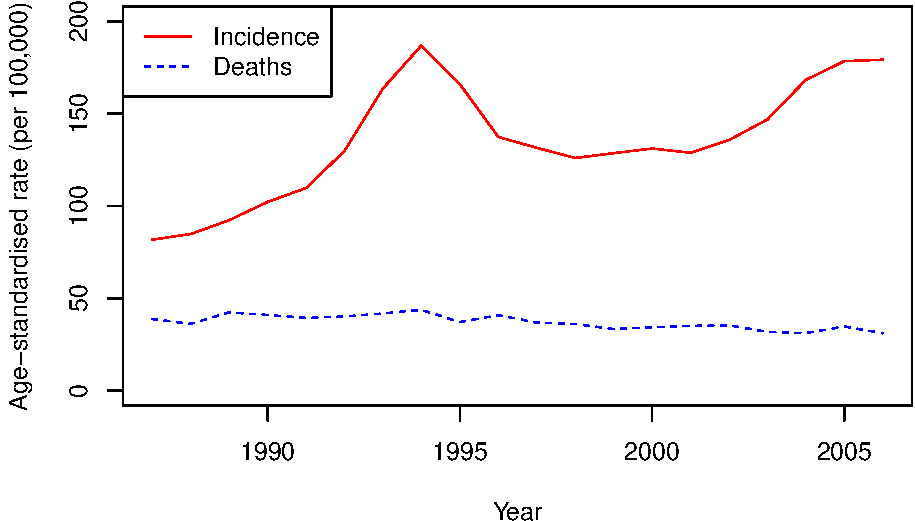
\includegraphics{phcm9795-R-notes_files/figure-latex/unnamed-chunk-51-1.pdf}

\begin{Shaded}
\begin{Highlighting}[]
\FunctionTok{boxplot}\NormalTok{(survey}\SpecialCharTok{$}\NormalTok{bmi)}
\end{Highlighting}
\end{Shaded}

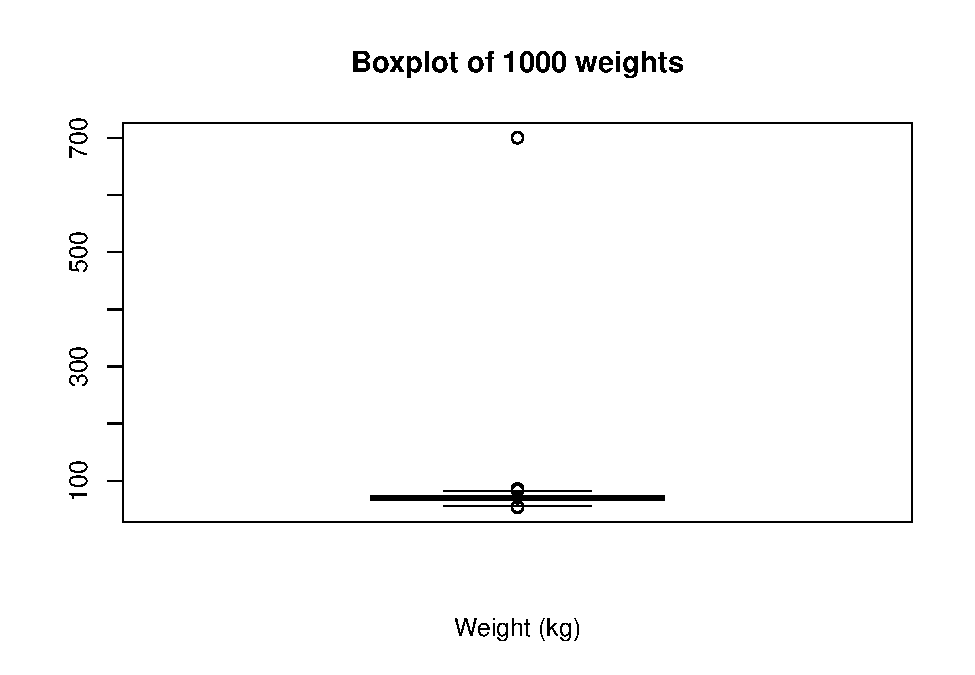
\includegraphics{phcm9795-R-notes_files/figure-latex/unnamed-chunk-51-2.pdf}

In the general population, BMI ranges between about 15 to 30. It appears that BMI has been correctly generated in this example. We should investigate the very low and some of the very high values of BMI, but this will be left for another time.

\hypertarget{summarising-data-by-another-variable}{%
\section{Summarising data by another variable}\label{summarising-data-by-another-variable}}

We will often want to calculate the same summary statistics by another variable. For example, we might want to calculate summary statistics for BMI for males and females separately. We can do this in in the \texttt{descriptives} function by defining sex as a \texttt{splitBy} variable:

\begin{Shaded}
\begin{Highlighting}[]
\FunctionTok{descriptives}\NormalTok{(}\AttributeTok{data=}\NormalTok{survey, }\AttributeTok{vars=}\NormalTok{bmi, }\AttributeTok{splitBy =}\NormalTok{ sex)}
\end{Highlighting}
\end{Shaded}

\begin{verbatim}
## 
##  DESCRIPTIVES
## 
##  Descriptives                                 
##  ──────────────────────────────────────────── 
##                          sex       bmi        
##  ──────────────────────────────────────────── 
##    N                     Male           513   
##                          Female         627   
##    Missing               Male             0   
##                          Female           0   
##    Mean                  Male      28.29561   
##                          Female    27.81434   
##    Median                Male      27.39592   
##                          Female    26.66667   
##    Standard deviation    Male      5.204975   
##                          Female    6.380523   
##    Minimum               Male      16.47519   
##                          Female    9.209299   
##    Maximum               Male      57.23644   
##                          Female    52.59516   
##  ────────────────────────────────────────────
\end{verbatim}

{[}PLOTS BY VARIABLES{]}

\hypertarget{recoding-data}{%
\section{Recoding data}\label{recoding-data}}

One task that is common in statistical computing is to recode variables. For example, we might want to group some categories of a categorical variable, or to present a continuous variable in a categorical way.

In this example, we can recode BMI into the following categories as suggested by the World Health Organisation {[}footnote{]}:

\begin{itemize}
\tightlist
\item
  Underweight: BMI \textless{} 18.5
\item
  Normal weight: 18.5 \(\le\) BMI \textless{} 25
\item
  Pre-obesity: 25 \(\le\) BMI \textless{} 30
\item
  Obesity Class I: 30 \(\le\) BMI \textless{} 35
\item
  Obesity Class II: 35 \(\le\) BMI \textless{} 40
\item
  Obesity Class III: BMI \(\ge\) 40
\end{itemize}

The quickest way to recode a continuous variable into categories is to use the \texttt{cut} command which takes a continuous variable, and ``cuts'' it into groups based on the specified ``cutpoints'':

\begin{Shaded}
\begin{Highlighting}[]
\NormalTok{survey}\SpecialCharTok{$}\NormalTok{bmi\_cat }\OtherTok{\textless{}{-}} \FunctionTok{cut}\NormalTok{(survey}\SpecialCharTok{$}\NormalTok{bmi, }\FunctionTok{c}\NormalTok{(}\DecValTok{0}\NormalTok{, }\FloatTok{18.5}\NormalTok{, }\DecValTok{25}\NormalTok{, }\DecValTok{30}\NormalTok{, }\DecValTok{35}\NormalTok{, }\DecValTok{40}\NormalTok{, }\DecValTok{100}\NormalTok{))}
\end{Highlighting}
\end{Shaded}

Notice that lower (BMI=0) and upper (BMI=100) bounds have been specified, as both a lower and upper limit must be defined for each group.

If we examine the new \texttt{bmi\_cat} variable:

\begin{Shaded}
\begin{Highlighting}[]
\FunctionTok{summary}\NormalTok{(survey}\SpecialCharTok{$}\NormalTok{bmi\_cat)}
\end{Highlighting}
\end{Shaded}

\begin{verbatim}
##  (0,18.5] (18.5,25]   (25,30]   (30,35]   (35,40]  (40,100] 
##        18       362       411       205        97        47
\end{verbatim}

we see that each group has been labelled (a, b{]}. This notation is equivalent to: greater than a, and less than or equal to b. The \texttt{cut} function excludes the lower limit, but includes the upper limit. Our BMI ranges have been defined to include the lower limit, and exclude the upper limit (for example, greater than or equal to 30 and less than 35).

We can specify this recoding using the \texttt{right=FALSE} option:

\begin{Shaded}
\begin{Highlighting}[]
\NormalTok{survey}\SpecialCharTok{$}\NormalTok{bmi\_cat }\OtherTok{\textless{}{-}} \FunctionTok{cut}\NormalTok{(survey}\SpecialCharTok{$}\NormalTok{bmi, }\FunctionTok{c}\NormalTok{(}\DecValTok{0}\NormalTok{, }\FloatTok{18.5}\NormalTok{, }\DecValTok{25}\NormalTok{, }\DecValTok{30}\NormalTok{, }\DecValTok{35}\NormalTok{, }\DecValTok{40}\NormalTok{, }\DecValTok{100}\NormalTok{), }\AttributeTok{right=}\ConstantTok{FALSE}\NormalTok{)}
\FunctionTok{summary}\NormalTok{(survey}\SpecialCharTok{$}\NormalTok{bmi\_cat)}
\end{Highlighting}
\end{Shaded}

\begin{verbatim}
##  [0,18.5) [18.5,25)   [25,30)   [30,35)   [35,40)  [40,100) 
##        18       362       411       201       101        47
\end{verbatim}

More complex recoding can be done using the \texttt{case\_when} command in the \texttt{dplyr} package.

{[}INCLUDE???{]}

\hypertarget{computing-binomial-probabilities-using-r}{%
\section{Computing binomial probabilities using R}\label{computing-binomial-probabilities-using-r}}

There are two R functions that we can use to calculate probabilities based on the binomial distribution: \texttt{dbinom} and \texttt{pbinom}:

\begin{itemize}
\tightlist
\item
  \texttt{dbinom(x,\ size,\ prob)} gives the probability of obtaining \texttt{x} successes from \texttt{size} trials when the probability of a success on one trial is \texttt{prob};
\item
  \texttt{pbinom(q,\ size,\ prob)} gives the probability of obtaining \texttt{q} \textbf{or fewer} successes from \texttt{size} trials when the probability of a success on one trial is \texttt{prob};
\item
  \texttt{pbinom(q,\ size,\ prob,\ lower.tail=FALSE)} gives the probability of obtaining \textbf{more than} \texttt{q}successes from \texttt{size} trials when the probability of a success on one trial is \texttt{prob}.
\end{itemize}

To do the computation for part (a) in Worked Example 2.1, we will use the \texttt{dbinom} function with:

\begin{itemize}
\tightlist
\item
  \emph{x} is the number of successes, here, the number of smokers (i.e.~k=3);
\item
  \emph{size} is the number of trials (i.e.~n=6);
\item
  and \emph{prob} is probability of drawing a smoker from the population, which is 19.8\% (i.e.~p=0.198).
\end{itemize}

Replace each of these with the appropriate number into the formula:

\begin{Shaded}
\begin{Highlighting}[]
\FunctionTok{dbinom}\NormalTok{(}\AttributeTok{x=}\DecValTok{3}\NormalTok{, }\AttributeTok{size=}\DecValTok{6}\NormalTok{, }\AttributeTok{prob=}\FloatTok{0.198}\NormalTok{)}
\end{Highlighting}
\end{Shaded}

\begin{verbatim}
## [1] 0.08008454
\end{verbatim}

To calculate the upper tail of probability in part (b), we use the \texttt{pbinom(lower.tail=FALSE)} function. Note that the \texttt{pbinom(lower.tail=FALSE)} function \textbf{does not include \texttt{q}}, so to obtain 4 or more successes, we need to enter \texttt{q=3}:

\begin{Shaded}
\begin{Highlighting}[]
\FunctionTok{pbinom}\NormalTok{(}\AttributeTok{q=}\DecValTok{3}\NormalTok{, }\AttributeTok{size=}\DecValTok{6}\NormalTok{, }\AttributeTok{prob=}\FloatTok{0.198}\NormalTok{, }\AttributeTok{lower.tail=}\ConstantTok{FALSE}\NormalTok{)}
\end{Highlighting}
\end{Shaded}

\begin{verbatim}
## [1] 0.01635325
\end{verbatim}

For the lower tail for part (c), we use the \texttt{pbinom} function:

\begin{Shaded}
\begin{Highlighting}[]
\FunctionTok{pbinom}\NormalTok{(}\AttributeTok{q=}\DecValTok{2}\NormalTok{, }\AttributeTok{size=}\DecValTok{6}\NormalTok{, }\AttributeTok{prob=}\FloatTok{0.198}\NormalTok{)}
\end{Highlighting}
\end{Shaded}

\begin{verbatim}
## [1] 0.9035622
\end{verbatim}

\hypertarget{computing-probabilities-from-a-normal-distribution}{%
\section{Computing probabilities from a Normal distribution}\label{computing-probabilities-from-a-normal-distribution}}

We can use the \texttt{pnorm} function to calculate probabilities from a Normal distribution:

\begin{itemize}
\tightlist
\item
  \texttt{pnorm(q,\ mean,\ sd)} calculates the probability of observing a value of \texttt{q} or less, from a Normal distribution with a mean of \texttt{mean} and a standard deviation of \texttt{sd}. Note that if \texttt{mean} and \texttt{sd} are not entered, they are assumed to be 0 and 1 respectively (i.e.~a standard normal distribution.)
\item
  \texttt{pnorm(q,\ mean,\ sd,\ lower.tail=FALSE)} calculates the probability of observing a value of \texttt{q} or more, from a Normal distribution with a mean of \texttt{mean} and a standard deviation of \texttt{sd}.
\end{itemize}

To obtain the probability of obtaining 0.5 or greater from a standard normal distribution:

\begin{Shaded}
\begin{Highlighting}[]
\FunctionTok{pnorm}\NormalTok{(}\FloatTok{0.5}\NormalTok{, }\AttributeTok{lower.tail=}\ConstantTok{FALSE}\NormalTok{)}
\end{Highlighting}
\end{Shaded}

\begin{verbatim}
## [1] 0.3085375
\end{verbatim}

To calculate the worked example: Assume that the mean diastolic blood pressure for men is 77.9 mmHg, with a standard deviation of 11. What is the probability that a man selected at random will have high blood pressure (i.e.~diastolic blood pressure \(ge\) 90)?

\begin{Shaded}
\begin{Highlighting}[]
\FunctionTok{pnorm}\NormalTok{(}\DecValTok{90}\NormalTok{, }\AttributeTok{mean=}\FloatTok{77.9}\NormalTok{, }\AttributeTok{sd=}\DecValTok{11}\NormalTok{, }\AttributeTok{lower.tail=}\ConstantTok{FALSE}\NormalTok{)}
\end{Highlighting}
\end{Shaded}

\begin{verbatim}
## [1] 0.1356661
\end{verbatim}

\hypertarget{precision-r-notes}{%
\chapter{Precision: R notes}\label{precision-r-notes}}

\hypertarget{calculating-a-95-confidence-interval-of-a-mean}{%
\section{Calculating a 95\% confidence interval of a mean}\label{calculating-a-95-confidence-interval-of-a-mean}}

\hypertarget{individual-data}{%
\subsection{Individual data}\label{individual-data}}

To demonstrate the computation of the 95\% confidence interval of a mean we have used data from \texttt{Example\_1.3.dta} which contains the weights of 30 students:

\begin{Shaded}
\begin{Highlighting}[]
\FunctionTok{library}\NormalTok{(haven)}
\FunctionTok{library}\NormalTok{(labelled)}
\FunctionTok{library}\NormalTok{(jmv)}

\NormalTok{students }\OtherTok{\textless{}{-}} \FunctionTok{unlabelled}\NormalTok{(}\FunctionTok{read\_dta}\NormalTok{(}\StringTok{"data/examples/Example\_1.3.dta"}\NormalTok{))}

\FunctionTok{summary}\NormalTok{(students)}
\end{Highlighting}
\end{Shaded}

\begin{verbatim}
##      weight         gender  
##  Min.   :60.00   Male  :16  
##  1st Qu.:67.50   Female:14  
##  Median :70.00              
##  Mean   :70.00              
##  3rd Qu.:74.38              
##  Max.   :80.00
\end{verbatim}

The mean and its 95\% confidence interval can be obtained many ways in R. One way is to use the \texttt{descriptives} function in the \texttt{jmv} package. By default, \texttt{descriptives} does not provide a confidence interval, but we can request it by specifying \texttt{ci=TRUE}:

\begin{Shaded}
\begin{Highlighting}[]
\FunctionTok{descriptives}\NormalTok{(}\AttributeTok{data=}\NormalTok{students, }\AttributeTok{vars=}\NormalTok{weight, }\AttributeTok{ci=}\ConstantTok{TRUE}\NormalTok{)}
\end{Highlighting}
\end{Shaded}

\begin{verbatim}
## 
##  DESCRIPTIVES
## 
##  Descriptives                            
##  ─────────────────────────────────────── 
##                               weight     
##  ─────────────────────────────────────── 
##    N                                30   
##    Missing                           0   
##    Mean                       70.00000   
##    95% CI mean lower bound    68.19545   
##    95% CI mean upper bound    71.80455   
##    Median                     70.00000   
##    Standard deviation         5.042919   
##    Minimum                    60.00000   
##    Maximum                    80.00000   
##  ───────────────────────────────────────
\end{verbatim}

\hypertarget{summarised-data}{%
\subsection{Summarised data}\label{summarised-data}}

For Worked Example 3.2 where we are given the sample mean, sample standard deviation and sample size. R does not have a built-in function to calculate a confidence interval from summarised data, but we can write our own.

\textbf{Note: writing your own functions is beyond the scope of this course. You should copy and paste the code provided to do this.}

\begin{Shaded}
\begin{Highlighting}[]
\DocumentationTok{\#\#\# Copy this section}
\NormalTok{ci\_mean }\OtherTok{\textless{}{-}} \ControlFlowTok{function}\NormalTok{(n, mean, sd, }\AttributeTok{width=}\FloatTok{0.95}\NormalTok{, }\AttributeTok{digits=}\DecValTok{3}\NormalTok{)\{}
\NormalTok{  lcl }\OtherTok{\textless{}{-}}\NormalTok{ mean }\SpecialCharTok{{-}} \FunctionTok{qt}\NormalTok{(}\AttributeTok{p=}\NormalTok{(}\DecValTok{1} \SpecialCharTok{{-}}\NormalTok{ (}\DecValTok{1}\SpecialCharTok{{-}}\NormalTok{width)}\SpecialCharTok{/}\DecValTok{2}\NormalTok{), }\AttributeTok{df=}\NormalTok{n}\DecValTok{{-}1}\NormalTok{) }\SpecialCharTok{*}\NormalTok{ sd}\SpecialCharTok{/}\FunctionTok{sqrt}\NormalTok{(n)}
\NormalTok{  ucl }\OtherTok{\textless{}{-}}\NormalTok{ mean }\SpecialCharTok{+} \FunctionTok{qt}\NormalTok{(}\AttributeTok{p=}\NormalTok{(}\DecValTok{1} \SpecialCharTok{{-}}\NormalTok{ (}\DecValTok{1}\SpecialCharTok{{-}}\NormalTok{width)}\SpecialCharTok{/}\DecValTok{2}\NormalTok{), }\AttributeTok{df=}\NormalTok{n}\DecValTok{{-}1}\NormalTok{) }\SpecialCharTok{*}\NormalTok{ sd}\SpecialCharTok{/}\FunctionTok{sqrt}\NormalTok{(n)}
  
  \FunctionTok{print}\NormalTok{(}\FunctionTok{paste0}\NormalTok{(width}\SpecialCharTok{*}\DecValTok{100}\NormalTok{, }\StringTok{"\%"}\NormalTok{, }\StringTok{" CI: "}\NormalTok{, }\FunctionTok{format}\NormalTok{(}\FunctionTok{round}\NormalTok{(lcl, }\AttributeTok{digits=}\NormalTok{digits), }\AttributeTok{nsmall =}\NormalTok{ digits),}
               \StringTok{" to "}\NormalTok{, }\FunctionTok{format}\NormalTok{(}\FunctionTok{round}\NormalTok{(ucl, }\AttributeTok{digits=}\NormalTok{digits), }\AttributeTok{nsmall =}\NormalTok{ digits) ))}

\NormalTok{\}}
\DocumentationTok{\#\#\# Copy this section}

\FunctionTok{ci\_mean}\NormalTok{(}\AttributeTok{n=}\DecValTok{30}\NormalTok{, }\AttributeTok{mean=}\DecValTok{70}\NormalTok{, }\AttributeTok{sd=}\DecValTok{6}\NormalTok{, }\AttributeTok{width=}\FloatTok{0.95}\NormalTok{)}
\end{Highlighting}
\end{Shaded}

\begin{verbatim}
## [1] "95% CI: 67.760 to 72.240"
\end{verbatim}

\begin{Shaded}
\begin{Highlighting}[]
\FunctionTok{ci\_mean}\NormalTok{(}\AttributeTok{n=}\DecValTok{30}\NormalTok{, }\AttributeTok{mean=}\DecValTok{70}\NormalTok{, }\AttributeTok{sd=}\DecValTok{6}\NormalTok{, }\AttributeTok{width=}\FloatTok{0.99}\NormalTok{)}
\end{Highlighting}
\end{Shaded}

\begin{verbatim}
## [1] "99% CI: 66.981 to 73.019"
\end{verbatim}

\hypertarget{hypothesis-testing}{%
\chapter{Hypothesis testing}\label{hypothesis-testing}}

\hypertarget{one-sample-t-test}{%
\section{One sample t-test}\label{one-sample-t-test}}

We will use data from \texttt{Example\_4.1.dta} to demonstrate how a one-sample t-test is conducted in R.

\begin{Shaded}
\begin{Highlighting}[]
\FunctionTok{library}\NormalTok{(haven)}
\FunctionTok{library}\NormalTok{(labelled)}

\NormalTok{bloodpressure }\OtherTok{\textless{}{-}} \FunctionTok{unlabelled}\NormalTok{(}\FunctionTok{read\_dta}\NormalTok{(}\StringTok{"data/examples/Example\_4.1.dta"}\NormalTok{))}

\FunctionTok{summary}\NormalTok{(bloodpressure)}
\end{Highlighting}
\end{Shaded}

\begin{verbatim}
##       dbp        
##  Min.   : 24.00  
##  1st Qu.: 64.00  
##  Median : 72.00  
##  Mean   : 72.41  
##  3rd Qu.: 80.00  
##  Max.   :122.00  
##  NA's   :35
\end{verbatim}

To test whether the mean diastolic blood pressure of the population from which the sample was drawn is equal to 71, we can use the t.test command:

\begin{Shaded}
\begin{Highlighting}[]
\FunctionTok{t.test}\NormalTok{(bloodpressure}\SpecialCharTok{$}\NormalTok{dbp, }\AttributeTok{mu=}\DecValTok{71}\NormalTok{)}
\end{Highlighting}
\end{Shaded}

\begin{verbatim}
## 
##  One Sample t-test
## 
## data:  bloodpressure$dbp
## t = 3.0725, df = 732, p-value = 0.002202
## alternative hypothesis: true mean is not equal to 71
## 95 percent confidence interval:
##  71.50732 73.30305
## sample estimates:
## mean of x 
##  72.40518
\end{verbatim}

The output gives a test statistic, degrees of freedom and a P values from the two-sided test. The mean of the sample is provided, as well as the 95\% confidence interval.

\hypertarget{comparing-two-means}{%
\chapter{Comparing two means}\label{comparing-two-means}}

\hypertarget{checking-data-for-the-independent-samples-t-test}{%
\section{Checking data for the independent samples t-test}\label{checking-data-for-the-independent-samples-t-test}}

\hypertarget{producing-histograms-and-boxplots-by-a-second-variable}{%
\subsection{Producing histograms and boxplots by a second variable}\label{producing-histograms-and-boxplots-by-a-second-variable}}

We can create histograms and boxplots separated by a second variable in (at least) two ways: using Base R or \texttt{ggplot2} graphics. We will demonstrate using the birthweight data in \texttt{Example\_5.1.dta}.

\begin{Shaded}
\begin{Highlighting}[]
\FunctionTok{library}\NormalTok{(haven)}
\FunctionTok{library}\NormalTok{(labelled)}
\FunctionTok{library}\NormalTok{(ggplot2)}
\FunctionTok{library}\NormalTok{(jmv)}

\NormalTok{bwt }\OtherTok{\textless{}{-}} \FunctionTok{unlabelled}\NormalTok{(}\FunctionTok{read\_dta}\NormalTok{(}\StringTok{"data/examples/Example\_5.1.dta"}\NormalTok{))}

\FunctionTok{summary}\NormalTok{(bwt)}
\end{Highlighting}
\end{Shaded}

\begin{verbatim}
##     gender    birthweight   
##  Female:56   Min.   :2.750  
##  Male  :44   1st Qu.:3.257  
##              Median :3.450  
##              Mean   :3.514  
##              3rd Qu.:3.772  
##              Max.   :4.250
\end{verbatim}

\begin{Shaded}
\begin{Highlighting}[]
\FunctionTok{summary}\NormalTok{(bwt}\SpecialCharTok{$}\NormalTok{gender)}
\end{Highlighting}
\end{Shaded}

\begin{verbatim}
## Female   Male 
##     56     44
\end{verbatim}

To use Base R graphics, we can create subsets of the birthweight data, subsetted for males and females separately. Note here that \texttt{gender} is a factor, so we need to select based on the factor labels, not the underlying numeric code.

\begin{Shaded}
\begin{Highlighting}[]
\NormalTok{bwt\_m }\OtherTok{\textless{}{-}} \FunctionTok{subset}\NormalTok{(bwt, bwt}\SpecialCharTok{$}\NormalTok{gender}\SpecialCharTok{==}\StringTok{"Male"}\NormalTok{)}
\NormalTok{bwt\_f }\OtherTok{\textless{}{-}} \FunctionTok{subset}\NormalTok{(bwt, bwt}\SpecialCharTok{$}\NormalTok{gender}\SpecialCharTok{==}\StringTok{"Female"}\NormalTok{)}
\end{Highlighting}
\end{Shaded}

We can now create hisotgrams and boxplots for males and females separately, in the usual way. To place the graphs next to each other in a single figure, we can use the \texttt{par} function. The \texttt{par} function sets the graphics parameters. Essentially, we want to tell R to split a plot window into a matrix with \emph{nr} rows and \emph{nc} columns, and we can decide to fill the cells by rows (\texttt{mfrow}) or columns (\texttt{mfcols}). For example, to plot four figures in a single plot, filled by rows, we use \texttt{par(mfrow=c(2,2))}.

When we are done plotting multiple graphs, we can reset the plot window by submitting \texttt{par(mfrow=c(1,1))}.

\begin{Shaded}
\begin{Highlighting}[]
\FunctionTok{par}\NormalTok{(}\AttributeTok{mfrow=}\FunctionTok{c}\NormalTok{(}\DecValTok{2}\NormalTok{,}\DecValTok{2}\NormalTok{))}
\FunctionTok{hist}\NormalTok{(bwt\_m}\SpecialCharTok{$}\NormalTok{birthweight, }\AttributeTok{xlim=}\FunctionTok{c}\NormalTok{(}\FloatTok{2.5}\NormalTok{, }\FloatTok{4.5}\NormalTok{), }\AttributeTok{xlab=}\StringTok{"Birthweight (kg)"}\NormalTok{, }\AttributeTok{main=}\StringTok{"Males"}\NormalTok{)}
\FunctionTok{hist}\NormalTok{(bwt\_f}\SpecialCharTok{$}\NormalTok{birthweight, }\AttributeTok{xlim=}\FunctionTok{c}\NormalTok{(}\FloatTok{2.5}\NormalTok{, }\FloatTok{4.5}\NormalTok{), }\AttributeTok{xlab=}\StringTok{"Birthweight (kg)"}\NormalTok{, }\AttributeTok{main=}\StringTok{"Females"}\NormalTok{)}

\FunctionTok{boxplot}\NormalTok{(bwt\_m}\SpecialCharTok{$}\NormalTok{birthweight, }\AttributeTok{ylim=}\FunctionTok{c}\NormalTok{(}\FloatTok{2.5}\NormalTok{, }\FloatTok{4.5}\NormalTok{), }\AttributeTok{ylab=}\StringTok{"Birthweight (kg)"}\NormalTok{, }\AttributeTok{main=}\StringTok{"Males"}\NormalTok{)}
\FunctionTok{boxplot}\NormalTok{(bwt\_f}\SpecialCharTok{$}\NormalTok{birthweight, }\AttributeTok{ylim=}\FunctionTok{c}\NormalTok{(}\FloatTok{2.5}\NormalTok{, }\FloatTok{4.5}\NormalTok{), }\AttributeTok{ylab=}\StringTok{"Birthweight (kg)"}\NormalTok{, }\AttributeTok{main=}\StringTok{"Females"}\NormalTok{)}
\end{Highlighting}
\end{Shaded}

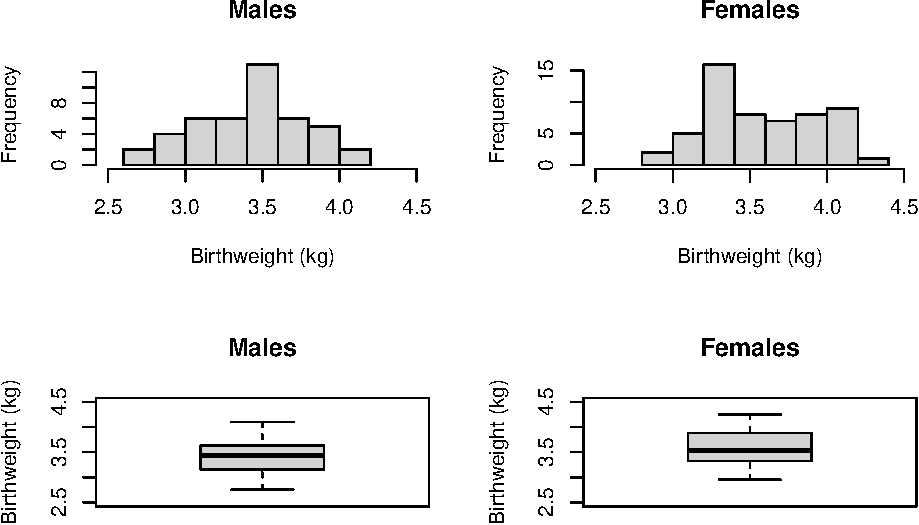
\includegraphics{phcm9795-R-notes_files/figure-latex/unnamed-chunk-68-1.pdf}

\begin{Shaded}
\begin{Highlighting}[]
\FunctionTok{par}\NormalTok{(}\AttributeTok{mfrow=}\FunctionTok{c}\NormalTok{(}\DecValTok{1}\NormalTok{,}\DecValTok{1}\NormalTok{))}
\end{Highlighting}
\end{Shaded}

To produce separate histograms in \texttt{ggplot2}, we use the \texttt{facet\_wrap} function to create a grid of plots. We can define the variable(s) to be plotted by in the \texttt{vars()}, and optionally, the number of rows (\texttt{nrow=}) and number of columns (\texttt{ncol=}).

\begin{Shaded}
\begin{Highlighting}[]
\CommentTok{\# Overall histogram of birthweight}
\FunctionTok{ggplot}\NormalTok{(bwt, }\FunctionTok{aes}\NormalTok{(}\AttributeTok{x=}\NormalTok{birthweight)) }\SpecialCharTok{+} 
  \FunctionTok{geom\_histogram}\NormalTok{(}\AttributeTok{breaks=}\FunctionTok{seq}\NormalTok{(}\FloatTok{2.5}\NormalTok{, }\FloatTok{4.5}\NormalTok{, }\FloatTok{0.25}\NormalTok{), }\AttributeTok{colour=}\StringTok{"black"}\NormalTok{, }\AttributeTok{fill=}\StringTok{"grey"}\NormalTok{) }\SpecialCharTok{+} 
  \FunctionTok{labs}\NormalTok{(}\AttributeTok{x=}\StringTok{"Birthweight (kg)"}\NormalTok{, }\AttributeTok{y=}\StringTok{"Frequency"}\NormalTok{) }\SpecialCharTok{+}
  \FunctionTok{theme\_classic}\NormalTok{()}
\end{Highlighting}
\end{Shaded}

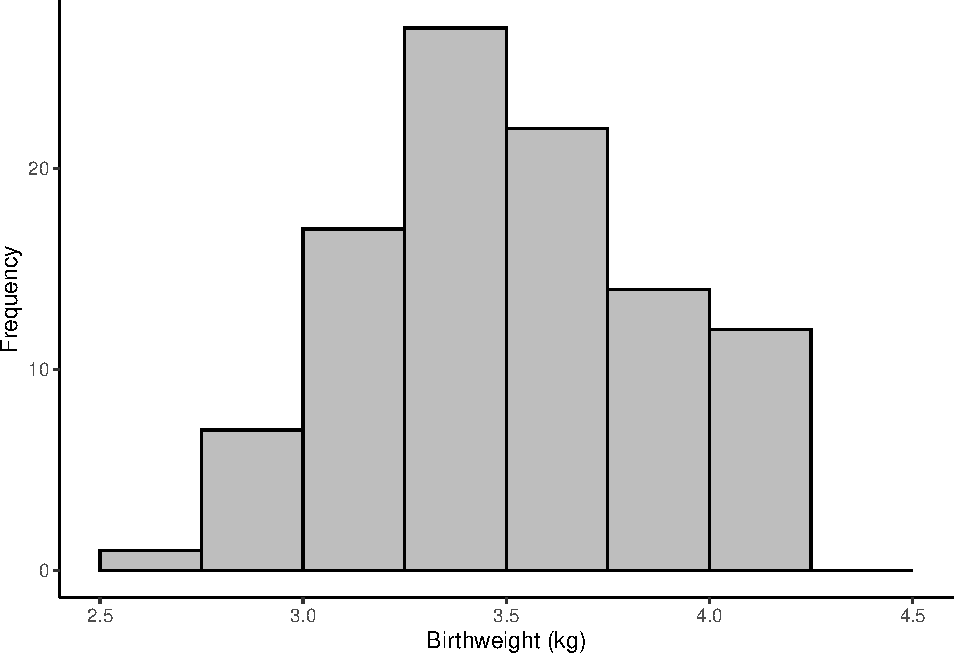
\includegraphics{phcm9795-R-notes_files/figure-latex/unnamed-chunk-69-1.pdf}

\begin{Shaded}
\begin{Highlighting}[]
\CommentTok{\# Histogram by gender}
\FunctionTok{ggplot}\NormalTok{(bwt, }\FunctionTok{aes}\NormalTok{(}\AttributeTok{x=}\NormalTok{birthweight)) }\SpecialCharTok{+} 
  \FunctionTok{geom\_histogram}\NormalTok{(}\AttributeTok{breaks=}\FunctionTok{seq}\NormalTok{(}\FloatTok{2.5}\NormalTok{, }\FloatTok{4.5}\NormalTok{, }\FloatTok{0.25}\NormalTok{), }\AttributeTok{colour=}\StringTok{"black"}\NormalTok{, }\AttributeTok{fill=}\StringTok{"grey"}\NormalTok{) }\SpecialCharTok{+} 
  \FunctionTok{facet\_wrap}\NormalTok{(}\FunctionTok{vars}\NormalTok{(gender), }\AttributeTok{nrow=}\DecValTok{1}\NormalTok{, }\AttributeTok{ncol=}\DecValTok{2}\NormalTok{) }\SpecialCharTok{+}
  \FunctionTok{labs}\NormalTok{(}\AttributeTok{x=}\StringTok{"Birthweight (kg)"}\NormalTok{, }\AttributeTok{y=}\StringTok{"Frequency"}\NormalTok{) }\SpecialCharTok{+}
  \FunctionTok{theme\_classic}\NormalTok{()}
\end{Highlighting}
\end{Shaded}

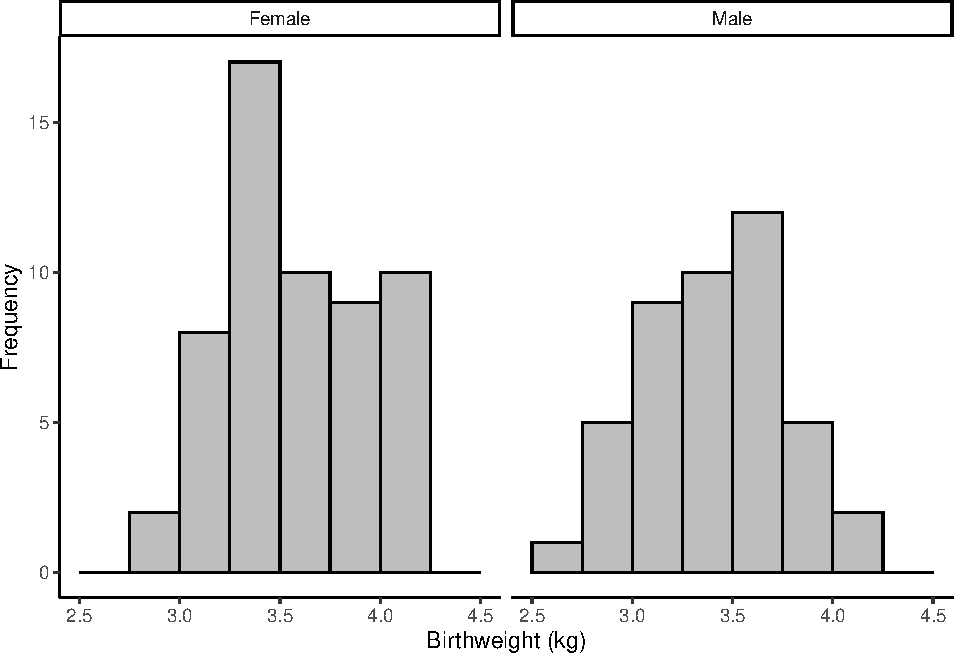
\includegraphics{phcm9795-R-notes_files/figure-latex/unnamed-chunk-69-2.pdf}

While it is possible to use \texttt{facet\_wrap} to produce separate boxplots, we can use the fact that the boxplot allows an \texttt{x} variable to be assigned to the ggplot aesthetic. By defining \texttt{birthweight} as the \texttt{y} variable and \texttt{gender} as the \texttt{x} variable, we can produce two boxplots in the same figure:

\begin{Shaded}
\begin{Highlighting}[]
\FunctionTok{ggplot}\NormalTok{(bwt, }\FunctionTok{aes}\NormalTok{(}\AttributeTok{x=}\NormalTok{gender, }\AttributeTok{y=}\NormalTok{birthweight)) }\SpecialCharTok{+}
  \FunctionTok{geom\_boxplot}\NormalTok{() }\SpecialCharTok{+}
  \FunctionTok{labs}\NormalTok{(}\AttributeTok{y=}\StringTok{"Birthweight (kg)"}\NormalTok{, }\AttributeTok{x=}\StringTok{"Gender"}\NormalTok{) }\SpecialCharTok{+}
  \FunctionTok{theme\_classic}\NormalTok{()}
\end{Highlighting}
\end{Shaded}

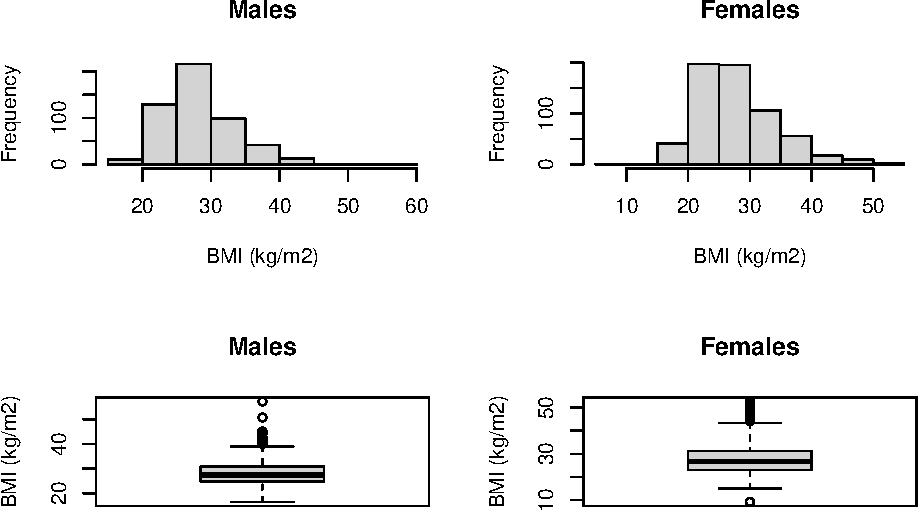
\includegraphics{phcm9795-R-notes_files/figure-latex/unnamed-chunk-70-1.pdf}

\hypertarget{producing-split-summary-statistics}{%
\subsection{Producing split summary statistics}\label{producing-split-summary-statistics}}

The \texttt{descriptives} function within the \texttt{jmv} function allows summary statistics to be calculated within subgroups using the \texttt{splitBy} argument:

\begin{Shaded}
\begin{Highlighting}[]
\FunctionTok{descriptives}\NormalTok{(}\AttributeTok{data=}\NormalTok{bwt, }\AttributeTok{vars=}\NormalTok{birthweight, }\AttributeTok{splitBy=}\NormalTok{gender)}
\end{Highlighting}
\end{Shaded}

\begin{verbatim}
## 
##  DESCRIPTIVES
## 
##  Descriptives                                    
##  ─────────────────────────────────────────────── 
##                          gender    birthweight   
##  ─────────────────────────────────────────────── 
##    N                     Female             56   
##                          Male               44   
##    Missing               Female              0   
##                          Male                0   
##    Mean                  Female       3.587411   
##                          Male         3.421364   
##    Median                Female       3.530000   
##                          Male         3.430000   
##    Standard deviation    Female      0.3629788   
##                          Male        0.3536165   
##    Minimum               Female       2.950000   
##                          Male         2.750000   
##    Maximum               Female       4.250000   
##                          Male         4.100000   
##  ───────────────────────────────────────────────
\end{verbatim}

\hypertarget{independent-samples-t-test}{%
\section{Independent samples t-test}\label{independent-samples-t-test}}

\begin{Shaded}
\begin{Highlighting}[]
\FunctionTok{ttestIS}\NormalTok{(}\AttributeTok{data=}\NormalTok{bwt, }\AttributeTok{vars=}\NormalTok{birthweight, }\AttributeTok{group=}\NormalTok{gender)}
\end{Highlighting}
\end{Shaded}

INDEPENDENT SAMPLES T-TEST

Independent Samples T-Test\\
────────────────────────────────────────────────────────────────────
Statistic df p\\
────────────────────────────────────────────────────────────────────
birthweight Student's t 2.296556 98.00000 0.0237731\\
────────────────────────────────────────────────────────────────────

\begin{Shaded}
\begin{Highlighting}[]
\FunctionTok{ttestIS}\NormalTok{(}\AttributeTok{data=}\NormalTok{bwt, }\AttributeTok{vars=}\NormalTok{birthweight, }\AttributeTok{group=}\NormalTok{gender, }\AttributeTok{meanDiff=}\ConstantTok{TRUE}\NormalTok{, }\AttributeTok{ci=}\ConstantTok{TRUE}\NormalTok{)}
\end{Highlighting}
\end{Shaded}

INDEPENDENT SAMPLES T-TEST

Independent Samples T-Test\\
───────────────────────────────────────────────────────────────────────────────────────────────────────────────────────────────────
Statistic df p Mean difference SE difference Lower Upper\\
───────────────────────────────────────────────────────────────────────────────────────────────────────────────────────────────────
birthweight Student's t 2.296556 98.00000 0.0237731 0.1660471 0.07230265 0.02256481 0.3095293\\
───────────────────────────────────────────────────────────────────────────────────────────────────────────────────────────────────

\begin{Shaded}
\begin{Highlighting}[]
\FunctionTok{ttestIS}\NormalTok{(}\AttributeTok{data=}\NormalTok{bwt, }\AttributeTok{vars=}\NormalTok{birthweight, }\AttributeTok{group=}\NormalTok{gender, }\AttributeTok{meanDiff=}\ConstantTok{TRUE}\NormalTok{, }\AttributeTok{ci=}\ConstantTok{TRUE}\NormalTok{, }\AttributeTok{welchs=}\ConstantTok{TRUE}\NormalTok{)}
\end{Highlighting}
\end{Shaded}

INDEPENDENT SAMPLES T-TEST

Independent Samples T-Test\\
───────────────────────────────────────────────────────────────────────────────────────────────────────────────────────────────────
Statistic df p Mean difference SE difference Lower Upper\\
───────────────────────────────────────────────────────────────────────────────────────────────────────────────────────────────────
birthweight Student's t 2.296556 98.00000 0.0237731 0.1660471 0.07230265 0.02256481 0.3095293\\
Welch's t 2.303840 93.54377 0.0234458 0.1660471 0.07207403 0.02293328 0.3091609\\
───────────────────────────────────────────────────────────────────────────────────────────────────────────────────────────────────

\hypertarget{checking-the-assumptions-for-a-paired-t-test}{%
\section{Checking the assumptions for a Paired t-test}\label{checking-the-assumptions-for-a-paired-t-test}}

Before performing a paired t-test, you must check that the assumptions for the test have been met. Using the dataset \texttt{Example\_5.2.dta} to show that the difference between the pair of measurements between the sites is normally distributed, we first need to compute a new variable of the differences and examine its histogram.

\begin{Shaded}
\begin{Highlighting}[]
\NormalTok{sbp }\OtherTok{\textless{}{-}} \FunctionTok{read\_dta}\NormalTok{(}\StringTok{"/Users/td/Documents/GithubRepos/phcm9795/data/examples/Example\_5.2.dta"}\NormalTok{)}
\NormalTok{sbp}\SpecialCharTok{$}\NormalTok{diff }\OtherTok{=}\NormalTok{ sbp}\SpecialCharTok{$}\NormalTok{sbp\_dp }\SpecialCharTok{{-}}\NormalTok{ sbp}\SpecialCharTok{$}\NormalTok{sbp\_tp}
\FunctionTok{hist}\NormalTok{(sbp}\SpecialCharTok{$}\NormalTok{diff, }\AttributeTok{xlab=}\StringTok{"Blood pressure (mmHg)"}\NormalTok{, }\AttributeTok{main=}\StringTok{"Difference in systolic blood pressure"}\NormalTok{)}
\end{Highlighting}
\end{Shaded}

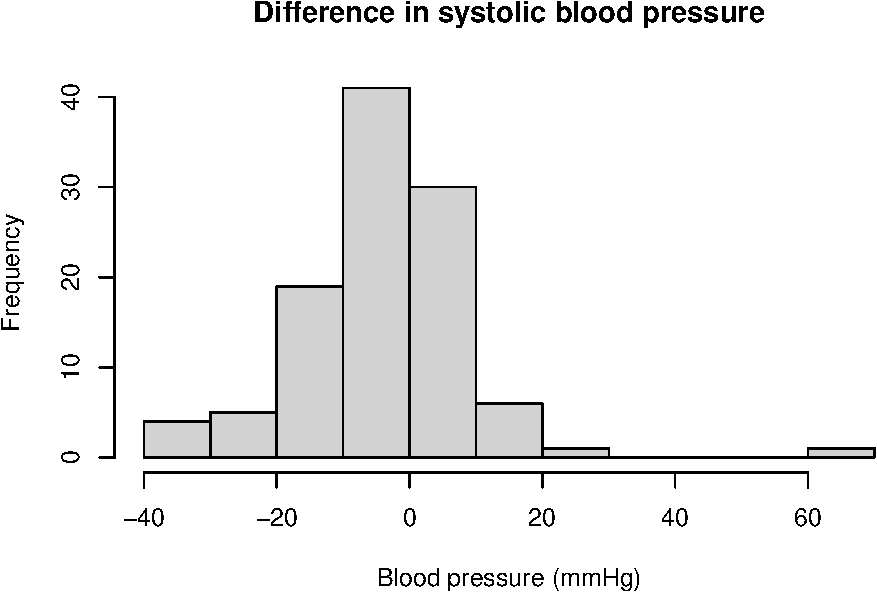
\includegraphics{phcm9795-R-notes_files/figure-latex/unnamed-chunk-73-1.pdf}

\hypertarget{paired-t-test}{%
\section{Paired t-Test}\label{paired-t-test}}

To perform a paired t-test we will use the dataset \texttt{Example\_5.2.dta}.

\begin{Shaded}
\begin{Highlighting}[]
\FunctionTok{ttestPS}\NormalTok{(}\AttributeTok{data=}\NormalTok{sbp, }\AttributeTok{pairs=}\FunctionTok{list}\NormalTok{(}\FunctionTok{list}\NormalTok{(}\AttributeTok{i1 =} \StringTok{\textquotesingle{}sbp\_dp\textquotesingle{}}\NormalTok{, }\AttributeTok{i2 =} \StringTok{\textquotesingle{}sbp\_tp\textquotesingle{}}\NormalTok{)), }\AttributeTok{meanDiff=}\ConstantTok{TRUE}\NormalTok{, }\AttributeTok{ci=}\ConstantTok{TRUE}\NormalTok{)}
\end{Highlighting}
\end{Shaded}

\begin{verbatim}
## 
##  PAIRED SAMPLES T-TEST
## 
##  Paired Samples T-Test                                                                                                                   
##  ─────────────────────────────────────────────────────────────────────────────────────────────────────────────────────────────────────── 
##                                       statistic     df          p            Mean difference    SE difference    Lower        Upper      
##  ─────────────────────────────────────────────────────────────────────────────────────────────────────────────────────────────────────── 
##    sbp_dp    sbp_tp    Student's t    -0.9621117    106.0000    0.3381832          -1.261682         1.311368    -3.861596    1.338232   
##  ───────────────────────────────────────────────────────────────────────────────────────────────────────────────────────────────────────
\end{verbatim}

The syntax of the ttestPS function is a little cumbersome. The \texttt{t.test} function can be used as an alternative:

\begin{Shaded}
\begin{Highlighting}[]
\FunctionTok{t.test}\NormalTok{(sbp}\SpecialCharTok{$}\NormalTok{sbp\_dp, sbp}\SpecialCharTok{$}\NormalTok{sbp\_tp, }\AttributeTok{paired=}\ConstantTok{TRUE}\NormalTok{)}
\end{Highlighting}
\end{Shaded}

\begin{verbatim}
## 
##  Paired t-test
## 
## data:  sbp$sbp_dp and sbp$sbp_tp
## t = -0.96211, df = 106, p-value = 0.3382
## alternative hypothesis: true difference in means is not equal to 0
## 95 percent confidence interval:
##  -3.861596  1.338232
## sample estimates:
## mean of the differences 
##               -1.261682
\end{verbatim}

\hypertarget{proportions}{%
\chapter{Proportions}\label{proportions}}

\hypertarget{confidence-intervals-for-proportions}{%
\section{95\% confidence intervals for proportions}\label{confidence-intervals-for-proportions}}

We can use the \texttt{BinomCI(x=,\ n=,\ method=)} function within the \texttt{DescTools} package to compute 95\% confidence intervals for proportions. Here we specify \texttt{x}: the number of successes, \texttt{n}: the sample size, and optionally, the \texttt{method} (which defaults to Wilson's method).

\begin{Shaded}
\begin{Highlighting}[]
\FunctionTok{library}\NormalTok{(DescTools)}

\FunctionTok{BinomCI}\NormalTok{(}\AttributeTok{x=}\DecValTok{47}\NormalTok{, }\AttributeTok{n=}\DecValTok{215}\NormalTok{, }\AttributeTok{method=}\StringTok{\textquotesingle{}wald\textquotesingle{}}\NormalTok{)}
\end{Highlighting}
\end{Shaded}

\begin{verbatim}
##            est    lwr.ci    upr.ci
## [1,] 0.2186047 0.1633595 0.2738498
\end{verbatim}

\begin{Shaded}
\begin{Highlighting}[]
\FunctionTok{BinomCI}\NormalTok{(}\AttributeTok{x=}\DecValTok{47}\NormalTok{, }\AttributeTok{n=}\DecValTok{215}\NormalTok{, }\AttributeTok{method=}\StringTok{\textquotesingle{}wilson\textquotesingle{}}\NormalTok{)}
\end{Highlighting}
\end{Shaded}

\begin{verbatim}
##            est    lwr.ci    upr.ci
## [1,] 0.2186047 0.1685637 0.2785246
\end{verbatim}

\hypertarget{significance-test-for-single-proportion}{%
\section{Significance test for single proportion}\label{significance-test-for-single-proportion}}

We can use the \texttt{binom.test} function to perform a significance test for a single proportion: \texttt{binom.test(x=,\ n=,\ p=)}. Here we specify \texttt{x}: the number of successes, \texttt{n}: the sample size, and \texttt{p}: the hypothesised proportion (which defaults to 0.5 if nothing is entered).

\begin{Shaded}
\begin{Highlighting}[]
\FunctionTok{binom.test}\NormalTok{(}\AttributeTok{x=}\DecValTok{54}\NormalTok{, }\AttributeTok{n=}\DecValTok{300}\NormalTok{, }\AttributeTok{p=}\FloatTok{0.2}\NormalTok{)}
\end{Highlighting}
\end{Shaded}

\begin{verbatim}
## 
##  Exact binomial test
## 
## data:  54 and 300
## number of successes = 54, number of trials = 300, p-value = 0.4273
## alternative hypothesis: true probability of success is not equal to 0.2
## 95 percent confidence interval:
##  0.1382104 0.2282394
## sample estimates:
## probability of success 
##                   0.18
\end{verbatim}

\hypertarget{computing-a-relative-risk-and-its-95-confidence-interval}{%
\section{Computing a relative risk and its 95\% confidence interval}\label{computing-a-relative-risk-and-its-95-confidence-interval}}

\begin{Shaded}
\begin{Highlighting}[]
\FunctionTok{library}\NormalTok{(haven)}
\FunctionTok{library}\NormalTok{(labelled)}
\FunctionTok{library}\NormalTok{(jmv)}

\NormalTok{drug }\OtherTok{\textless{}{-}} \FunctionTok{read\_dta}\NormalTok{(}\StringTok{"/Users/td/Documents/GithubRepos/phcm9795/data/examples/Example\_6.4.dta"}\NormalTok{) }\SpecialCharTok{\%\textgreater{}\%} 
  \FunctionTok{unlabelled}\NormalTok{()}

\FunctionTok{head}\NormalTok{(drug)}
\end{Highlighting}
\end{Shaded}

 
  \providecommand{\huxb}[2]{\arrayrulecolor[RGB]{#1}\global\arrayrulewidth=#2pt}
  \providecommand{\huxvb}[2]{\color[RGB]{#1}\vrule width #2pt}
  \providecommand{\huxtpad}[1]{\rule{0pt}{#1}}
  \providecommand{\huxbpad}[1]{\rule[-#1]{0pt}{#1}}

\begin{table}[ht]
\begin{centerbox}
\begin{threeparttable}
\captionsetup{justification=centering,singlelinecheck=off}
\caption{\label{tab:unnamed-chunk-78} }
 \setlength{\tabcolsep}{0pt}
\begin{tabular}{l l}


\hhline{>{\huxb{0, 0, 0}{0.4}}->{\huxb{0, 0, 0}{0.4}}-}
\arrayrulecolor{black}

\multicolumn{1}{!{\huxvb{0, 0, 0}{0.4}}l!{\huxvb{0, 0, 0}{0}}}{\huxtpad{6pt + 1em}\raggedright \hspace{6pt} \textbf{group} \hspace{6pt}\huxbpad{6pt}} &
\multicolumn{1}{l!{\huxvb{0, 0, 0}{0.4}}}{\huxtpad{6pt + 1em}\raggedright \hspace{6pt} \textbf{side\_effect} \hspace{6pt}\huxbpad{6pt}} \tabularnewline[-0.5pt]


\hhline{>{\huxb{0, 0, 0}{0.4}}->{\huxb{0, 0, 0}{0.4}}-}
\arrayrulecolor{black}

\multicolumn{1}{!{\huxvb{0, 0, 0}{0.4}}l!{\huxvb{0, 0, 0}{0}}}{\cellcolor[RGB]{242, 242, 242}\huxtpad{6pt + 1em}\raggedright \hspace{6pt} Placebo \hspace{6pt}\huxbpad{6pt}} &
\multicolumn{1}{l!{\huxvb{0, 0, 0}{0.4}}}{\cellcolor[RGB]{242, 242, 242}\huxtpad{6pt + 1em}\raggedright \hspace{6pt} Nausea \hspace{6pt}\huxbpad{6pt}} \tabularnewline[-0.5pt]


\hhline{>{\huxb{0, 0, 0}{0.4}}|>{\huxb{0, 0, 0}{0.4}}|}
\arrayrulecolor{black}

\multicolumn{1}{!{\huxvb{0, 0, 0}{0.4}}l!{\huxvb{0, 0, 0}{0}}}{\huxtpad{6pt + 1em}\raggedright \hspace{6pt} Placebo \hspace{6pt}\huxbpad{6pt}} &
\multicolumn{1}{l!{\huxvb{0, 0, 0}{0.4}}}{\huxtpad{6pt + 1em}\raggedright \hspace{6pt} Nausea \hspace{6pt}\huxbpad{6pt}} \tabularnewline[-0.5pt]


\hhline{>{\huxb{0, 0, 0}{0.4}}|>{\huxb{0, 0, 0}{0.4}}|}
\arrayrulecolor{black}

\multicolumn{1}{!{\huxvb{0, 0, 0}{0.4}}l!{\huxvb{0, 0, 0}{0}}}{\cellcolor[RGB]{242, 242, 242}\huxtpad{6pt + 1em}\raggedright \hspace{6pt} Placebo \hspace{6pt}\huxbpad{6pt}} &
\multicolumn{1}{l!{\huxvb{0, 0, 0}{0.4}}}{\cellcolor[RGB]{242, 242, 242}\huxtpad{6pt + 1em}\raggedright \hspace{6pt} Nausea \hspace{6pt}\huxbpad{6pt}} \tabularnewline[-0.5pt]


\hhline{>{\huxb{0, 0, 0}{0.4}}|>{\huxb{0, 0, 0}{0.4}}|}
\arrayrulecolor{black}

\multicolumn{1}{!{\huxvb{0, 0, 0}{0.4}}l!{\huxvb{0, 0, 0}{0}}}{\huxtpad{6pt + 1em}\raggedright \hspace{6pt} Placebo \hspace{6pt}\huxbpad{6pt}} &
\multicolumn{1}{l!{\huxvb{0, 0, 0}{0.4}}}{\huxtpad{6pt + 1em}\raggedright \hspace{6pt} Nausea \hspace{6pt}\huxbpad{6pt}} \tabularnewline[-0.5pt]


\hhline{>{\huxb{0, 0, 0}{0.4}}|>{\huxb{0, 0, 0}{0.4}}|}
\arrayrulecolor{black}

\multicolumn{1}{!{\huxvb{0, 0, 0}{0.4}}l!{\huxvb{0, 0, 0}{0}}}{\cellcolor[RGB]{242, 242, 242}\huxtpad{6pt + 1em}\raggedright \hspace{6pt} Placebo \hspace{6pt}\huxbpad{6pt}} &
\multicolumn{1}{l!{\huxvb{0, 0, 0}{0.4}}}{\cellcolor[RGB]{242, 242, 242}\huxtpad{6pt + 1em}\raggedright \hspace{6pt} No nausea \hspace{6pt}\huxbpad{6pt}} \tabularnewline[-0.5pt]


\hhline{>{\huxb{0, 0, 0}{0.4}}|>{\huxb{0, 0, 0}{0.4}}|}
\arrayrulecolor{black}

\multicolumn{1}{!{\huxvb{0, 0, 0}{0.4}}l!{\huxvb{0, 0, 0}{0}}}{\huxtpad{6pt + 1em}\raggedright \hspace{6pt} Placebo \hspace{6pt}\huxbpad{6pt}} &
\multicolumn{1}{l!{\huxvb{0, 0, 0}{0.4}}}{\huxtpad{6pt + 1em}\raggedright \hspace{6pt} No nausea \hspace{6pt}\huxbpad{6pt}} \tabularnewline[-0.5pt]


\hhline{>{\huxb{0, 0, 0}{0.4}}->{\huxb{0, 0, 0}{0.4}}-}
\arrayrulecolor{black}
\end{tabular}
\end{threeparttable}\par\end{centerbox}

\end{table}
 

\begin{Shaded}
\begin{Highlighting}[]
\FunctionTok{table}\NormalTok{(drug}\SpecialCharTok{$}\NormalTok{group)}
\end{Highlighting}
\end{Shaded}

\begin{verbatim}
## 
## Placebo  Active 
##      50      50
\end{verbatim}

\begin{Shaded}
\begin{Highlighting}[]
\FunctionTok{table}\NormalTok{(drug}\SpecialCharTok{$}\NormalTok{side\_effect)}
\end{Highlighting}
\end{Shaded}

\begin{verbatim}
## 
## No nausea    Nausea 
##        81        19
\end{verbatim}

\begin{Shaded}
\begin{Highlighting}[]
\FunctionTok{table}\NormalTok{(drug}\SpecialCharTok{$}\NormalTok{group, drug}\SpecialCharTok{$}\NormalTok{side\_effect)}
\end{Highlighting}
\end{Shaded}

\begin{verbatim}
##          
##           No nausea Nausea
##   Placebo        46      4
##   Active         35     15
\end{verbatim}

\begin{Shaded}
\begin{Highlighting}[]
\NormalTok{drug}\SpecialCharTok{$}\NormalTok{group }\OtherTok{\textless{}{-}} \FunctionTok{relevel}\NormalTok{(drug}\SpecialCharTok{$}\NormalTok{group, }\AttributeTok{ref=}\StringTok{"Active"}\NormalTok{)}
\NormalTok{drug}\SpecialCharTok{$}\NormalTok{side\_effect }\OtherTok{\textless{}{-}} \FunctionTok{relevel}\NormalTok{(drug}\SpecialCharTok{$}\NormalTok{side\_effect, }\AttributeTok{ref=}\StringTok{"Nausea"}\NormalTok{)}

\FunctionTok{table}\NormalTok{(drug}\SpecialCharTok{$}\NormalTok{group)}
\end{Highlighting}
\end{Shaded}

\begin{verbatim}
## 
##  Active Placebo 
##      50      50
\end{verbatim}

\begin{Shaded}
\begin{Highlighting}[]
\FunctionTok{table}\NormalTok{(drug}\SpecialCharTok{$}\NormalTok{side\_effect)}
\end{Highlighting}
\end{Shaded}

\begin{verbatim}
## 
##    Nausea No nausea 
##        19        81
\end{verbatim}

\begin{Shaded}
\begin{Highlighting}[]
\FunctionTok{table}\NormalTok{(drug}\SpecialCharTok{$}\NormalTok{group, drug}\SpecialCharTok{$}\NormalTok{side\_effect)}
\end{Highlighting}
\end{Shaded}

\begin{verbatim}
##          
##           Nausea No nausea
##   Active      15        35
##   Placebo      4        46
\end{verbatim}

\begin{Shaded}
\begin{Highlighting}[]
\FunctionTok{contTables}\NormalTok{(}\AttributeTok{data=}\NormalTok{drug, }\AttributeTok{rows=}\NormalTok{group, }\AttributeTok{cols=}\NormalTok{side\_effect, }\AttributeTok{pcRow=}\ConstantTok{TRUE}\NormalTok{, }\AttributeTok{relRisk =} \ConstantTok{TRUE}\NormalTok{, }\AttributeTok{diffProp =} \ConstantTok{TRUE}\NormalTok{)}
\end{Highlighting}
\end{Shaded}

\begin{verbatim}
## 
##  CONTINGENCY TABLES
## 
##  Contingency Tables                                                 
##  ────────────────────────────────────────────────────────────────── 
##    group                      Nausea       No nausea    Total       
##  ────────────────────────────────────────────────────────────────── 
##    Active     Observed               15           35           50   
##               % within row     30.00000     70.00000    100.00000   
##                                                                     
##    Placebo    Observed                4           46           50   
##               % within row      8.00000     92.00000    100.00000   
##                                                                     
##    Total      Observed               19           81          100   
##               % within row     19.00000     81.00000    100.00000   
##  ────────────────────────────────────────────────────────────────── 
## 
## 
##  χ² Tests                              
##  ───────────────────────────────────── 
##          Value       df    p           
##  ───────────────────────────────────── 
##    χ²    7.862248     1    0.0050478   
##    N          100                      
##  ───────────────────────────────────── 
## 
## 
##  Comparative Measures                                                    
##  ─────────────────────────────────────────────────────────────────────── 
##                                   Value        Lower         Upper       
##  ─────────────────────────────────────────────────────────────────────── 
##    Difference in 2 proportions    0.2200000    0.07238986    0.3676101   
##    Relative risk                   3.750000      1.337540     10.51370   
##  ───────────────────────────────────────────────────────────────────────
\end{verbatim}

If you only have the cross-tabulated data (i.e.~aggregated), you will need to enter your data into a new data frame.

\begin{Shaded}
\begin{Highlighting}[]
\NormalTok{drug\_aggregated }\OtherTok{\textless{}{-}} \FunctionTok{data.frame}\NormalTok{(}
  \AttributeTok{group =} \FunctionTok{c}\NormalTok{(}\DecValTok{1}\NormalTok{, }\DecValTok{1}\NormalTok{, }\DecValTok{0}\NormalTok{, }\DecValTok{0}\NormalTok{),}
  \AttributeTok{side\_effect =} \FunctionTok{c}\NormalTok{(}\DecValTok{1}\NormalTok{, }\DecValTok{0}\NormalTok{, }\DecValTok{1}\NormalTok{, }\DecValTok{0}\NormalTok{),}
  \AttributeTok{n =} \FunctionTok{c}\NormalTok{(}\DecValTok{15}\NormalTok{, }\DecValTok{35}\NormalTok{, }\DecValTok{4}\NormalTok{, }\DecValTok{46}\NormalTok{)}
\NormalTok{)}

\NormalTok{drug\_aggregated}\SpecialCharTok{$}\NormalTok{group }\OtherTok{\textless{}{-}} \FunctionTok{factor}\NormalTok{(drug\_aggregated}\SpecialCharTok{$}\NormalTok{group, }\AttributeTok{levels=}\FunctionTok{c}\NormalTok{(}\DecValTok{1}\NormalTok{,}\DecValTok{0}\NormalTok{), }\AttributeTok{labels=}\FunctionTok{c}\NormalTok{(}\StringTok{"Active"}\NormalTok{, }\StringTok{"Placebo"}\NormalTok{))}
\NormalTok{drug\_aggregated}\SpecialCharTok{$}\NormalTok{side\_effect }\OtherTok{\textless{}{-}} \FunctionTok{factor}\NormalTok{(drug\_aggregated}\SpecialCharTok{$}\NormalTok{side\_effect, }\AttributeTok{levels=}\FunctionTok{c}\NormalTok{(}\DecValTok{1}\NormalTok{,}\DecValTok{0}\NormalTok{), }\AttributeTok{labels=}\FunctionTok{c}\NormalTok{(}\StringTok{"Nausea"}\NormalTok{, }\StringTok{"No nausea"}\NormalTok{))}

\NormalTok{drug\_aggregated}
\end{Highlighting}
\end{Shaded}

 
  \providecommand{\huxb}[2]{\arrayrulecolor[RGB]{#1}\global\arrayrulewidth=#2pt}
  \providecommand{\huxvb}[2]{\color[RGB]{#1}\vrule width #2pt}
  \providecommand{\huxtpad}[1]{\rule{0pt}{#1}}
  \providecommand{\huxbpad}[1]{\rule[-#1]{0pt}{#1}}

\begin{table}[ht]
\begin{centerbox}
\begin{threeparttable}
\captionsetup{justification=centering,singlelinecheck=off}
\caption{\label{tab:unnamed-chunk-79} }
 \setlength{\tabcolsep}{0pt}
\begin{tabular}{l l l}


\hhline{>{\huxb{0, 0, 0}{0.4}}->{\huxb{0, 0, 0}{0.4}}->{\huxb{0, 0, 0}{0.4}}-}
\arrayrulecolor{black}

\multicolumn{1}{!{\huxvb{0, 0, 0}{0.4}}l!{\huxvb{0, 0, 0}{0}}}{\huxtpad{6pt + 1em}\raggedright \hspace{6pt} \textbf{group} \hspace{6pt}\huxbpad{6pt}} &
\multicolumn{1}{l!{\huxvb{0, 0, 0}{0}}}{\huxtpad{6pt + 1em}\raggedright \hspace{6pt} \textbf{side\_effect} \hspace{6pt}\huxbpad{6pt}} &
\multicolumn{1}{r!{\huxvb{0, 0, 0}{0.4}}}{\huxtpad{6pt + 1em}\raggedleft \hspace{6pt} \textbf{n} \hspace{6pt}\huxbpad{6pt}} \tabularnewline[-0.5pt]


\hhline{>{\huxb{0, 0, 0}{0.4}}->{\huxb{0, 0, 0}{0.4}}->{\huxb{0, 0, 0}{0.4}}-}
\arrayrulecolor{black}

\multicolumn{1}{!{\huxvb{0, 0, 0}{0.4}}l!{\huxvb{0, 0, 0}{0}}}{\cellcolor[RGB]{242, 242, 242}\huxtpad{6pt + 1em}\raggedright \hspace{6pt} Active \hspace{6pt}\huxbpad{6pt}} &
\multicolumn{1}{l!{\huxvb{0, 0, 0}{0}}}{\cellcolor[RGB]{242, 242, 242}\huxtpad{6pt + 1em}\raggedright \hspace{6pt} Nausea \hspace{6pt}\huxbpad{6pt}} &
\multicolumn{1}{r!{\huxvb{0, 0, 0}{0.4}}}{\cellcolor[RGB]{242, 242, 242}\huxtpad{6pt + 1em}\raggedleft \hspace{6pt} 15 \hspace{6pt}\huxbpad{6pt}} \tabularnewline[-0.5pt]


\hhline{>{\huxb{0, 0, 0}{0.4}}|>{\huxb{0, 0, 0}{0.4}}|}
\arrayrulecolor{black}

\multicolumn{1}{!{\huxvb{0, 0, 0}{0.4}}l!{\huxvb{0, 0, 0}{0}}}{\huxtpad{6pt + 1em}\raggedright \hspace{6pt} Active \hspace{6pt}\huxbpad{6pt}} &
\multicolumn{1}{l!{\huxvb{0, 0, 0}{0}}}{\huxtpad{6pt + 1em}\raggedright \hspace{6pt} No nausea \hspace{6pt}\huxbpad{6pt}} &
\multicolumn{1}{r!{\huxvb{0, 0, 0}{0.4}}}{\huxtpad{6pt + 1em}\raggedleft \hspace{6pt} 35 \hspace{6pt}\huxbpad{6pt}} \tabularnewline[-0.5pt]


\hhline{>{\huxb{0, 0, 0}{0.4}}|>{\huxb{0, 0, 0}{0.4}}|}
\arrayrulecolor{black}

\multicolumn{1}{!{\huxvb{0, 0, 0}{0.4}}l!{\huxvb{0, 0, 0}{0}}}{\cellcolor[RGB]{242, 242, 242}\huxtpad{6pt + 1em}\raggedright \hspace{6pt} Placebo \hspace{6pt}\huxbpad{6pt}} &
\multicolumn{1}{l!{\huxvb{0, 0, 0}{0}}}{\cellcolor[RGB]{242, 242, 242}\huxtpad{6pt + 1em}\raggedright \hspace{6pt} Nausea \hspace{6pt}\huxbpad{6pt}} &
\multicolumn{1}{r!{\huxvb{0, 0, 0}{0.4}}}{\cellcolor[RGB]{242, 242, 242}\huxtpad{6pt + 1em}\raggedleft \hspace{6pt} 4 \hspace{6pt}\huxbpad{6pt}} \tabularnewline[-0.5pt]


\hhline{>{\huxb{0, 0, 0}{0.4}}|>{\huxb{0, 0, 0}{0.4}}|}
\arrayrulecolor{black}

\multicolumn{1}{!{\huxvb{0, 0, 0}{0.4}}l!{\huxvb{0, 0, 0}{0}}}{\huxtpad{6pt + 1em}\raggedright \hspace{6pt} Placebo \hspace{6pt}\huxbpad{6pt}} &
\multicolumn{1}{l!{\huxvb{0, 0, 0}{0}}}{\huxtpad{6pt + 1em}\raggedright \hspace{6pt} No nausea \hspace{6pt}\huxbpad{6pt}} &
\multicolumn{1}{r!{\huxvb{0, 0, 0}{0.4}}}{\huxtpad{6pt + 1em}\raggedleft \hspace{6pt} 46 \hspace{6pt}\huxbpad{6pt}} \tabularnewline[-0.5pt]


\hhline{>{\huxb{0, 0, 0}{0.4}}->{\huxb{0, 0, 0}{0.4}}->{\huxb{0, 0, 0}{0.4}}-}
\arrayrulecolor{black}
\end{tabular}
\end{threeparttable}\par\end{centerbox}

\end{table}
 

\begin{Shaded}
\begin{Highlighting}[]
\FunctionTok{contTables}\NormalTok{(}\AttributeTok{data=}\NormalTok{drug\_aggregated, }\AttributeTok{rows=}\NormalTok{group, }\AttributeTok{cols=}\NormalTok{side\_effect, }\AttributeTok{count=}\NormalTok{n, }\AttributeTok{pcRow=}\ConstantTok{TRUE}\NormalTok{, }\AttributeTok{relRisk =} \ConstantTok{TRUE}\NormalTok{, }\AttributeTok{diffProp =} \ConstantTok{TRUE}\NormalTok{)}
\end{Highlighting}
\end{Shaded}

\begin{verbatim}
## 
##  CONTINGENCY TABLES
## 
##  Contingency Tables                                                 
##  ────────────────────────────────────────────────────────────────── 
##    group                      Nausea       No nausea    Total       
##  ────────────────────────────────────────────────────────────────── 
##    Active     Observed               15           35           50   
##               % within row     30.00000     70.00000    100.00000   
##                                                                     
##    Placebo    Observed                4           46           50   
##               % within row      8.00000     92.00000    100.00000   
##                                                                     
##    Total      Observed               19           81          100   
##               % within row     19.00000     81.00000    100.00000   
##  ────────────────────────────────────────────────────────────────── 
## 
## 
##  χ² Tests                              
##  ───────────────────────────────────── 
##          Value       df    p           
##  ───────────────────────────────────── 
##    χ²    7.862248     1    0.0050478   
##    N          100                      
##  ───────────────────────────────────── 
## 
## 
##  Comparative Measures                                                    
##  ─────────────────────────────────────────────────────────────────────── 
##                                   Value        Lower         Upper       
##  ─────────────────────────────────────────────────────────────────────── 
##    Difference in 2 proportions    0.2200000    0.07238986    0.3676101   
##    Relative risk                   3.750000      1.337540     10.51370   
##  ───────────────────────────────────────────────────────────────────────
\end{verbatim}

\hypertarget{computing-an-odds-ratio-and-its-95ci}{%
\section{Computing an odds ratio and its 95\%CI}\label{computing-an-odds-ratio-and-its-95ci}}

We can use the \texttt{contTables} function To obtain an odds ratio and its 95\% CI, by specifying \texttt{odds=TRUE}:

\begin{Shaded}
\begin{Highlighting}[]
\NormalTok{hpv }\OtherTok{\textless{}{-}} \FunctionTok{data.frame}\NormalTok{(}
  \AttributeTok{cancer =} \FunctionTok{c}\NormalTok{(}\DecValTok{1}\NormalTok{, }\DecValTok{1}\NormalTok{, }\DecValTok{0}\NormalTok{, }\DecValTok{0}\NormalTok{),}
  \AttributeTok{hpv =} \FunctionTok{c}\NormalTok{(}\DecValTok{1}\NormalTok{, }\DecValTok{0}\NormalTok{, }\DecValTok{1}\NormalTok{, }\DecValTok{0}\NormalTok{),}
  \AttributeTok{n =} \FunctionTok{c}\NormalTok{(}\DecValTok{57}\NormalTok{, }\DecValTok{14}\NormalTok{, }\DecValTok{43}\NormalTok{, }\DecValTok{186}\NormalTok{)}
\NormalTok{)}

\NormalTok{hpv}\SpecialCharTok{$}\NormalTok{cancer }\OtherTok{\textless{}{-}} \FunctionTok{factor}\NormalTok{(hpv}\SpecialCharTok{$}\NormalTok{cancer, }\AttributeTok{levels=}\FunctionTok{c}\NormalTok{(}\DecValTok{1}\NormalTok{,}\DecValTok{0}\NormalTok{), }\AttributeTok{labels=}\FunctionTok{c}\NormalTok{(}\StringTok{"Case"}\NormalTok{, }\StringTok{"Control"}\NormalTok{))}
\NormalTok{hpv}\SpecialCharTok{$}\NormalTok{hpv }\OtherTok{\textless{}{-}} \FunctionTok{factor}\NormalTok{(hpv}\SpecialCharTok{$}\NormalTok{hpv, }\AttributeTok{levels=}\FunctionTok{c}\NormalTok{(}\DecValTok{1}\NormalTok{,}\DecValTok{0}\NormalTok{), }\AttributeTok{labels=}\FunctionTok{c}\NormalTok{(}\StringTok{"HPV +"}\NormalTok{, }\StringTok{"HPV {-}"}\NormalTok{))}

\NormalTok{hpv}
\end{Highlighting}
\end{Shaded}

 
  \providecommand{\huxb}[2]{\arrayrulecolor[RGB]{#1}\global\arrayrulewidth=#2pt}
  \providecommand{\huxvb}[2]{\color[RGB]{#1}\vrule width #2pt}
  \providecommand{\huxtpad}[1]{\rule{0pt}{#1}}
  \providecommand{\huxbpad}[1]{\rule[-#1]{0pt}{#1}}

\begin{table}[ht]
\begin{centerbox}
\begin{threeparttable}
\captionsetup{justification=centering,singlelinecheck=off}
\caption{\label{tab:unnamed-chunk-80} }
 \setlength{\tabcolsep}{0pt}
\begin{tabular}{l l l}


\hhline{>{\huxb{0, 0, 0}{0.4}}->{\huxb{0, 0, 0}{0.4}}->{\huxb{0, 0, 0}{0.4}}-}
\arrayrulecolor{black}

\multicolumn{1}{!{\huxvb{0, 0, 0}{0.4}}l!{\huxvb{0, 0, 0}{0}}}{\huxtpad{6pt + 1em}\raggedright \hspace{6pt} \textbf{cancer} \hspace{6pt}\huxbpad{6pt}} &
\multicolumn{1}{l!{\huxvb{0, 0, 0}{0}}}{\huxtpad{6pt + 1em}\raggedright \hspace{6pt} \textbf{hpv} \hspace{6pt}\huxbpad{6pt}} &
\multicolumn{1}{r!{\huxvb{0, 0, 0}{0.4}}}{\huxtpad{6pt + 1em}\raggedleft \hspace{6pt} \textbf{n} \hspace{6pt}\huxbpad{6pt}} \tabularnewline[-0.5pt]


\hhline{>{\huxb{0, 0, 0}{0.4}}->{\huxb{0, 0, 0}{0.4}}->{\huxb{0, 0, 0}{0.4}}-}
\arrayrulecolor{black}

\multicolumn{1}{!{\huxvb{0, 0, 0}{0.4}}l!{\huxvb{0, 0, 0}{0}}}{\cellcolor[RGB]{242, 242, 242}\huxtpad{6pt + 1em}\raggedright \hspace{6pt} Case \hspace{6pt}\huxbpad{6pt}} &
\multicolumn{1}{l!{\huxvb{0, 0, 0}{0}}}{\cellcolor[RGB]{242, 242, 242}\huxtpad{6pt + 1em}\raggedright \hspace{6pt} HPV + \hspace{6pt}\huxbpad{6pt}} &
\multicolumn{1}{r!{\huxvb{0, 0, 0}{0.4}}}{\cellcolor[RGB]{242, 242, 242}\huxtpad{6pt + 1em}\raggedleft \hspace{6pt} 57 \hspace{6pt}\huxbpad{6pt}} \tabularnewline[-0.5pt]


\hhline{>{\huxb{0, 0, 0}{0.4}}|>{\huxb{0, 0, 0}{0.4}}|}
\arrayrulecolor{black}

\multicolumn{1}{!{\huxvb{0, 0, 0}{0.4}}l!{\huxvb{0, 0, 0}{0}}}{\huxtpad{6pt + 1em}\raggedright \hspace{6pt} Case \hspace{6pt}\huxbpad{6pt}} &
\multicolumn{1}{l!{\huxvb{0, 0, 0}{0}}}{\huxtpad{6pt + 1em}\raggedright \hspace{6pt} HPV - \hspace{6pt}\huxbpad{6pt}} &
\multicolumn{1}{r!{\huxvb{0, 0, 0}{0.4}}}{\huxtpad{6pt + 1em}\raggedleft \hspace{6pt} 14 \hspace{6pt}\huxbpad{6pt}} \tabularnewline[-0.5pt]


\hhline{>{\huxb{0, 0, 0}{0.4}}|>{\huxb{0, 0, 0}{0.4}}|}
\arrayrulecolor{black}

\multicolumn{1}{!{\huxvb{0, 0, 0}{0.4}}l!{\huxvb{0, 0, 0}{0}}}{\cellcolor[RGB]{242, 242, 242}\huxtpad{6pt + 1em}\raggedright \hspace{6pt} Control \hspace{6pt}\huxbpad{6pt}} &
\multicolumn{1}{l!{\huxvb{0, 0, 0}{0}}}{\cellcolor[RGB]{242, 242, 242}\huxtpad{6pt + 1em}\raggedright \hspace{6pt} HPV + \hspace{6pt}\huxbpad{6pt}} &
\multicolumn{1}{r!{\huxvb{0, 0, 0}{0.4}}}{\cellcolor[RGB]{242, 242, 242}\huxtpad{6pt + 1em}\raggedleft \hspace{6pt} 43 \hspace{6pt}\huxbpad{6pt}} \tabularnewline[-0.5pt]


\hhline{>{\huxb{0, 0, 0}{0.4}}|>{\huxb{0, 0, 0}{0.4}}|}
\arrayrulecolor{black}

\multicolumn{1}{!{\huxvb{0, 0, 0}{0.4}}l!{\huxvb{0, 0, 0}{0}}}{\huxtpad{6pt + 1em}\raggedright \hspace{6pt} Control \hspace{6pt}\huxbpad{6pt}} &
\multicolumn{1}{l!{\huxvb{0, 0, 0}{0}}}{\huxtpad{6pt + 1em}\raggedright \hspace{6pt} HPV - \hspace{6pt}\huxbpad{6pt}} &
\multicolumn{1}{r!{\huxvb{0, 0, 0}{0.4}}}{\huxtpad{6pt + 1em}\raggedleft \hspace{6pt} 186 \hspace{6pt}\huxbpad{6pt}} \tabularnewline[-0.5pt]


\hhline{>{\huxb{0, 0, 0}{0.4}}->{\huxb{0, 0, 0}{0.4}}->{\huxb{0, 0, 0}{0.4}}-}
\arrayrulecolor{black}
\end{tabular}
\end{threeparttable}\par\end{centerbox}

\end{table}
 

\begin{Shaded}
\begin{Highlighting}[]
\FunctionTok{contTables}\NormalTok{(}\AttributeTok{data=}\NormalTok{hpv, }\AttributeTok{rows=}\NormalTok{hpv, }\AttributeTok{cols=}\NormalTok{cancer, }\AttributeTok{count=}\NormalTok{n, }\AttributeTok{odds =} \ConstantTok{TRUE}\NormalTok{)}
\end{Highlighting}
\end{Shaded}

\begin{verbatim}
## 
##  CONTINGENCY TABLES
## 
##  Contingency Tables                    
##  ───────────────────────────────────── 
##    hpv      Case    Control    Total   
##  ───────────────────────────────────── 
##    HPV +      57         43      100   
##    HPV -      14        186      200   
##    Total      71        229      300   
##  ───────────────────────────────────── 
## 
## 
##  χ² Tests                               
##  ────────────────────────────────────── 
##          Value       df    p            
##  ────────────────────────────────────── 
##    χ²    92.25660     1    < .0000001   
##    N          300                       
##  ────────────────────────────────────── 
## 
## 
##  Comparative Measures                               
##  ────────────────────────────────────────────────── 
##                  Value       Lower       Upper      
##  ────────────────────────────────────────────────── 
##    Odds ratio    17.61130    8.992580    34.49041   
##  ──────────────────────────────────────────────────
\end{verbatim}

\hypertarget{testing-proportions}{%
\chapter{Testing proportions}\label{testing-proportions}}

\hypertarget{pearsons-chi-squared-test}{%
\section{Pearson's chi-squared test}\label{pearsons-chi-squared-test}}

\hypertarget{individual-data-1}{%
\subsection{Individual data}\label{individual-data-1}}

We will demonstrate how to use R to conduct a Pearson chi-squared test using Worked Example 7.1.

\begin{Shaded}
\begin{Highlighting}[]
\FunctionTok{library}\NormalTok{(haven)}
\FunctionTok{library}\NormalTok{(labelled)}

\NormalTok{nausea }\OtherTok{\textless{}{-}} \FunctionTok{read\_dta}\NormalTok{(}\StringTok{"/Users/td/Documents/GithubRepos/phcm9795/data/examples/Example\_7.1.dta"}\NormalTok{) }\SpecialCharTok{\%\textgreater{}\%} 
  \FunctionTok{unlabelled}\NormalTok{()}

\FunctionTok{head}\NormalTok{(nausea)}
\end{Highlighting}
\end{Shaded}

 
  \providecommand{\huxb}[2]{\arrayrulecolor[RGB]{#1}\global\arrayrulewidth=#2pt}
  \providecommand{\huxvb}[2]{\color[RGB]{#1}\vrule width #2pt}
  \providecommand{\huxtpad}[1]{\rule{0pt}{#1}}
  \providecommand{\huxbpad}[1]{\rule[-#1]{0pt}{#1}}

\begin{table}[ht]
\begin{centerbox}
\begin{threeparttable}
\captionsetup{justification=centering,singlelinecheck=off}
\caption{\label{tab:unnamed-chunk-81} }
 \setlength{\tabcolsep}{0pt}
\begin{tabular}{l l}


\hhline{>{\huxb{0, 0, 0}{0.4}}->{\huxb{0, 0, 0}{0.4}}-}
\arrayrulecolor{black}

\multicolumn{1}{!{\huxvb{0, 0, 0}{0.4}}l!{\huxvb{0, 0, 0}{0}}}{\huxtpad{6pt + 1em}\raggedright \hspace{6pt} \textbf{group} \hspace{6pt}\huxbpad{6pt}} &
\multicolumn{1}{l!{\huxvb{0, 0, 0}{0.4}}}{\huxtpad{6pt + 1em}\raggedright \hspace{6pt} \textbf{side\_effect} \hspace{6pt}\huxbpad{6pt}} \tabularnewline[-0.5pt]


\hhline{>{\huxb{0, 0, 0}{0.4}}->{\huxb{0, 0, 0}{0.4}}-}
\arrayrulecolor{black}

\multicolumn{1}{!{\huxvb{0, 0, 0}{0.4}}l!{\huxvb{0, 0, 0}{0}}}{\cellcolor[RGB]{242, 242, 242}\huxtpad{6pt + 1em}\raggedright \hspace{6pt} Placebo \hspace{6pt}\huxbpad{6pt}} &
\multicolumn{1}{l!{\huxvb{0, 0, 0}{0.4}}}{\cellcolor[RGB]{242, 242, 242}\huxtpad{6pt + 1em}\raggedright \hspace{6pt} Nausea \hspace{6pt}\huxbpad{6pt}} \tabularnewline[-0.5pt]


\hhline{>{\huxb{0, 0, 0}{0.4}}|>{\huxb{0, 0, 0}{0.4}}|}
\arrayrulecolor{black}

\multicolumn{1}{!{\huxvb{0, 0, 0}{0.4}}l!{\huxvb{0, 0, 0}{0}}}{\huxtpad{6pt + 1em}\raggedright \hspace{6pt} Placebo \hspace{6pt}\huxbpad{6pt}} &
\multicolumn{1}{l!{\huxvb{0, 0, 0}{0.4}}}{\huxtpad{6pt + 1em}\raggedright \hspace{6pt} Nausea \hspace{6pt}\huxbpad{6pt}} \tabularnewline[-0.5pt]


\hhline{>{\huxb{0, 0, 0}{0.4}}|>{\huxb{0, 0, 0}{0.4}}|}
\arrayrulecolor{black}

\multicolumn{1}{!{\huxvb{0, 0, 0}{0.4}}l!{\huxvb{0, 0, 0}{0}}}{\cellcolor[RGB]{242, 242, 242}\huxtpad{6pt + 1em}\raggedright \hspace{6pt} Placebo \hspace{6pt}\huxbpad{6pt}} &
\multicolumn{1}{l!{\huxvb{0, 0, 0}{0.4}}}{\cellcolor[RGB]{242, 242, 242}\huxtpad{6pt + 1em}\raggedright \hspace{6pt} Nausea \hspace{6pt}\huxbpad{6pt}} \tabularnewline[-0.5pt]


\hhline{>{\huxb{0, 0, 0}{0.4}}|>{\huxb{0, 0, 0}{0.4}}|}
\arrayrulecolor{black}

\multicolumn{1}{!{\huxvb{0, 0, 0}{0.4}}l!{\huxvb{0, 0, 0}{0}}}{\huxtpad{6pt + 1em}\raggedright \hspace{6pt} Placebo \hspace{6pt}\huxbpad{6pt}} &
\multicolumn{1}{l!{\huxvb{0, 0, 0}{0.4}}}{\huxtpad{6pt + 1em}\raggedright \hspace{6pt} Nausea \hspace{6pt}\huxbpad{6pt}} \tabularnewline[-0.5pt]


\hhline{>{\huxb{0, 0, 0}{0.4}}|>{\huxb{0, 0, 0}{0.4}}|}
\arrayrulecolor{black}

\multicolumn{1}{!{\huxvb{0, 0, 0}{0.4}}l!{\huxvb{0, 0, 0}{0}}}{\cellcolor[RGB]{242, 242, 242}\huxtpad{6pt + 1em}\raggedright \hspace{6pt} Placebo \hspace{6pt}\huxbpad{6pt}} &
\multicolumn{1}{l!{\huxvb{0, 0, 0}{0.4}}}{\cellcolor[RGB]{242, 242, 242}\huxtpad{6pt + 1em}\raggedright \hspace{6pt} No nausea \hspace{6pt}\huxbpad{6pt}} \tabularnewline[-0.5pt]


\hhline{>{\huxb{0, 0, 0}{0.4}}|>{\huxb{0, 0, 0}{0.4}}|}
\arrayrulecolor{black}

\multicolumn{1}{!{\huxvb{0, 0, 0}{0.4}}l!{\huxvb{0, 0, 0}{0}}}{\huxtpad{6pt + 1em}\raggedright \hspace{6pt} Placebo \hspace{6pt}\huxbpad{6pt}} &
\multicolumn{1}{l!{\huxvb{0, 0, 0}{0.4}}}{\huxtpad{6pt + 1em}\raggedright \hspace{6pt} No nausea \hspace{6pt}\huxbpad{6pt}} \tabularnewline[-0.5pt]


\hhline{>{\huxb{0, 0, 0}{0.4}}->{\huxb{0, 0, 0}{0.4}}-}
\arrayrulecolor{black}
\end{tabular}
\end{threeparttable}\par\end{centerbox}

\end{table}
 

These data have been labelled in Stata, and we use the \texttt{unlabelled} function to convert the labelled data into factors. We can confirm that the variables are stored as factors using the \texttt{str} function to examine the structure of the variables, and the \texttt{table} function to produce a frequency table.

\begin{Shaded}
\begin{Highlighting}[]
\FunctionTok{str}\NormalTok{(nausea}\SpecialCharTok{$}\NormalTok{group)}
\end{Highlighting}
\end{Shaded}

\begin{verbatim}
##  Factor w/ 2 levels "Placebo","Active": 1 1 1 1 1 1 1 1 1 1 ...
##  - attr(*, "label")= chr "Group"
\end{verbatim}

\begin{Shaded}
\begin{Highlighting}[]
\FunctionTok{table}\NormalTok{(nausea}\SpecialCharTok{$}\NormalTok{group)}
\end{Highlighting}
\end{Shaded}

\begin{verbatim}
## 
## Placebo  Active 
##      50      50
\end{verbatim}

\begin{Shaded}
\begin{Highlighting}[]
\FunctionTok{str}\NormalTok{(nausea}\SpecialCharTok{$}\NormalTok{side\_effect)}
\end{Highlighting}
\end{Shaded}

\begin{verbatim}
##  Factor w/ 2 levels "No nausea","Nausea": 2 2 2 2 1 1 1 1 1 1 ...
##  - attr(*, "label")= chr "Side effect"
\end{verbatim}

\begin{Shaded}
\begin{Highlighting}[]
\FunctionTok{table}\NormalTok{(nausea}\SpecialCharTok{$}\NormalTok{side\_effect)}
\end{Highlighting}
\end{Shaded}

\begin{verbatim}
## 
## No nausea    Nausea 
##        81        19
\end{verbatim}

To conduct a chi-square test on these data, we first construct a table and view the expected frequencies.

\begin{Shaded}
\begin{Highlighting}[]
\NormalTok{tab }\OtherTok{\textless{}{-}} \FunctionTok{table}\NormalTok{(nausea}\SpecialCharTok{$}\NormalTok{group, nausea}\SpecialCharTok{$}\NormalTok{side\_effect)}
\NormalTok{tab}
\end{Highlighting}
\end{Shaded}

\begin{verbatim}
##          
##           No nausea Nausea
##   Placebo        46      4
##   Active         35     15
\end{verbatim}

\begin{Shaded}
\begin{Highlighting}[]
\FunctionTok{chisq.test}\NormalTok{(tab)}\SpecialCharTok{$}\NormalTok{expected}
\end{Highlighting}
\end{Shaded}

\begin{verbatim}
##          
##           No nausea Nausea
##   Placebo      40.5    9.5
##   Active       40.5    9.5
\end{verbatim}

After confirming that there are no cells with small expected frequencies, we can conduct the chi-square test. By default, R conducts a chi-square test with a continuity correction. To obtain an identical result to that produced by Stata, we use the \texttt{correct=FALSE} statement.

\begin{Shaded}
\begin{Highlighting}[]
\FunctionTok{chisq.test}\NormalTok{(tab)}
\end{Highlighting}
\end{Shaded}

\begin{verbatim}
## 
##  Pearson's Chi-squared test with Yates' continuity correction
## 
## data:  tab
## X-squared = 6.4977, df = 1, p-value = 0.0108
\end{verbatim}

\begin{Shaded}
\begin{Highlighting}[]
\FunctionTok{chisq.test}\NormalTok{(tab, }\AttributeTok{correct=}\ConstantTok{FALSE}\NormalTok{)}
\end{Highlighting}
\end{Shaded}

\begin{verbatim}
## 
##  Pearson's Chi-squared test
## 
## data:  tab
## X-squared = 7.8622, df = 1, p-value = 0.005048
\end{verbatim}

The last line labelled Pearson chi2(1) reports the appropriate Chi-squared test statistic which has a value of 7.862 with 1 degree of freedom and a P value of 0.005.

\begin{Shaded}
\begin{Highlighting}[]
\FunctionTok{fisher.test}\NormalTok{(tab)}
\end{Highlighting}
\end{Shaded}

\begin{verbatim}
## 
##  Fisher's Exact Test for Count Data
## 
## data:  tab
## p-value = 0.009489
## alternative hypothesis: true odds ratio is not equal to 1
## 95 percent confidence interval:
##   1.384999 21.862717
## sample estimates:
## odds ratio 
##   4.852862
\end{verbatim}

\hypertarget{summarised-data-1}{%
\subsection{Summarised data}\label{summarised-data-1}}

When you only have the cross-tabulated data, you can enter the summarised data manually. The TextToTable function in the DescTools library is useful here:

\begin{Shaded}
\begin{Highlighting}[]
\FunctionTok{library}\NormalTok{(DescTools)}

\NormalTok{text }\OtherTok{\textless{}{-}} \StringTok{"}
\StringTok{           NoNausea, Nausea}
\StringTok{Placebo,         46, 4}
\StringTok{ActiveDrug,      35, 15"}

\NormalTok{table }\OtherTok{\textless{}{-}} \FunctionTok{TextToTable}\NormalTok{(text, }\AttributeTok{header=}\ConstantTok{TRUE}\NormalTok{, }\AttributeTok{sep=}\StringTok{","}\NormalTok{, }\AttributeTok{dimnames=}\FunctionTok{c}\NormalTok{(}\StringTok{"Group"}\NormalTok{, }\StringTok{"SideEffect"}\NormalTok{))}

\FunctionTok{chisq.test}\NormalTok{(table)}\SpecialCharTok{$}\NormalTok{expected}
\end{Highlighting}
\end{Shaded}

\begin{verbatim}
##             SideEffect
## Group        NoNausea Nausea
##   Placebo        40.5    9.5
##   ActiveDrug     40.5    9.5
\end{verbatim}

\begin{Shaded}
\begin{Highlighting}[]
\FunctionTok{chisq.test}\NormalTok{(table)}
\end{Highlighting}
\end{Shaded}

\begin{verbatim}
## 
##  Pearson's Chi-squared test with Yates' continuity correction
## 
## data:  table
## X-squared = 6.4977, df = 1, p-value = 0.0108
\end{verbatim}

\begin{Shaded}
\begin{Highlighting}[]
\FunctionTok{chisq.test}\NormalTok{(table, }\AttributeTok{correct=}\ConstantTok{FALSE}\NormalTok{)}
\end{Highlighting}
\end{Shaded}

\begin{verbatim}
## 
##  Pearson's Chi-squared test
## 
## data:  table
## X-squared = 7.8622, df = 1, p-value = 0.005048
\end{verbatim}

\hypertarget{chi-squared-test-for-tables-larger-than-2-by-2}{%
\section{Chi-squared test for tables larger than 2-by-2}\label{chi-squared-test-for-tables-larger-than-2-by-2}}

Use the data in \texttt{Example\_7.2.dta}. We use similar steps as described above for a 2-by-2 table.

\begin{Shaded}
\begin{Highlighting}[]
\NormalTok{allergy }\OtherTok{\textless{}{-}} \FunctionTok{read\_dta}\NormalTok{(}\StringTok{"/Users/td/Documents/GithubRepos/phcm9795/data/examples/Example\_7.2.dta"}\NormalTok{) }\SpecialCharTok{\%\textgreater{}\%} 
  \FunctionTok{unlabelled}\NormalTok{()}

\FunctionTok{head}\NormalTok{(allergy)}
\end{Highlighting}
\end{Shaded}

 
  \providecommand{\huxb}[2]{\arrayrulecolor[RGB]{#1}\global\arrayrulewidth=#2pt}
  \providecommand{\huxvb}[2]{\color[RGB]{#1}\vrule width #2pt}
  \providecommand{\huxtpad}[1]{\rule{0pt}{#1}}
  \providecommand{\huxbpad}[1]{\rule[-#1]{0pt}{#1}}

\begin{table}[ht]
\begin{centerbox}
\begin{threeparttable}
\captionsetup{justification=centering,singlelinecheck=off}
\caption{\label{tab:unnamed-chunk-87} }
 \setlength{\tabcolsep}{0pt}
\begin{tabular}{l l l l l l l l}


\hhline{>{\huxb{0, 0, 0}{0.4}}->{\huxb{0, 0, 0}{0.4}}->{\huxb{0, 0, 0}{0.4}}->{\huxb{0, 0, 0}{0.4}}->{\huxb{0, 0, 0}{0.4}}->{\huxb{0, 0, 0}{0.4}}->{\huxb{0, 0, 0}{0.4}}->{\huxb{0, 0, 0}{0.4}}-}
\arrayrulecolor{black}

\multicolumn{1}{!{\huxvb{0, 0, 0}{0.4}}r!{\huxvb{0, 0, 0}{0}}}{\huxtpad{6pt + 1em}\raggedleft \hspace{6pt} \textbf{id} \hspace{6pt}\huxbpad{6pt}} &
\multicolumn{1}{l!{\huxvb{0, 0, 0}{0}}}{\huxtpad{6pt + 1em}\raggedright \hspace{6pt} \textbf{asthma} \hspace{6pt}\huxbpad{6pt}} &
\multicolumn{1}{l!{\huxvb{0, 0, 0}{0}}}{\huxtpad{6pt + 1em}\raggedright \hspace{6pt} \textbf{hdmallergy} \hspace{6pt}\huxbpad{6pt}} &
\multicolumn{1}{l!{\huxvb{0, 0, 0}{0}}}{\huxtpad{6pt + 1em}\raggedright \hspace{6pt} \textbf{catallergy} \hspace{6pt}\huxbpad{6pt}} &
\multicolumn{1}{l!{\huxvb{0, 0, 0}{0}}}{\huxtpad{6pt + 1em}\raggedright \hspace{6pt} \textbf{infection} \hspace{6pt}\huxbpad{6pt}} &
\multicolumn{1}{l!{\huxvb{0, 0, 0}{0}}}{\huxtpad{6pt + 1em}\raggedright \hspace{6pt} \textbf{sex} \hspace{6pt}\huxbpad{6pt}} &
\multicolumn{1}{l!{\huxvb{0, 0, 0}{0}}}{\huxtpad{6pt + 1em}\raggedright \hspace{6pt} \textbf{maternalasthma} \hspace{6pt}\huxbpad{6pt}} &
\multicolumn{1}{l!{\huxvb{0, 0, 0}{0.4}}}{\huxtpad{6pt + 1em}\raggedright \hspace{6pt} \textbf{allergy\_severity} \hspace{6pt}\huxbpad{6pt}} \tabularnewline[-0.5pt]


\hhline{>{\huxb{0, 0, 0}{0.4}}->{\huxb{0, 0, 0}{0.4}}->{\huxb{0, 0, 0}{0.4}}->{\huxb{0, 0, 0}{0.4}}->{\huxb{0, 0, 0}{0.4}}->{\huxb{0, 0, 0}{0.4}}->{\huxb{0, 0, 0}{0.4}}->{\huxb{0, 0, 0}{0.4}}-}
\arrayrulecolor{black}

\multicolumn{1}{!{\huxvb{0, 0, 0}{0.4}}r!{\huxvb{0, 0, 0}{0}}}{\cellcolor[RGB]{242, 242, 242}\huxtpad{6pt + 1em}\raggedleft \hspace{6pt} 1 \hspace{6pt}\huxbpad{6pt}} &
\multicolumn{1}{l!{\huxvb{0, 0, 0}{0}}}{\cellcolor[RGB]{242, 242, 242}\huxtpad{6pt + 1em}\raggedright \hspace{6pt} No \hspace{6pt}\huxbpad{6pt}} &
\multicolumn{1}{l!{\huxvb{0, 0, 0}{0}}}{\cellcolor[RGB]{242, 242, 242}\huxtpad{6pt + 1em}\raggedright \hspace{6pt} Yes \hspace{6pt}\huxbpad{6pt}} &
\multicolumn{1}{l!{\huxvb{0, 0, 0}{0}}}{\cellcolor[RGB]{242, 242, 242}\huxtpad{6pt + 1em}\raggedright \hspace{6pt} No \hspace{6pt}\huxbpad{6pt}} &
\multicolumn{1}{l!{\huxvb{0, 0, 0}{0}}}{\cellcolor[RGB]{242, 242, 242}\huxtpad{6pt + 1em}\raggedright \hspace{6pt} Yes \hspace{6pt}\huxbpad{6pt}} &
\multicolumn{1}{l!{\huxvb{0, 0, 0}{0}}}{\cellcolor[RGB]{242, 242, 242}\huxtpad{6pt + 1em}\raggedright \hspace{6pt} Female \hspace{6pt}\huxbpad{6pt}} &
\multicolumn{1}{l!{\huxvb{0, 0, 0}{0}}}{\cellcolor[RGB]{242, 242, 242}\huxtpad{6pt + 1em}\raggedright \hspace{6pt} No \hspace{6pt}\huxbpad{6pt}} &
\multicolumn{1}{l!{\huxvb{0, 0, 0}{0.4}}}{\cellcolor[RGB]{242, 242, 242}\huxtpad{6pt + 1em}\raggedright \hspace{6pt} Moderate allergy \hspace{6pt}\huxbpad{6pt}} \tabularnewline[-0.5pt]


\hhline{>{\huxb{0, 0, 0}{0.4}}|>{\huxb{0, 0, 0}{0.4}}|}
\arrayrulecolor{black}

\multicolumn{1}{!{\huxvb{0, 0, 0}{0.4}}r!{\huxvb{0, 0, 0}{0}}}{\huxtpad{6pt + 1em}\raggedleft \hspace{6pt} 2 \hspace{6pt}\huxbpad{6pt}} &
\multicolumn{1}{l!{\huxvb{0, 0, 0}{0}}}{\huxtpad{6pt + 1em}\raggedright \hspace{6pt} Yes \hspace{6pt}\huxbpad{6pt}} &
\multicolumn{1}{l!{\huxvb{0, 0, 0}{0}}}{\huxtpad{6pt + 1em}\raggedright \hspace{6pt} No \hspace{6pt}\huxbpad{6pt}} &
\multicolumn{1}{l!{\huxvb{0, 0, 0}{0}}}{\huxtpad{6pt + 1em}\raggedright \hspace{6pt} No \hspace{6pt}\huxbpad{6pt}} &
\multicolumn{1}{l!{\huxvb{0, 0, 0}{0}}}{\huxtpad{6pt + 1em}\raggedright \hspace{6pt} No \hspace{6pt}\huxbpad{6pt}} &
\multicolumn{1}{l!{\huxvb{0, 0, 0}{0}}}{\huxtpad{6pt + 1em}\raggedright \hspace{6pt} Female \hspace{6pt}\huxbpad{6pt}} &
\multicolumn{1}{l!{\huxvb{0, 0, 0}{0}}}{\huxtpad{6pt + 1em}\raggedright \hspace{6pt} No \hspace{6pt}\huxbpad{6pt}} &
\multicolumn{1}{l!{\huxvb{0, 0, 0}{0.4}}}{\huxtpad{6pt + 1em}\raggedright \hspace{6pt} Non-allergic \hspace{6pt}\huxbpad{6pt}} \tabularnewline[-0.5pt]


\hhline{>{\huxb{0, 0, 0}{0.4}}|>{\huxb{0, 0, 0}{0.4}}|}
\arrayrulecolor{black}

\multicolumn{1}{!{\huxvb{0, 0, 0}{0.4}}r!{\huxvb{0, 0, 0}{0}}}{\cellcolor[RGB]{242, 242, 242}\huxtpad{6pt + 1em}\raggedleft \hspace{6pt} 3 \hspace{6pt}\huxbpad{6pt}} &
\multicolumn{1}{l!{\huxvb{0, 0, 0}{0}}}{\cellcolor[RGB]{242, 242, 242}\huxtpad{6pt + 1em}\raggedright \hspace{6pt} Yes \hspace{6pt}\huxbpad{6pt}} &
\multicolumn{1}{l!{\huxvb{0, 0, 0}{0}}}{\cellcolor[RGB]{242, 242, 242}\huxtpad{6pt + 1em}\raggedright \hspace{6pt} No \hspace{6pt}\huxbpad{6pt}} &
\multicolumn{1}{l!{\huxvb{0, 0, 0}{0}}}{\cellcolor[RGB]{242, 242, 242}\huxtpad{6pt + 1em}\raggedright \hspace{6pt} No \hspace{6pt}\huxbpad{6pt}} &
\multicolumn{1}{l!{\huxvb{0, 0, 0}{0}}}{\cellcolor[RGB]{242, 242, 242}\huxtpad{6pt + 1em}\raggedright \hspace{6pt} No \hspace{6pt}\huxbpad{6pt}} &
\multicolumn{1}{l!{\huxvb{0, 0, 0}{0}}}{\cellcolor[RGB]{242, 242, 242}\huxtpad{6pt + 1em}\raggedright \hspace{6pt} Female \hspace{6pt}\huxbpad{6pt}} &
\multicolumn{1}{l!{\huxvb{0, 0, 0}{0}}}{\cellcolor[RGB]{242, 242, 242}\huxtpad{6pt + 1em}\raggedright \hspace{6pt} No \hspace{6pt}\huxbpad{6pt}} &
\multicolumn{1}{l!{\huxvb{0, 0, 0}{0.4}}}{\cellcolor[RGB]{242, 242, 242}\huxtpad{6pt + 1em}\raggedright \hspace{6pt} Non-allergic \hspace{6pt}\huxbpad{6pt}} \tabularnewline[-0.5pt]


\hhline{>{\huxb{0, 0, 0}{0.4}}|>{\huxb{0, 0, 0}{0.4}}|}
\arrayrulecolor{black}

\multicolumn{1}{!{\huxvb{0, 0, 0}{0.4}}r!{\huxvb{0, 0, 0}{0}}}{\huxtpad{6pt + 1em}\raggedleft \hspace{6pt} 4 \hspace{6pt}\huxbpad{6pt}} &
\multicolumn{1}{l!{\huxvb{0, 0, 0}{0}}}{\huxtpad{6pt + 1em}\raggedright \hspace{6pt} No \hspace{6pt}\huxbpad{6pt}} &
\multicolumn{1}{l!{\huxvb{0, 0, 0}{0}}}{\huxtpad{6pt + 1em}\raggedright \hspace{6pt} No \hspace{6pt}\huxbpad{6pt}} &
\multicolumn{1}{l!{\huxvb{0, 0, 0}{0}}}{\huxtpad{6pt + 1em}\raggedright \hspace{6pt} No \hspace{6pt}\huxbpad{6pt}} &
\multicolumn{1}{l!{\huxvb{0, 0, 0}{0}}}{\huxtpad{6pt + 1em}\raggedright \hspace{6pt} No \hspace{6pt}\huxbpad{6pt}} &
\multicolumn{1}{l!{\huxvb{0, 0, 0}{0}}}{\huxtpad{6pt + 1em}\raggedright \hspace{6pt} Male \hspace{6pt}\huxbpad{6pt}} &
\multicolumn{1}{l!{\huxvb{0, 0, 0}{0}}}{\huxtpad{6pt + 1em}\raggedright \hspace{6pt} No \hspace{6pt}\huxbpad{6pt}} &
\multicolumn{1}{l!{\huxvb{0, 0, 0}{0.4}}}{\huxtpad{6pt + 1em}\raggedright \hspace{6pt} Non-allergic \hspace{6pt}\huxbpad{6pt}} \tabularnewline[-0.5pt]


\hhline{>{\huxb{0, 0, 0}{0.4}}|>{\huxb{0, 0, 0}{0.4}}|}
\arrayrulecolor{black}

\multicolumn{1}{!{\huxvb{0, 0, 0}{0.4}}r!{\huxvb{0, 0, 0}{0}}}{\cellcolor[RGB]{242, 242, 242}\huxtpad{6pt + 1em}\raggedleft \hspace{6pt} 4 \hspace{6pt}\huxbpad{6pt}} &
\multicolumn{1}{l!{\huxvb{0, 0, 0}{0}}}{\cellcolor[RGB]{242, 242, 242}\huxtpad{6pt + 1em}\raggedright \hspace{6pt} Yes \hspace{6pt}\huxbpad{6pt}} &
\multicolumn{1}{l!{\huxvb{0, 0, 0}{0}}}{\cellcolor[RGB]{242, 242, 242}\huxtpad{6pt + 1em}\raggedright \hspace{6pt} Yes \hspace{6pt}\huxbpad{6pt}} &
\multicolumn{1}{l!{\huxvb{0, 0, 0}{0}}}{\cellcolor[RGB]{242, 242, 242}\huxtpad{6pt + 1em}\raggedright \hspace{6pt} Yes \hspace{6pt}\huxbpad{6pt}} &
\multicolumn{1}{l!{\huxvb{0, 0, 0}{0}}}{\cellcolor[RGB]{242, 242, 242}\huxtpad{6pt + 1em}\raggedright \hspace{6pt} No \hspace{6pt}\huxbpad{6pt}} &
\multicolumn{1}{l!{\huxvb{0, 0, 0}{0}}}{\cellcolor[RGB]{242, 242, 242}\huxtpad{6pt + 1em}\raggedright \hspace{6pt} Female \hspace{6pt}\huxbpad{6pt}} &
\multicolumn{1}{l!{\huxvb{0, 0, 0}{0}}}{\cellcolor[RGB]{242, 242, 242}\huxtpad{6pt + 1em}\raggedright \hspace{6pt} No \hspace{6pt}\huxbpad{6pt}} &
\multicolumn{1}{l!{\huxvb{0, 0, 0}{0.4}}}{\cellcolor[RGB]{242, 242, 242}\huxtpad{6pt + 1em}\raggedright \hspace{6pt} Moderate allergy \hspace{6pt}\huxbpad{6pt}} \tabularnewline[-0.5pt]


\hhline{>{\huxb{0, 0, 0}{0.4}}|>{\huxb{0, 0, 0}{0.4}}|}
\arrayrulecolor{black}

\multicolumn{1}{!{\huxvb{0, 0, 0}{0.4}}r!{\huxvb{0, 0, 0}{0}}}{\huxtpad{6pt + 1em}\raggedleft \hspace{6pt} 5 \hspace{6pt}\huxbpad{6pt}} &
\multicolumn{1}{l!{\huxvb{0, 0, 0}{0}}}{\huxtpad{6pt + 1em}\raggedright \hspace{6pt} Yes \hspace{6pt}\huxbpad{6pt}} &
\multicolumn{1}{l!{\huxvb{0, 0, 0}{0}}}{\huxtpad{6pt + 1em}\raggedright \hspace{6pt} Yes \hspace{6pt}\huxbpad{6pt}} &
\multicolumn{1}{l!{\huxvb{0, 0, 0}{0}}}{\huxtpad{6pt + 1em}\raggedright \hspace{6pt} Yes \hspace{6pt}\huxbpad{6pt}} &
\multicolumn{1}{l!{\huxvb{0, 0, 0}{0}}}{\huxtpad{6pt + 1em}\raggedright \hspace{6pt} No \hspace{6pt}\huxbpad{6pt}} &
\multicolumn{1}{l!{\huxvb{0, 0, 0}{0}}}{\huxtpad{6pt + 1em}\raggedright \hspace{6pt} Female \hspace{6pt}\huxbpad{6pt}} &
\multicolumn{1}{l!{\huxvb{0, 0, 0}{0}}}{\huxtpad{6pt + 1em}\raggedright \hspace{6pt} No \hspace{6pt}\huxbpad{6pt}} &
\multicolumn{1}{l!{\huxvb{0, 0, 0}{0.4}}}{\huxtpad{6pt + 1em}\raggedright \hspace{6pt} Moderate allergy \hspace{6pt}\huxbpad{6pt}} \tabularnewline[-0.5pt]


\hhline{>{\huxb{0, 0, 0}{0.4}}->{\huxb{0, 0, 0}{0.4}}->{\huxb{0, 0, 0}{0.4}}->{\huxb{0, 0, 0}{0.4}}->{\huxb{0, 0, 0}{0.4}}->{\huxb{0, 0, 0}{0.4}}->{\huxb{0, 0, 0}{0.4}}->{\huxb{0, 0, 0}{0.4}}-}
\arrayrulecolor{black}
\end{tabular}
\end{threeparttable}\par\end{centerbox}

\end{table}
 

\begin{Shaded}
\begin{Highlighting}[]
\NormalTok{tab\_allergy }\OtherTok{\textless{}{-}} \FunctionTok{table}\NormalTok{(allergy}\SpecialCharTok{$}\NormalTok{allergy\_severity, allergy}\SpecialCharTok{$}\NormalTok{sex)}
\NormalTok{tab\_allergy}
\end{Highlighting}
\end{Shaded}

\begin{verbatim}
##                   
##                    Female Male
##   Non-allergic        150  137
##   Slight allergy       50   70
##   Moderate allergy     27   32
##   Severe allergy       15   19
\end{verbatim}

\begin{Shaded}
\begin{Highlighting}[]
\FunctionTok{chisq.test}\NormalTok{(tab\_allergy)}\SpecialCharTok{$}\NormalTok{expected}
\end{Highlighting}
\end{Shaded}

\begin{verbatim}
##                   
##                     Female    Male
##   Non-allergic     138.908 148.092
##   Slight allergy    58.080  61.920
##   Moderate allergy  28.556  30.444
##   Severe allergy    16.456  17.544
\end{verbatim}

\begin{Shaded}
\begin{Highlighting}[]
\FunctionTok{chisq.test}\NormalTok{(tab\_allergy)}
\end{Highlighting}
\end{Shaded}

\begin{verbatim}
## 
##  Pearson's Chi-squared test
## 
## data:  tab_allergy
## X-squared = 4.3089, df = 3, p-value = 0.23
\end{verbatim}

\begin{Shaded}
\begin{Highlighting}[]
\NormalTok{jmv}\SpecialCharTok{::}\FunctionTok{contTables}\NormalTok{(allergy, allergy\_severity, sex, }\AttributeTok{pcCol=}\ConstantTok{TRUE}\NormalTok{)}
\end{Highlighting}
\end{Shaded}

\begin{verbatim}
## 
##  CONTINGENCY TABLES
## 
##  Contingency Tables                                                             
##  ────────────────────────────────────────────────────────────────────────────── 
##    allergy_severity                       Female       Male         Total       
##  ────────────────────────────────────────────────────────────────────────────── 
##    Non-allergic        Observed                 150          137          287   
##                        % within column     61.98347     53.10078     57.40000   
##                                                                                 
##    Slight allergy      Observed                  50           70          120   
##                        % within column     20.66116     27.13178     24.00000   
##                                                                                 
##    Moderate allergy    Observed                  27           32           59   
##                        % within column     11.15702     12.40310     11.80000   
##                                                                                 
##    Severe allergy      Observed                  15           19           34   
##                        % within column      6.19835      7.36434      6.80000   
##                                                                                 
##    Total               Observed                 242          258          500   
##                        % within column    100.00000    100.00000    100.00000   
##  ────────────────────────────────────────────────────────────────────────────── 
## 
## 
##  χ² Tests                              
##  ───────────────────────────────────── 
##          Value       df    p           
##  ───────────────────────────────────── 
##    χ²    4.308913     3    0.2299813   
##    N          500                      
##  ─────────────────────────────────────
\end{verbatim}

\hypertarget{mcnemars-test-for-paired-proportions}{%
\section{McNemar's test for paired proportions}\label{mcnemars-test-for-paired-proportions}}

To perform this test in R, we will use the dataset \texttt{Example\_7.3.dta}.

\begin{Shaded}
\begin{Highlighting}[]
\NormalTok{drug }\OtherTok{\textless{}{-}} \FunctionTok{read\_dta}\NormalTok{(}\StringTok{"/Users/td/Documents/GithubRepos/phcm9795/data/examples/Example\_7.3.dta"}\NormalTok{) }\SpecialCharTok{\%\textgreater{}\%} 
  \FunctionTok{unlabelled}\NormalTok{()}

\FunctionTok{head}\NormalTok{(drug)}
\end{Highlighting}
\end{Shaded}

 
  \providecommand{\huxb}[2]{\arrayrulecolor[RGB]{#1}\global\arrayrulewidth=#2pt}
  \providecommand{\huxvb}[2]{\color[RGB]{#1}\vrule width #2pt}
  \providecommand{\huxtpad}[1]{\rule{0pt}{#1}}
  \providecommand{\huxbpad}[1]{\rule[-#1]{0pt}{#1}}

\begin{table}[ht]
\begin{centerbox}
\begin{threeparttable}
\captionsetup{justification=centering,singlelinecheck=off}
\caption{\label{tab:unnamed-chunk-89} }
 \setlength{\tabcolsep}{0pt}
\begin{tabular}{l l}


\hhline{>{\huxb{0, 0, 0}{0.4}}->{\huxb{0, 0, 0}{0.4}}-}
\arrayrulecolor{black}

\multicolumn{1}{!{\huxvb{0, 0, 0}{0.4}}l!{\huxvb{0, 0, 0}{0}}}{\huxtpad{6pt + 1em}\raggedright \hspace{6pt} \textbf{druga} \hspace{6pt}\huxbpad{6pt}} &
\multicolumn{1}{l!{\huxvb{0, 0, 0}{0.4}}}{\huxtpad{6pt + 1em}\raggedright \hspace{6pt} \textbf{drugb} \hspace{6pt}\huxbpad{6pt}} \tabularnewline[-0.5pt]


\hhline{>{\huxb{0, 0, 0}{0.4}}->{\huxb{0, 0, 0}{0.4}}-}
\arrayrulecolor{black}

\multicolumn{1}{!{\huxvb{0, 0, 0}{0.4}}l!{\huxvb{0, 0, 0}{0}}}{\cellcolor[RGB]{242, 242, 242}\huxtpad{6pt + 1em}\raggedright \hspace{6pt} Yes \hspace{6pt}\huxbpad{6pt}} &
\multicolumn{1}{l!{\huxvb{0, 0, 0}{0.4}}}{\cellcolor[RGB]{242, 242, 242}\huxtpad{6pt + 1em}\raggedright \hspace{6pt} Yes \hspace{6pt}\huxbpad{6pt}} \tabularnewline[-0.5pt]


\hhline{>{\huxb{0, 0, 0}{0.4}}|>{\huxb{0, 0, 0}{0.4}}|}
\arrayrulecolor{black}

\multicolumn{1}{!{\huxvb{0, 0, 0}{0.4}}l!{\huxvb{0, 0, 0}{0}}}{\huxtpad{6pt + 1em}\raggedright \hspace{6pt} Yes \hspace{6pt}\huxbpad{6pt}} &
\multicolumn{1}{l!{\huxvb{0, 0, 0}{0.4}}}{\huxtpad{6pt + 1em}\raggedright \hspace{6pt} Yes \hspace{6pt}\huxbpad{6pt}} \tabularnewline[-0.5pt]


\hhline{>{\huxb{0, 0, 0}{0.4}}|>{\huxb{0, 0, 0}{0.4}}|}
\arrayrulecolor{black}

\multicolumn{1}{!{\huxvb{0, 0, 0}{0.4}}l!{\huxvb{0, 0, 0}{0}}}{\cellcolor[RGB]{242, 242, 242}\huxtpad{6pt + 1em}\raggedright \hspace{6pt} Yes \hspace{6pt}\huxbpad{6pt}} &
\multicolumn{1}{l!{\huxvb{0, 0, 0}{0.4}}}{\cellcolor[RGB]{242, 242, 242}\huxtpad{6pt + 1em}\raggedright \hspace{6pt} Yes \hspace{6pt}\huxbpad{6pt}} \tabularnewline[-0.5pt]


\hhline{>{\huxb{0, 0, 0}{0.4}}|>{\huxb{0, 0, 0}{0.4}}|}
\arrayrulecolor{black}

\multicolumn{1}{!{\huxvb{0, 0, 0}{0.4}}l!{\huxvb{0, 0, 0}{0}}}{\huxtpad{6pt + 1em}\raggedright \hspace{6pt} Yes \hspace{6pt}\huxbpad{6pt}} &
\multicolumn{1}{l!{\huxvb{0, 0, 0}{0.4}}}{\huxtpad{6pt + 1em}\raggedright \hspace{6pt} Yes \hspace{6pt}\huxbpad{6pt}} \tabularnewline[-0.5pt]


\hhline{>{\huxb{0, 0, 0}{0.4}}|>{\huxb{0, 0, 0}{0.4}}|}
\arrayrulecolor{black}

\multicolumn{1}{!{\huxvb{0, 0, 0}{0.4}}l!{\huxvb{0, 0, 0}{0}}}{\cellcolor[RGB]{242, 242, 242}\huxtpad{6pt + 1em}\raggedright \hspace{6pt} Yes \hspace{6pt}\huxbpad{6pt}} &
\multicolumn{1}{l!{\huxvb{0, 0, 0}{0.4}}}{\cellcolor[RGB]{242, 242, 242}\huxtpad{6pt + 1em}\raggedright \hspace{6pt} Yes \hspace{6pt}\huxbpad{6pt}} \tabularnewline[-0.5pt]


\hhline{>{\huxb{0, 0, 0}{0.4}}|>{\huxb{0, 0, 0}{0.4}}|}
\arrayrulecolor{black}

\multicolumn{1}{!{\huxvb{0, 0, 0}{0.4}}l!{\huxvb{0, 0, 0}{0}}}{\huxtpad{6pt + 1em}\raggedright \hspace{6pt} Yes \hspace{6pt}\huxbpad{6pt}} &
\multicolumn{1}{l!{\huxvb{0, 0, 0}{0.4}}}{\huxtpad{6pt + 1em}\raggedright \hspace{6pt} Yes \hspace{6pt}\huxbpad{6pt}} \tabularnewline[-0.5pt]


\hhline{>{\huxb{0, 0, 0}{0.4}}->{\huxb{0, 0, 0}{0.4}}-}
\arrayrulecolor{black}
\end{tabular}
\end{threeparttable}\par\end{centerbox}

\end{table}
 

Responses to each drug should be in separate variables in the dataset as shown in Table 7.2 using the \texttt{tabulate2} command (\textbf{Statistics \textgreater{} Summaries, tables, and tests \textgreater{} Frequency tables \textgreater{} Two-way table with measures of association}). In the tabulate2 dialog box, tick \textbf{Relative frequencies} under \textbf{Cell contents} as shown below.

\begin{Shaded}
\begin{Highlighting}[]
\NormalTok{tab\_drug }\OtherTok{\textless{}{-}} \FunctionTok{table}\NormalTok{(drug}\SpecialCharTok{$}\NormalTok{druga, drug}\SpecialCharTok{$}\NormalTok{drugb)}
\NormalTok{tab\_drug}
\end{Highlighting}
\end{Shaded}

\begin{verbatim}
##      
##       No Yes
##   No   5  14
##   Yes 20  21
\end{verbatim}

\begin{Shaded}
\begin{Highlighting}[]
\FunctionTok{prop.table}\NormalTok{(tab\_drug)}
\end{Highlighting}
\end{Shaded}

\begin{verbatim}
##      
##               No        Yes
##   No  0.08333333 0.23333333
##   Yes 0.33333333 0.35000000
\end{verbatim}

To perform the McNemar's test, go to \textbf{Statistics \textgreater{} Epidemiology and related \textgreater{} Tables for epidemiologists \textgreater{} Matched case-control studies}. In the \texttt{mcc} dialog box, select the variable \texttt{drugb} as the \textbf{Exposed case variable} and \texttt{druga} as the \textbf{Exposed control variable} as shown below.

\begin{Shaded}
\begin{Highlighting}[]
\FunctionTok{mcnemar.test}\NormalTok{(tab\_drug)}
\end{Highlighting}
\end{Shaded}

\begin{verbatim}
## 
##  McNemar's Chi-squared test with continuity correction
## 
## data:  tab_drug
## McNemar's chi-squared = 0.73529, df = 1, p-value = 0.3912
\end{verbatim}

\begin{Shaded}
\begin{Highlighting}[]
\NormalTok{epibasix}\SpecialCharTok{::}\FunctionTok{mcNemar}\NormalTok{(tab\_drug)}\SpecialCharTok{$}\NormalTok{rd}
\end{Highlighting}
\end{Shaded}

\begin{verbatim}
## [1] -0.1
\end{verbatim}

\begin{Shaded}
\begin{Highlighting}[]
\NormalTok{epibasix}\SpecialCharTok{::}\FunctionTok{mcNemar}\NormalTok{(tab\_drug)}\SpecialCharTok{$}\NormalTok{rd.CIL}
\end{Highlighting}
\end{Shaded}

\begin{verbatim}
## [1] -0.3054528
\end{verbatim}

\begin{Shaded}
\begin{Highlighting}[]
\NormalTok{epibasix}\SpecialCharTok{::}\FunctionTok{mcNemar}\NormalTok{(tab\_drug)}\SpecialCharTok{$}\NormalTok{rd.CIU}
\end{Highlighting}
\end{Shaded}

\begin{verbatim}
## [1] 0.1054528
\end{verbatim}

\hypertarget{correlation-and-simple-linear-regression}{%
\chapter{Correlation and simple linear regression}\label{correlation-and-simple-linear-regression}}

We will demonstrate using Stata for correlation and simple linear regression using the dataset \texttt{Example\_8.1.dta}.

\begin{Shaded}
\begin{Highlighting}[]
\FunctionTok{library}\NormalTok{(ggplot2)   }\CommentTok{\# Optional, for nicer looking scatterplots}
\FunctionTok{library}\NormalTok{(haven)     }\CommentTok{\# For importing data}

\NormalTok{lung }\OtherTok{\textless{}{-}} \FunctionTok{read\_dta}\NormalTok{(}\StringTok{"/Users/td/Documents/GithubRepos/phcm9795/data/examples/Example\_8.1.dta"}\NormalTok{)}
\end{Highlighting}
\end{Shaded}

\hypertarget{creating-a-scatter-plot}{%
\section{Creating a scatter plot}\label{creating-a-scatter-plot}}

We can use the \texttt{plot} function to create a scatter plot to explore the association between height and FVC, assigning meaningful labels with the \texttt{xlab} and \texttt{ylab} commands:

\begin{Shaded}
\begin{Highlighting}[]
\FunctionTok{plot}\NormalTok{(}\AttributeTok{x=}\NormalTok{lung}\SpecialCharTok{$}\NormalTok{Height, }\AttributeTok{y=}\NormalTok{lung}\SpecialCharTok{$}\NormalTok{FVC, }\AttributeTok{xlab=}\StringTok{"Height (cm)"}\NormalTok{, }\AttributeTok{ylab=}\StringTok{"Forced vital capacity (L)"}\NormalTok{)}
\end{Highlighting}
\end{Shaded}

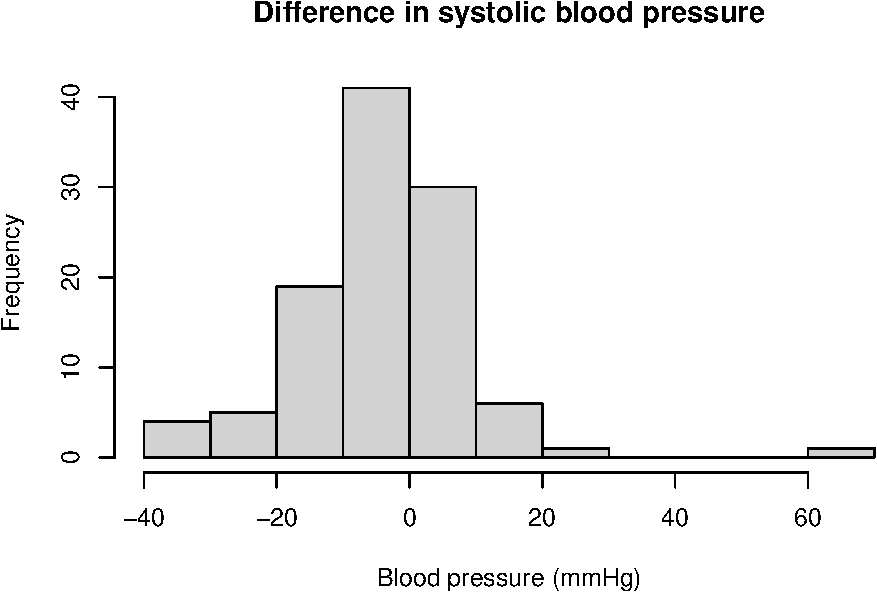
\includegraphics{phcm9795-R-notes_files/figure-latex/unnamed-chunk-93-1.pdf}

To add a fitted line, we can use the \texttt{abline()} function which adds a straight line to the plot. The equation of this straight line will be determined from the estimated regression line, which we specify with \texttt{lm(y\ \textasciitilde{}\ x)}. Putting this all together:

\begin{Shaded}
\begin{Highlighting}[]
\FunctionTok{plot}\NormalTok{(}\AttributeTok{x=}\NormalTok{lung}\SpecialCharTok{$}\NormalTok{Height, }\AttributeTok{y=}\NormalTok{lung}\SpecialCharTok{$}\NormalTok{FVC, }\AttributeTok{xlab=}\StringTok{"Height (cm)"}\NormalTok{, }\AttributeTok{ylab=}\StringTok{"Forced vital capacity (L)"}\NormalTok{)}
\FunctionTok{abline}\NormalTok{(}\FunctionTok{lm}\NormalTok{(lung}\SpecialCharTok{$}\NormalTok{FVC }\SpecialCharTok{\textasciitilde{}}\NormalTok{ lung}\SpecialCharTok{$}\NormalTok{Height))}
\end{Highlighting}
\end{Shaded}

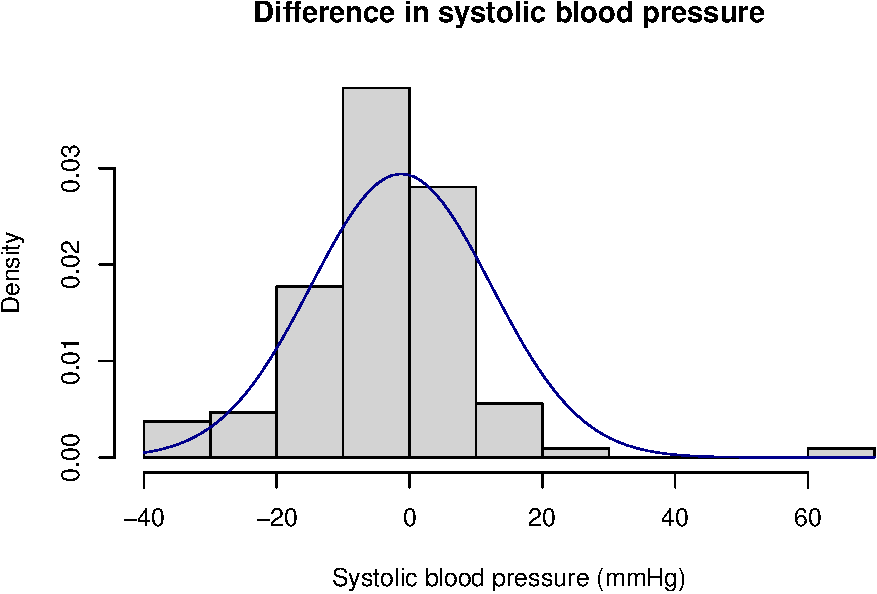
\includegraphics{phcm9795-R-notes_files/figure-latex/unnamed-chunk-94-1.pdf}

To create a scatter plot using \texttt{ggplot2}, we define the x and y aesthetics as the \texttt{Height} and \texttt{FVC}. We then specify that we want to plot points, by specifying the point geometry using \texttt{geom\_point}. We can add labels in the usual way. Putting it all together:

\begin{Shaded}
\begin{Highlighting}[]
\FunctionTok{ggplot}\NormalTok{(}\AttributeTok{data=}\NormalTok{lung, }\FunctionTok{aes}\NormalTok{(}\AttributeTok{x=}\NormalTok{Height, }\AttributeTok{y=}\NormalTok{FVC)) }\SpecialCharTok{+} 
  \FunctionTok{geom\_point}\NormalTok{() }\SpecialCharTok{+}
  \FunctionTok{labs}\NormalTok{(}\AttributeTok{x=}\StringTok{"Height (cm)"}\NormalTok{, }\AttributeTok{y=}\StringTok{"Forced vital capacity (L)"}\NormalTok{)}
\end{Highlighting}
\end{Shaded}

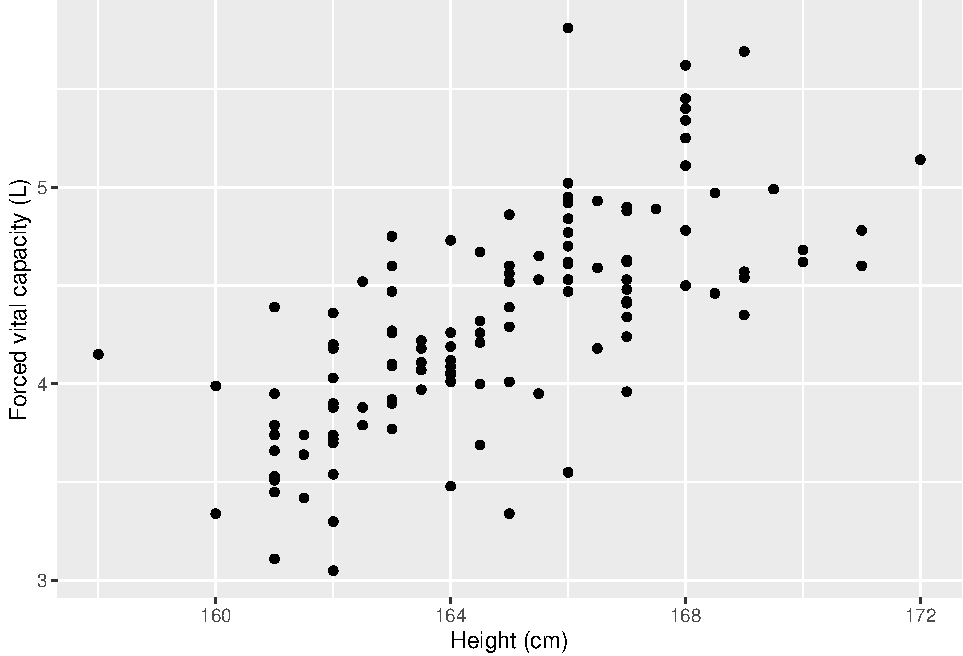
\includegraphics{phcm9795-R-notes_files/figure-latex/unnamed-chunk-95-1.pdf}

We can add an estimated regression line by adding a \texttt{geom\_smooth}, specifying that the line should be based on a linear model (\texttt{lm}), and no error shading should be included (\texttt{se=FALSE}):

\begin{Shaded}
\begin{Highlighting}[]
\FunctionTok{ggplot}\NormalTok{(}\AttributeTok{data=}\NormalTok{lung, }\FunctionTok{aes}\NormalTok{(}\AttributeTok{x=}\NormalTok{Height, }\AttributeTok{y=}\NormalTok{FVC)) }\SpecialCharTok{+} 
  \FunctionTok{geom\_point}\NormalTok{() }\SpecialCharTok{+}
  \FunctionTok{geom\_smooth}\NormalTok{(}\AttributeTok{method=}\NormalTok{lm, }\AttributeTok{se=}\ConstantTok{FALSE}\NormalTok{) }\SpecialCharTok{+}
  \FunctionTok{labs}\NormalTok{(}\AttributeTok{x=}\StringTok{"Height (cm)"}\NormalTok{, }\AttributeTok{y=}\StringTok{"Forced vital capacity (L)"}\NormalTok{)}
\end{Highlighting}
\end{Shaded}

\begin{verbatim}
## `geom_smooth()` using formula 'y ~ x'
\end{verbatim}

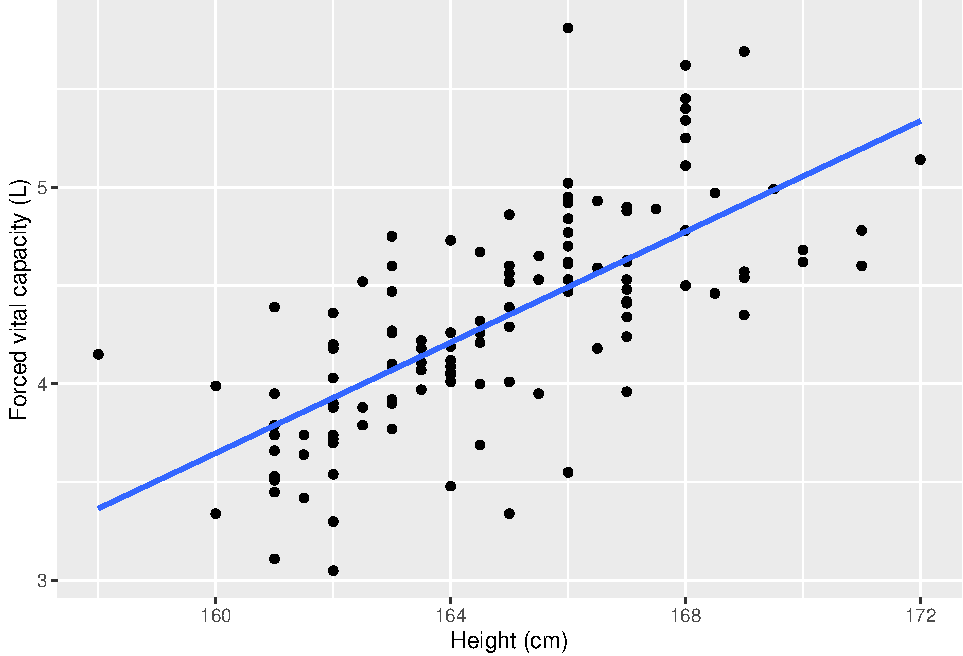
\includegraphics{phcm9795-R-notes_files/figure-latex/unnamed-chunk-96-1.pdf}

\hypertarget{calculating-a-correlation-coefficient}{%
\section{Calculating a correlation coefficient}\label{calculating-a-correlation-coefficient}}

We can use the \texttt{cor.test} function to calculate a Pearson's correlation coefficient:

\begin{Shaded}
\begin{Highlighting}[]
\FunctionTok{cor.test}\NormalTok{(lung}\SpecialCharTok{$}\NormalTok{Height, lung}\SpecialCharTok{$}\NormalTok{FVC)}
\end{Highlighting}
\end{Shaded}

\begin{verbatim}
## 
##  Pearson's product-moment correlation
## 
## data:  lung$Height and lung$FVC
## t = 10.577, df = 118, p-value < 2.2e-16
## alternative hypothesis: true correlation is not equal to 0
## 95 percent confidence interval:
##  0.5924715 0.7794090
## sample estimates:
##      cor 
## 0.697628
\end{verbatim}

\hypertarget{fitting-a-simple-linear-regression-model}{%
\section{Fitting a simple linear regression model}\label{fitting-a-simple-linear-regression-model}}

We can use the \texttt{lm} function to fit a simple linear regression model, specifying the model as \texttt{y\ \textasciitilde{}\ x}. Using \texttt{Example\_8.1.dta}, we can quantify the relationship between FVC and height.

\begin{Shaded}
\begin{Highlighting}[]
\FunctionTok{lm}\NormalTok{(FVC }\SpecialCharTok{\textasciitilde{}}\NormalTok{ Height, }\AttributeTok{data=}\NormalTok{lung)}
\end{Highlighting}
\end{Shaded}

\begin{verbatim}
## 
## Call:
## lm(formula = FVC ~ Height, data = lung)
## 
## Coefficients:
## (Intercept)       Height  
##    -18.8735       0.1408
\end{verbatim}

The default output from the \texttt{lm} function is rather sparse. We can obtain much more useful information by defining the model as an object, then using the \texttt{summary()} function:

\begin{Shaded}
\begin{Highlighting}[]
\NormalTok{model1 }\OtherTok{\textless{}{-}} \FunctionTok{lm}\NormalTok{(FVC }\SpecialCharTok{\textasciitilde{}}\NormalTok{ Height, }\AttributeTok{data=}\NormalTok{lung)}
\FunctionTok{summary}\NormalTok{(model1)}
\end{Highlighting}
\end{Shaded}

\begin{verbatim}
## 
## Call:
## lm(formula = FVC ~ Height, data = lung)
## 
## Residuals:
##      Min       1Q   Median       3Q      Max 
## -1.01139 -0.23643 -0.02082  0.24918  1.31786 
## 
## Coefficients:
##              Estimate Std. Error t value Pr(>|t|)    
## (Intercept) -18.87347    2.19365  -8.604 3.89e-14 ***
## Height        0.14076    0.01331  10.577  < 2e-16 ***
## ---
## Signif. codes:  0 '***' 0.001 '**' 0.01 '*' 0.05 '.' 0.1 ' ' 1
## 
## Residual standard error: 0.3965 on 118 degrees of freedom
## Multiple R-squared:  0.4867, Adjusted R-squared:  0.4823 
## F-statistic: 111.9 on 1 and 118 DF,  p-value: < 2.2e-16
\end{verbatim}

Finally, we can obtain 95\% confidence intervals for the regression coefficients using the \texttt{confint} function:

\begin{Shaded}
\begin{Highlighting}[]
\FunctionTok{confint}\NormalTok{(model1)}
\end{Highlighting}
\end{Shaded}

\begin{verbatim}
##                   2.5 %      97.5 %
## (Intercept) -23.2174967 -14.5294444
## Height        0.1144042   0.1671092
\end{verbatim}

\hypertarget{plotting-residuals-from-a-simple-linear-regression}{%
\section{Plotting residuals from a simple linear regression}\label{plotting-residuals-from-a-simple-linear-regression}}

We can use the \texttt{resid} function to obtain the residuals from a saved model. These residuals can then be plotted using a histogram in the usual way:

\begin{Shaded}
\begin{Highlighting}[]
\NormalTok{residuals }\OtherTok{\textless{}{-}} \FunctionTok{resid}\NormalTok{(model1)}
\FunctionTok{hist}\NormalTok{(residuals)}
\end{Highlighting}
\end{Shaded}

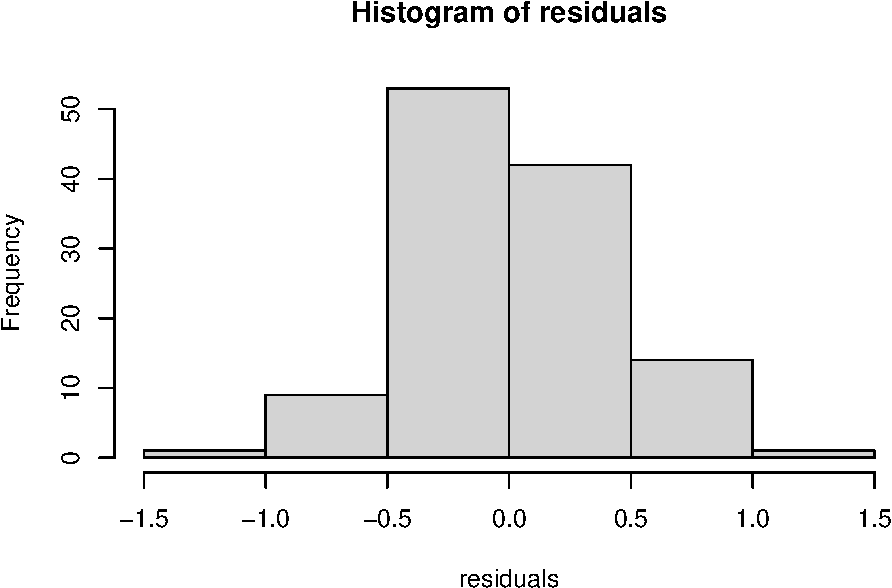
\includegraphics{phcm9795-R-notes_files/figure-latex/unnamed-chunk-101-1.pdf}

A Normal curve can be overlaid if we plot the residuals using a probability scale.

\begin{Shaded}
\begin{Highlighting}[]
\FunctionTok{hist}\NormalTok{(residuals, }\AttributeTok{probability =} \ConstantTok{TRUE}\NormalTok{, }\AttributeTok{ylim=}\FunctionTok{c}\NormalTok{(}\DecValTok{0}\NormalTok{,}\DecValTok{1}\NormalTok{))}
\FunctionTok{curve}\NormalTok{(}\FunctionTok{dnorm}\NormalTok{(x, }\AttributeTok{mean=}\FunctionTok{mean}\NormalTok{(residuals), }\AttributeTok{sd=}\FunctionTok{sd}\NormalTok{(residuals)), }
      \AttributeTok{col=}\StringTok{"darkblue"}\NormalTok{, }\AttributeTok{lwd=}\DecValTok{2}\NormalTok{, }\AttributeTok{add=}\ConstantTok{TRUE}\NormalTok{)}
\end{Highlighting}
\end{Shaded}

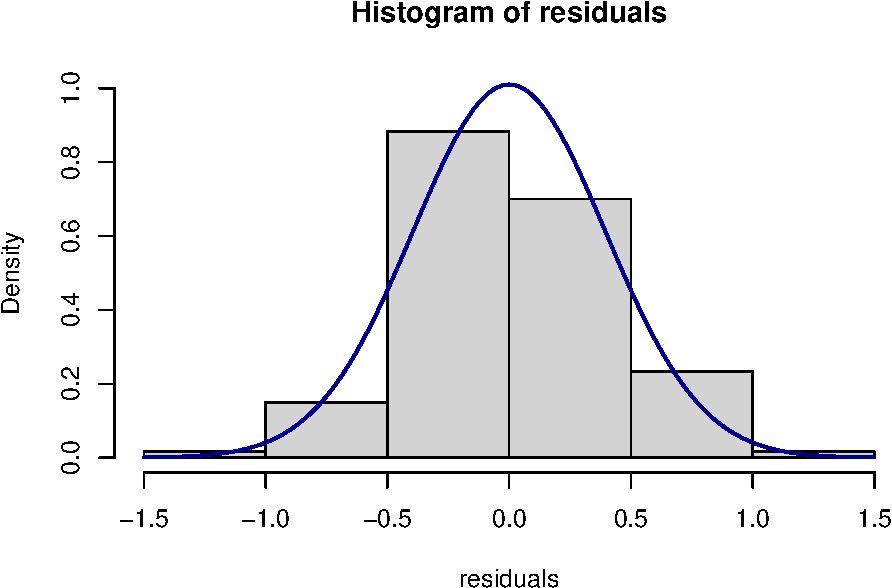
\includegraphics{phcm9795-R-notes_files/figure-latex/unnamed-chunk-102-1.pdf}

Alternatively, a \texttt{ggplot2} approach can be used, after converting the single vector of residuals into a dataframe:

\begin{Shaded}
\begin{Highlighting}[]
\NormalTok{resid }\OtherTok{\textless{}{-}} \FunctionTok{as.data.frame}\NormalTok{(residuals)}

\FunctionTok{ggplot}\NormalTok{(resid, }\FunctionTok{aes}\NormalTok{(}\AttributeTok{x=}\NormalTok{residuals)) }\SpecialCharTok{+} 
  \FunctionTok{geom\_histogram}\NormalTok{(}\AttributeTok{binwidth =} \FloatTok{0.5}\NormalTok{, }\AttributeTok{boundary=}\SpecialCharTok{{-}}\FloatTok{1.5}\NormalTok{, }\AttributeTok{colour=}\StringTok{"black"}\NormalTok{, }\AttributeTok{fill=}\StringTok{"white"}\NormalTok{)}
\end{Highlighting}
\end{Shaded}

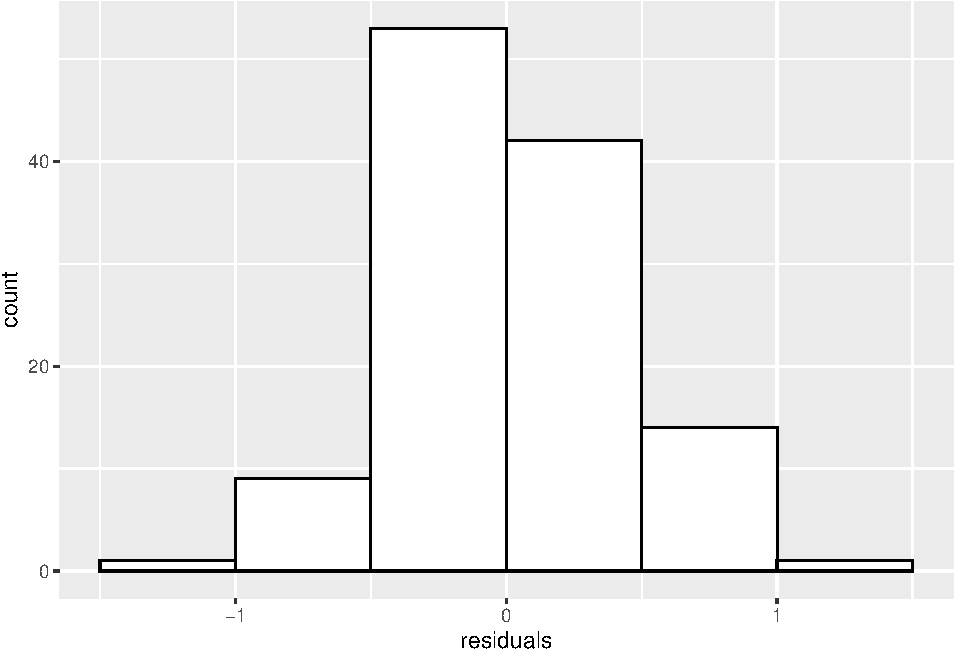
\includegraphics{phcm9795-R-notes_files/figure-latex/unnamed-chunk-103-1.pdf}

\begin{Shaded}
\begin{Highlighting}[]
\FunctionTok{ggplot}\NormalTok{(resid, }\FunctionTok{aes}\NormalTok{(}\AttributeTok{x=}\NormalTok{residuals)) }\SpecialCharTok{+} 
  \FunctionTok{geom\_histogram}\NormalTok{(}\FunctionTok{aes}\NormalTok{(}\AttributeTok{y =}\NormalTok{ ..density..), }\AttributeTok{binwidth =} \FloatTok{0.5}\NormalTok{, }\AttributeTok{boundary=}\SpecialCharTok{{-}}\FloatTok{1.5}\NormalTok{, }\AttributeTok{colour=}\StringTok{"black"}\NormalTok{, }\AttributeTok{fill=}\StringTok{"white"}\NormalTok{) }\SpecialCharTok{+}
  \FunctionTok{stat\_function}\NormalTok{(}\AttributeTok{fun =}\NormalTok{ dnorm, }\AttributeTok{args =} \FunctionTok{list}\NormalTok{(}\AttributeTok{mean =} \FunctionTok{mean}\NormalTok{(resid}\SpecialCharTok{$}\NormalTok{residuals), }\AttributeTok{sd =} \FunctionTok{sd}\NormalTok{(resid}\SpecialCharTok{$}\NormalTok{residuals)))}
\end{Highlighting}
\end{Shaded}

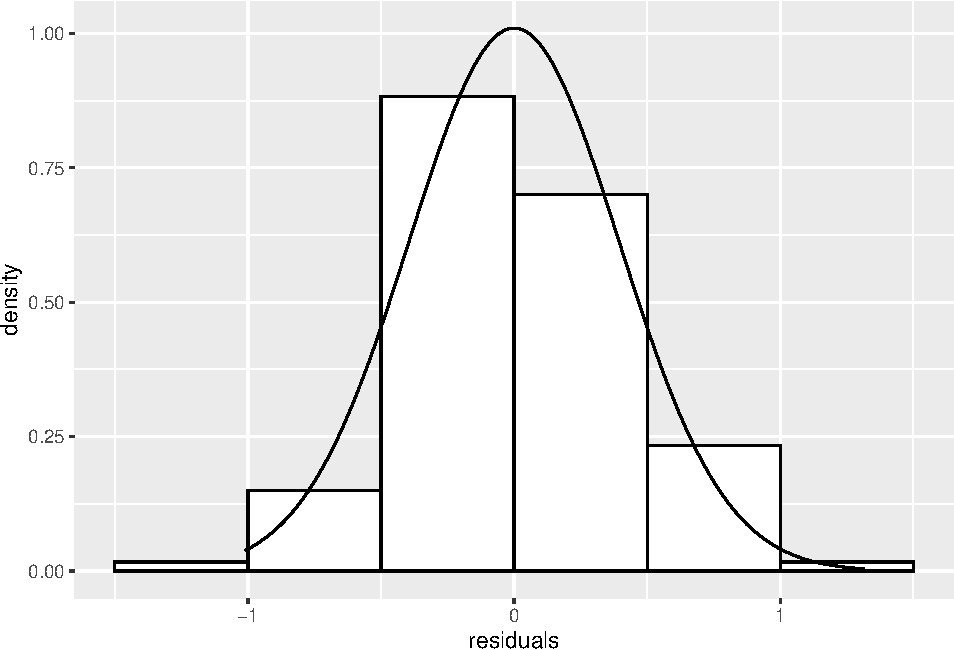
\includegraphics{phcm9795-R-notes_files/figure-latex/unnamed-chunk-103-2.pdf}

\hypertarget{analysing-non-normal-data}{%
\chapter{Analysing non-normal data}\label{analysing-non-normal-data}}

\hypertarget{transforming-non-normally-distributed-variables}{%
\section{Transforming non-normally distributed variables}\label{transforming-non-normally-distributed-variables}}

One option for dealing with a non-normally distributed varaible is to transform it into its square, square root or logarithmic value. The new transformed variable may be normally distributed and therefore a parametric test can be used. First we check the distribution of the variable for normality, e.g.~by plotting a histogram.

You can calculate a new, transformed, variable using variable transformation commands. For example, to create a new column of data based on the log of length of stay using Base R:

\begin{Shaded}
\begin{Highlighting}[]
\FunctionTok{library}\NormalTok{(haven)      }\CommentTok{\# For importing data}
\FunctionTok{library}\NormalTok{(labelled)}

\NormalTok{hospital }\OtherTok{\textless{}{-}} \FunctionTok{unlabelled}\NormalTok{(}\FunctionTok{read\_dta}\NormalTok{(}\StringTok{"/Users/td/Documents/GithubRepos/phcm9795/data/examples/Example\_9.1.dta"}\NormalTok{))}

\NormalTok{hospital}\SpecialCharTok{$}\NormalTok{ln\_los }\OtherTok{\textless{}{-}} \FunctionTok{log}\NormalTok{(hospital}\SpecialCharTok{$}\NormalTok{los}\SpecialCharTok{+}\DecValTok{1}\NormalTok{)}
\FunctionTok{summary}\NormalTok{(hospital)}
\end{Highlighting}
\end{Shaded}

\begin{verbatim}
##        id            gender               los         infect         surgery  
##  Min.   : 10.00   Length:132         Min.   :  0.00   No :106   Abdominal:48  
##  1st Qu.: 42.75   Class :character   1st Qu.: 20.75   Yes: 26   Cardiac  :53  
##  Median : 75.50   Mode  :character   Median : 27.00             Other    :31  
##  Mean   : 75.50                      Mean   : 38.05                           
##  3rd Qu.:108.25                      3rd Qu.: 42.00                           
##  Max.   :141.00                      Max.   :244.00                           
##      ln_los     
##  Min.   :0.000  
##  1st Qu.:3.079  
##  Median :3.332  
##  Mean   :3.407  
##  3rd Qu.:3.761  
##  Max.   :5.501
\end{verbatim}

A tidyverse version uses the \texttt{mutate} command to create a new variable:

\begin{Shaded}
\begin{Highlighting}[]
\FunctionTok{library}\NormalTok{(tidyverse)}

\NormalTok{hospital }\OtherTok{\textless{}{-}} \FunctionTok{read\_dta}\NormalTok{(}\StringTok{"/Users/td/Documents/GithubRepos/phcm9795/data/examples/Example\_9.1.dta"}\NormalTok{) }\SpecialCharTok{\%\textgreater{}\%} 
  \FunctionTok{unlabelled}\NormalTok{()}

\NormalTok{hospital }\OtherTok{\textless{}{-}}\NormalTok{ hospital }\SpecialCharTok{\%\textgreater{}\%} 
  \FunctionTok{mutate}\NormalTok{(}\AttributeTok{ln\_los =} \FunctionTok{log}\NormalTok{(los}\SpecialCharTok{+}\DecValTok{1}\NormalTok{))}

\FunctionTok{summary}\NormalTok{(hospital)}
\end{Highlighting}
\end{Shaded}

\begin{verbatim}
##        id            gender               los         infect         surgery  
##  Min.   : 10.00   Length:132         Min.   :  0.00   No :106   Abdominal:48  
##  1st Qu.: 42.75   Class :character   1st Qu.: 20.75   Yes: 26   Cardiac  :53  
##  Median : 75.50   Mode  :character   Median : 27.00             Other    :31  
##  Mean   : 75.50                      Mean   : 38.05                           
##  3rd Qu.:108.25                      3rd Qu.: 42.00                           
##  Max.   :141.00                      Max.   :244.00                           
##      ln_los     
##  Min.   :0.000  
##  1st Qu.:3.079  
##  Median :3.332  
##  Mean   :3.407  
##  3rd Qu.:3.761  
##  Max.   :5.501
\end{verbatim}

You can now check whether this logged variable is normally distributed as described in Module 2, for example by plotting a histogram as shown in Figure 9.2.

To obtain the back-transformed mean shown in Output 9.1, we can use the \texttt{exp} command:

\begin{Shaded}
\begin{Highlighting}[]
\FunctionTok{exp}\NormalTok{(}\FloatTok{3.407232}\NormalTok{)}
\end{Highlighting}
\end{Shaded}

\begin{verbatim}
## [1] 30.18159
\end{verbatim}

If your transformed variable is approximately normally distributed, you can apply parametric tests such as the t-test. In the Worked Example 9.1 dataset, the variable \texttt{infect} (presence of nosocomial infection) is a binary categorical variable. To test the hypothesis that patients with nosocomial infection have a different length of stay to patients without infection, you can conduct a t-test on the \texttt{ln\_los} variable. You will need to back transform your mean values, as shown in Worked Example 9.1 in the course notes when reporting your results.

\hypertarget{wilcoxon-ranked-sum-test}{%
\section{Wilcoxon ranked-sum test}\label{wilcoxon-ranked-sum-test}}

We use the \texttt{wilcox.test} function to perform the Wilcoxon ranked-sum test:

\begin{verbatim}
wilcox.test(continuous_variable ~ group_variable, data=df, correct=FALSE)
\end{verbatim}

The Wilcoxon ranked-sum test will be demonstrated using the length of stay data in \texttt{Example\_9.1.dta}. Here, out continuous variable is \texttt{los} and the grouping variable is \texttt{infect}.

\begin{Shaded}
\begin{Highlighting}[]
\FunctionTok{wilcox.test}\NormalTok{(los }\SpecialCharTok{\textasciitilde{}}\NormalTok{ infect, }\AttributeTok{data=}\NormalTok{hospital, }\AttributeTok{correct=}\ConstantTok{FALSE}\NormalTok{)}
\end{Highlighting}
\end{Shaded}

\begin{verbatim}
## 
##  Wilcoxon rank sum test
## 
## data:  los by infect
## W = 949, p-value = 0.01402
## alternative hypothesis: true location shift is not equal to 0
\end{verbatim}

\hypertarget{wilcoxon-matched-pairs-signed-rank-test}{%
\section{Wilcoxon matched-pairs signed-rank test}\label{wilcoxon-matched-pairs-signed-rank-test}}

The \texttt{wilcox.test} function can also be used to conduct the Wilcoxon matched-pairs signed-rank test. The specification of the variables is a little different, in that each variable is specified as \texttt{dataframe\$variable}:

\begin{verbatim}
wilcox.test(df$continuous_variable_1, df$continuous_variable_1, paired=TRUE)
\end{verbatim}

We will demonstrate using the dataset on the arthritis drug cross-over trial (\texttt{Example\_9.2.dta}). Like the paired t-test the paired data need to be in separate columns.

\begin{Shaded}
\begin{Highlighting}[]
\NormalTok{arthritis }\OtherTok{\textless{}{-}} \FunctionTok{read\_dta}\NormalTok{(}\StringTok{"/Users/td/Documents/GithubRepos/phcm9795/data/examples/Example\_9.2.dta"}\NormalTok{) }\SpecialCharTok{\%\textgreater{}\%} 
  \FunctionTok{unlabelled}\NormalTok{()}

\NormalTok{arthritis}\SpecialCharTok{$}\NormalTok{difference }\OtherTok{=}\NormalTok{ arthritis}\SpecialCharTok{$}\NormalTok{drug\_1 }\SpecialCharTok{{-}}\NormalTok{ arthritis}\SpecialCharTok{$}\NormalTok{drug\_2}

\FunctionTok{hist}\NormalTok{(arthritis}\SpecialCharTok{$}\NormalTok{difference, }\AttributeTok{xlab=}\StringTok{"Difference"}\NormalTok{, }\AttributeTok{main=}\StringTok{"Histogram of differences in pain scores"}\NormalTok{)}
\end{Highlighting}
\end{Shaded}

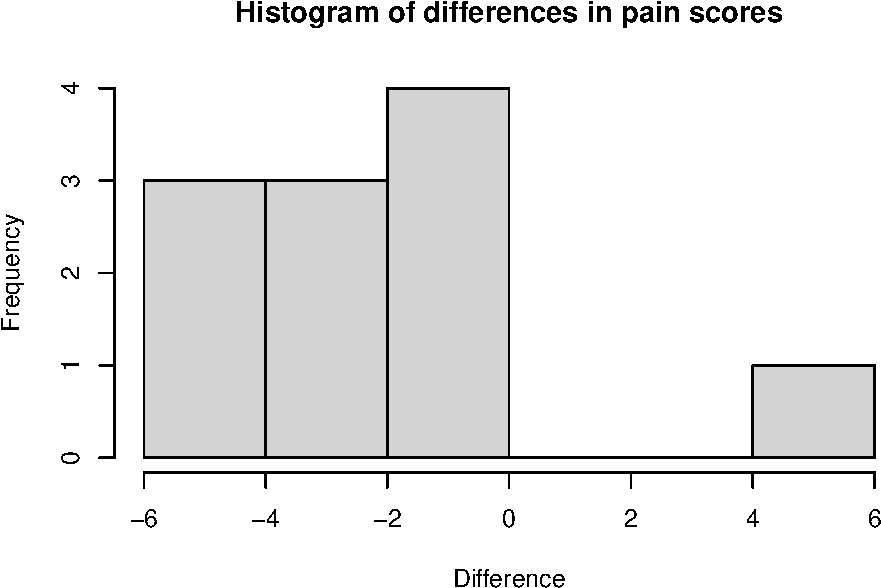
\includegraphics{phcm9795-R-notes_files/figure-latex/unnamed-chunk-108-1.pdf}

\begin{Shaded}
\begin{Highlighting}[]
\FunctionTok{wilcox.test}\NormalTok{(arthritis}\SpecialCharTok{$}\NormalTok{drug\_1, arthritis}\SpecialCharTok{$}\NormalTok{drug\_2, }\AttributeTok{paired=}\ConstantTok{TRUE}\NormalTok{)}
\end{Highlighting}
\end{Shaded}

\begin{verbatim}
## Warning in wilcox.test.default(arthritis$drug_1, arthritis$drug_2, paired =
## TRUE): cannot compute exact p-value with ties
\end{verbatim}

\begin{verbatim}
## 
##  Wilcoxon signed rank test with continuity correction
## 
## data:  arthritis$drug_1 and arthritis$drug_2
## V = 10.5, p-value = 0.04898
## alternative hypothesis: true location shift is not equal to 0
\end{verbatim}

\hypertarget{estimating-rank-correlation-coefficients}{%
\section{Estimating rank correlation coefficients}\label{estimating-rank-correlation-coefficients}}

The analyses for Spearman's and Kendall's rank correlation are conducted in similar ways:

\begin{Shaded}
\begin{Highlighting}[]
\NormalTok{lung }\OtherTok{\textless{}{-}} \FunctionTok{read\_dta}\NormalTok{(}\StringTok{"/Users/td/Documents/GithubRepos/phcm9795/data/examples/Example\_8.1.dta"}\NormalTok{)}

\FunctionTok{cor.test}\NormalTok{(lung}\SpecialCharTok{$}\NormalTok{Height, lung}\SpecialCharTok{$}\NormalTok{FVC, }\AttributeTok{method=}\StringTok{"spearman"}\NormalTok{)}
\end{Highlighting}
\end{Shaded}

\begin{verbatim}
## Warning in cor.test.default(lung$Height, lung$FVC, method = "spearman"): Cannot
## compute exact p-value with ties
\end{verbatim}

\begin{verbatim}
## 
##  Spearman's rank correlation rho
## 
## data:  lung$Height and lung$FVC
## S = 72699, p-value < 2.2e-16
## alternative hypothesis: true rho is not equal to 0
## sample estimates:
##       rho 
## 0.7475566
\end{verbatim}

\begin{Shaded}
\begin{Highlighting}[]
\FunctionTok{cor.test}\NormalTok{(lung}\SpecialCharTok{$}\NormalTok{Height, lung}\SpecialCharTok{$}\NormalTok{FVC, }\AttributeTok{method=}\StringTok{"kendall"}\NormalTok{)}
\end{Highlighting}
\end{Shaded}

\begin{verbatim}
## 
##  Kendall's rank correlation tau
## 
## data:  lung$Height and lung$FVC
## z = 8.8244, p-value < 2.2e-16
## alternative hypothesis: true tau is not equal to 0
## sample estimates:
##       tau 
## 0.5609431
\end{verbatim}

\hypertarget{sample-size}{%
\chapter{Sample size}\label{sample-size}}

Many power and sample size procedures are available in the \texttt{epiR} package.

\begin{Shaded}
\begin{Highlighting}[]
\CommentTok{\# If not yet installed, submit the following:}
\CommentTok{\# install.packages("epiR")}
\FunctionTok{library}\NormalTok{(epiR)}
\end{Highlighting}
\end{Shaded}

\hypertarget{sample-size-calculation-for-two-independent-samples-t-test}{%
\section{Sample size calculation for two independent samples t-test}\label{sample-size-calculation-for-two-independent-samples-t-test}}

To do the problem discussed in Worked Example 10.2, we use the \texttt{epi.sscompc} function: \textbf{Sample size, power and minimum detectable difference when comparing continuous outcomes}.

\begin{verbatim}
epi.sscompc(treat, control, n, sigma, power, 
   r = 1, design = 1, sided.test = 2, nfractional = FALSE, conf.level = 0.95)
\end{verbatim}

The first line contains parameters that we can specify, with one parameter that is to be calculated. That is, we define values for four of the five parameters, and the remaining parameter is calculated. For example, we can define the mean in the treated group, the mean in the control group, the assumed standard deviation and the desired power, and the function will calculate the required sample size. We specify the unknown value as being equal to R's missing value, \texttt{NA}.

For example, to calculate the required sample size in Worked Example 10.2, we specify:

\begin{itemize}
\tightlist
\item
  the assumed mean in the experimental, or treatment, group: 90mmHg
\item
  the assumed mean in the control group: 95mmHg
\item
  the standard deviation of blood pressure: 5mmHg
\item
  the required power, 0.9 (representing 90\%)
\end{itemize}

The values on the second line of the function are defined by default, and we can leave these as default.

Putting this all together, and specifying the sample size as unknown:

\begin{Shaded}
\begin{Highlighting}[]
\FunctionTok{epi.sscompc}\NormalTok{(}\AttributeTok{treat=}\DecValTok{90}\NormalTok{, }\AttributeTok{control=}\DecValTok{95}\NormalTok{, }\AttributeTok{n=}\ConstantTok{NA}\NormalTok{, }\AttributeTok{sigma=}\DecValTok{5}\NormalTok{, }\AttributeTok{power=}\FloatTok{0.9}\NormalTok{) }
\end{Highlighting}
\end{Shaded}

\begin{verbatim}
## $n.total
## [1] 44
## 
## $n.treat
## [1] 22
## 
## $n.control
## [1] 22
## 
## $power
## [1] 0.9
## 
## $delta
## [1] 5
\end{verbatim}

The results indicate that we need 22 participants in each group, or 44 in total.

We can define whether we want unequal numbers in each group by specifying \texttt{r}: the number in the treatment group divided by the number in the control group.

\hypertarget{sample-size-calculation-for-difference-between-two-independent-proportions}{%
\section{Sample size calculation for difference between two independent proportions}\label{sample-size-calculation-for-difference-between-two-independent-proportions}}

To do the problem discussed in Worked Example 10.3, we use the \texttt{epi.sscohortc} function: \textbf{Sample size, power or minimum detectable incidence risk ratio for a cohort study using individual count data}.

\begin{verbatim}
epi.sscohortc(irexp1, irexp0, pexp = NA, n = NA, power = 0.80, 
   r = 1, N, design = 1, sided.test = 2, finite.correction = FALSE, 
   nfractional = FALSE, conf.level = 0.95)
\end{verbatim}

We can enter:

\begin{itemize}
\tightlist
\item
  irexp1: the assumed risk of the outcome in the exposed group: here 0.35
\item
  irexp0: the assumed risk of the outcome in the unexposed group: here 0.2
\item
  n: the total sample size, to be determined
\item
  power: the required power: here 0.8 (representing 80\%)
\end{itemize}

\begin{Shaded}
\begin{Highlighting}[]
\FunctionTok{epi.sscohortc}\NormalTok{(}\AttributeTok{irexp1=}\FloatTok{0.35}\NormalTok{, }\AttributeTok{irexp0=}\FloatTok{0.2}\NormalTok{, }\AttributeTok{n=}\ConstantTok{NA}\NormalTok{, }\AttributeTok{power=}\FloatTok{0.8}\NormalTok{) }
\end{Highlighting}
\end{Shaded}

\begin{verbatim}
## $n.total
## [1] 276
## 
## $n.exp1
## [1] 138
## 
## $n.exp0
## [1] 138
## 
## $power
## [1] 0.8
## 
## $irr
## [1] 1.75
## 
## $or
## [1] 2.153846
\end{verbatim}

Note: It doesn't matter if you swap the proportions for the \textbf{exposed} and \textbf{unexposed} groups, i.e.~the command \texttt{epi.sscohortc(irexp1=0.2,\ irexp0=0.35,\ n=NA,\ power=0.8)} gives the same results.

\hypertarget{sample-size-calculation-with-a-relative-risk}{%
\section{Sample size calculation with a relative risk}\label{sample-size-calculation-with-a-relative-risk}}

The \texttt{epiR} package does not have a function to estimate sample size and power directly for a relative risk, but we can use the \texttt{epi.sscohortc} function.

\hypertarget{sample-size-calculation-with-an-odds-ratio}{%
\section{Sample size calculation with an odds ratio}\label{sample-size-calculation-with-an-odds-ratio}}

We can use the \texttt{epi.sscc} function to calculate a sample size based on an odds ratio in a case-control study:

\begin{verbatim}
epi.sscc(OR, p1 = NA, p0, n, power, r = 1, 
   phi.coef = 0, design = 1, sided.test = 2, nfractional = FALSE, 
   conf.level = 0.95, method = "unmatched", fleiss = FALSE)
\end{verbatim}

Using information from Worked Example 10.4, we specify:

\begin{itemize}
\tightlist
\item
  OR: the odds ratio to be detected, here 1.5
\item
  p0: the proportion of the outcome in the controls, here 0.5
\item
  n: the sample size, here to be calculated
\item
  power: the required study power, here 0.9
\end{itemize}

\begin{Shaded}
\begin{Highlighting}[]
\FunctionTok{epi.sscc}\NormalTok{(}\AttributeTok{OR=}\FloatTok{1.5}\NormalTok{, }\AttributeTok{p0=}\FloatTok{0.5}\NormalTok{, }\AttributeTok{n=}\ConstantTok{NA}\NormalTok{, }\AttributeTok{power=}\FloatTok{0.9}\NormalTok{)}
\end{Highlighting}
\end{Shaded}

\begin{verbatim}
## $n.total
## [1] 1038
## 
## $n.case
## [1] 519
## 
## $n.control
## [1] 519
## 
## $power
## [1] 0.9
## 
## $OR
## [1] 1.5
\end{verbatim}

Now we calculate the sample size for Worked Example 10.5:

\begin{Shaded}
\begin{Highlighting}[]
\FunctionTok{epi.sscc}\NormalTok{(}\AttributeTok{OR=}\DecValTok{2}\NormalTok{, }\AttributeTok{p0=}\FloatTok{0.3}\NormalTok{, }\AttributeTok{n=}\ConstantTok{NA}\NormalTok{, }\AttributeTok{power=}\FloatTok{0.9}\NormalTok{)}
\end{Highlighting}
\end{Shaded}

\begin{verbatim}
## $n.total
## [1] 376
## 
## $n.case
## [1] 188
## 
## $n.control
## [1] 188
## 
## $power
## [1] 0.9
## 
## $OR
## [1] 2
\end{verbatim}

Here we see that we require a total of 376 participants to detect an odds ratio of 2.0 with 90\% power;

\begin{Shaded}
\begin{Highlighting}[]
\FunctionTok{epi.sscc}\NormalTok{(}\AttributeTok{OR=}\DecValTok{2}\NormalTok{, }\AttributeTok{p0=}\FloatTok{0.3}\NormalTok{, }\AttributeTok{n=}\ConstantTok{NA}\NormalTok{, }\AttributeTok{power=}\FloatTok{0.8}\NormalTok{)}
\end{Highlighting}
\end{Shaded}

\begin{verbatim}
## $n.total
## [1] 282
## 
## $n.case
## [1] 141
## 
## $n.control
## [1] 141
## 
## $power
## [1] 0.8
## 
## $OR
## [1] 2
\end{verbatim}

or a total of 282 participants to detect an odds ratio of 2.0 with 80\% power.

  \bibliography{PHCM9795.bib}

\end{document}
